% ============================================================================
% 论文初稿: Homogenization bias and applicability limits of orientation-resolved
% ductile damage descriptors in AM alloys under Taylor crystal plasticity
% Target Journal: International Journal of Plasticity
% ============================================================================

% ============================================================================
% IJDM submission build using the official SAGE sagej.cls template.
% Layout: A4 two-column + numbered references (no natbib); body and bibliography
% are byte-identical to manuscript_main.tex. The geometry package is not
% installed on this offline machine, so the sagej "Afour" option (which would
% load it) is not used; the A4 two-column text block is set natively below,
% mirroring the manual \textwidth/\oddsidemargin approach of manuscript_main.tex.
% ============================================================================
\documentclass[twocolumn]{sagej}
\usepackage[utf8]{inputenc}
\usepackage{array}
\usepackage{multirow}
\usepackage{xcolor}
\usepackage{float}
\usepackage{siunitx}
\usepackage{tikz}
\usetikzlibrary{arrows.meta,positioning}
% Let justified text stretch a little to avoid overfull lines in narrow columns.
\setlength{\emergencystretch}{2.5em}
% sagej typesets sections unnumbered by default (secnumdepth=-2); the manuscript
% cross-references numbered sections via Section~\ref{...}, so restore numbering.
\setcounter{secnumdepth}{2}
\usepackage[colorlinks=true,linkcolor=blue,citecolor=blue,urlcolor=blue]{hyperref}

% ---- A4 two-column text block (native, geometry not installed) ----
\usepackage{ftnright}
\setlength{\paperwidth}{210mm}\setlength{\paperheight}{297mm}
\pdfpagewidth=\paperwidth\pdfpageheight=\paperheight
\setlength{\textwidth}{174mm}
\setlength{\oddsidemargin}{-7.4mm}\setlength{\evensidemargin}{-7.4mm}
\setlength{\topmargin}{-14mm}
\setlength{\headheight}{14pt}\setlength{\headsep}{21pt}
\setlength{\textheight}{248mm}
\setlength{\columnsep}{12pt}\setlength{\footskip}{25pt}
% ---- Float packing: allow multiple full-width (figure*/table*) floats at the
% top of a page and reduce large white gaps left by the full-width figures. ----
\setcounter{topnumber}{3}
\setcounter{dbltopnumber}{3}
\setcounter{totalnumber}{6}
\renewcommand{\topfraction}{0.92}
\renewcommand{\dbltopfraction}{0.92}
\renewcommand{\textfraction}{0.06}
\renewcommand{\floatpagefraction}{0.95}
\renewcommand{\dblfloatpagefraction}{0.95}

% ---- sagej front matter ----
\runninghead{Wang et al.}
\def\volumeyear{2026}
\def\journalname{International Journal of Damage Mechanics}
\title{A leakage-free validation framework for quantifying Taylor homogenization bias and mapping the applicability domain---when orientation-resolved ductile damage descriptors help and when they do not---in additively manufactured metals}
\author{Han Wang\affilnum{1,*}, Lu Zhang\affilnum{1}, Anna Stepashkina\affilnum{1}, and Qi Hu\affilnum{2}}
\affiliation{\affilnum{1}Zhejiang Lab, 2880 Wenyi West Rd, Hangzhou 311121, China\\ \affilnum{2}Department of Plasticity Technology, School of Materials Science and Engineering, Shanghai Jiao Tong University, Shanghai 200030, PR China}
\corrauth{Han Wang, Zhejiang Lab, 2880 Wenyi West Rd, Hangzhou 311121, China.}
\email{wanghan2304@zhejianglab.org}

\begin{document}
\begin{abstract}

In additively manufactured (AM) metals, crystallographic texture and columnar grains make ductile damage orientation-resolved. Up-scaling it with the iso-strain (Taylor) rule imposes a common strain on every grain and over-smooths inter-granular load partitioning that drives damage, so much predicted anisotropy is a homogenization artefact. The open question is not \emph{whether} an orientation-resolved damage model can be made more accurate, but \emph{how} to test---without data leakage---whether its extra physical machinery buys anything it could not otherwise claim, and \emph{where} it can be trusted. We answer with a verification protocol and an applicability decision framework, not with an accuracy claim: \textbf{we explicitly do not assert that the enriched model predicts better than an equal-parameter baseline.} The framework is demonstrated on four blind datasets and yields three transferable results.

\emph{(i) Homogenization bias.} Against spectral-FFT and two- and three-dimensional CPFEM full-field references, the Taylor surrogate mis-predicts plastic flow: flow-stress and hardening-rate biases of $-12.7\%$/$+17.4\%$ and $\pm26\%$ (UTS $-12.0\%$ to $+16.7\%$); in the one-way damage-degraded regime the fracture-strain bias is governed by the kinematic constraint, which sets its \emph{sign} ($-35.8\%$ under plane strain to $+92.7\%$ in free three-dimensional deformation), and by the failure criterion, which sets its magnitude---so the sign of the Taylor error is a property of the boundary-value problem, not of the damage law. \emph{(ii) Directional information at indistinguishable accuracy.} Under leakage-free validation the orientation-resolved descriptors \emph{cannot be distinguished} from an equal-parameter Lemaitre baseline in blind accuracy: at $n=9$ and $n=23$ the paired differences ($+6.9$ and $+4.8$ points) are far below the corresponding minimum detectable effects ($\approx28.5$ and $\approx35.8$ points), a two-one-sided equivalence test rejects non-equivalence at no margin from $\pm10$ to $\pm25$ points, and a Bayes factor ($\mathrm{BF}_{01}\approx1.8$--$5.8$) gives at most weak-to-moderate support for the absence of a mean difference---so the honest reading is a \emph{failure to distinguish}, not a demonstrated equivalence. What the richer descriptors nonetheless add is direction information the isotropic baseline cannot: the $0^\circ/90^\circ$ fracture-strain ratio is reproduced near-quantitatively for columnar Ti-6Al-4V, and the strongly columnar $0^\circ\!>\!45^\circ\!>\!90^\circ$ ductility ordering is met in $6/6$ material--source groups (mean Kendall $\bar\tau=+0.21$). \emph{(iii) Applicability boundary.} Four blind sets and a decision rule state, by failure mechanism, when the descriptors transfer, when they support only directional screening rather than point prediction, and when they must be recalibrated---turning the ``does it help'' question into a per-material, per-mechanism map.
\end{abstract}
\keywords{Continuum damage mechanics, Crystal plasticity, Additive manufacturing, Ductile fracture, Multiscale modeling, DAMASK}
\maketitle

\section{Introduction}

\subsection{Additive manufacturing of metallic alloys and fracture challenges}

Additive manufacturing (AM) of metallic alloys, particularly via laser powder bed fusion (LPBF) and directed energy deposition (DED), has emerged as a transformative manufacturing paradigm for producing geometrically complex components in aerospace, biomedical, and energy industries \cite{debroy2018additive,herzog2016additive}. However, the widespread adoption of AM metallic components in safety-critical applications is constrained by the limited understanding and predictive capability of their fracture behavior \cite{seifi2017overview}.

The layer-by-layer fabrication process inherent to AM produces unique microstructural characteristics that fundamentally differ from conventionally manufactured counterparts \cite{thijs2010study,suryawanshi2017mechanical}:

\begin{enumerate}\def\labelenumi{(\roman{enumi})}
    \item \textbf{Process-inherent defects}: Lack-of-fusion (LOF) pores (\SI{10}{-}\SI{100}{\micro\meter}), gas-entrapped porosity (\SI{5}{-}\SI{50}{\micro\meter}), and occasional micro-cracks serve as pre-existing damage nucleation sites.
    \item \textbf{Melt pool boundaries}: Rapid solidification creates chemical segregation and weak interfacial regions at melt pool peripheries, acting as preferential paths for damage propagation.
    \item \textbf{Heterogeneous grain morphology}: The steep thermal gradients produce columnar grains elongated along the build direction (BD), equiaxed grains in remelted zones, and complex duplex structures depending on process parameters.
    \item \textbf{Crystallographic texture}: Epitaxial grain growth during solidification induces pronounced crystallographic texture (e.g., $\langle001\rangle$ fiber texture in cubic alloys along BD), leading to mechanical anisotropy.
\end{enumerate}

These microstructural features collectively render the fracture behavior of AM alloys highly anisotropic, process-parameter-dependent, and distinct from wrought/cast alloys \cite{carroll2015anisotropic,kok2018anisotropy}.

\subsection{Current state of fracture modeling for AM alloys}

Experimental investigations have extensively documented the anisotropic tensile and fracture properties of AM alloys \cite{simonelli2014formation,leuders2013mechanical,wen2019damage}. However, purely experimental approaches are insufficient for establishing quantitative microstructure-property-fracture relationships necessary for component design and process optimization.

On the numerical modeling front, several approaches have been pursued:

\textit{Macroscopic phenomenological models} such as the Johnson-Cook (JC) \cite{johnson1985fracture} and Bai-Wierzbicki (BW) \cite{bai2008new} models can capture macroscopic anisotropy through orientation-dependent parameters, but lack any microstructural physics. Their predictive capability is limited to the calibration regime and cannot extrapolate to untested process conditions.

\textit{Porous plasticity models}, notably the Gurson-Tvergaard-Needleman (GTN) model \cite{gurson1977continuum,tvergaard1984analysis}, introduce porosity-based damage through a void volume fraction variable. While physically motivated for ductile void growth and coalescence, the standard GTN formulation does not account for AM-specific microstructural features beyond initial porosity, and treats the matrix material as isotropic.

\textit{Crystal plasticity (CP) models} have been successfully applied to simulate the anisotropic mechanical response of AM alloys by explicitly resolving grain-level crystallographic slip \cite{zhang2018crystal,liu2020crystal,kapoor2021modeling}. However, most CP studies focus on plastic deformation without incorporating damage evolution, limiting their applicability to fracture prediction.

\textit{Continuum damage mechanics (CDM)} within the thermodynamic framework \cite{lemaitre1992course,chaboche1988continuum} provides a systematic approach to modeling stiffness degradation and failure. The Lemaitre-type damage model \cite{lemaitre1985continuous} has been widely adopted for ductile fracture prediction. However, conventional CDM formulations treat damage parameters as phenomenological material constants, incapable of capturing the microstructural sensitivity inherent to AM alloys.

\subsection{Motivation: why Taylor homogenization misrepresents orientation-resolved damage}
\label{sec:gaps}

The mechanistic question behind this paper is narrower and more physical than ``can another damage law fit AM fracture data'': \emph{how is the orientation-resolved competition between crystallographic slip and damage transmission affected when the polycrystal is up-scaled with an iso-strain (Taylor) rule, and does embedding AM microstructural descriptors recover signal that the homogenization filters out?} In these alloys ductile damage is driven by the microscale accumulated plastic strain and stress triaxiality---void growth at process-inherent porosity and melt-pool boundaries, and decohesion along the Si network or prior-$\beta$ colony interfaces---all of which are set by \emph{which} slip systems a grain activates and \emph{how much} strain localizes in its weakly-oriented neighbours. In a compliant full-field polycrystal the grains deform compatibly but heterogeneously: soft-oriented grains yield early, plastically relax and shed load onto harder neighbours, so the field that drives damage is strongly orientation- and neighbourhood-dependent. The Taylor rule imposes a common strain on every grain and lets only the stress partition; it therefore suppresses the strain heterogeneity that localizes damage and re-distributes the orientation signal through the homogenization rather than resolving it. The bias is not uniform across textures: for a strongly columnar material with one dominant orientation family near the build direction (Ti-6Al-4V) the iso-strain constraint is comparatively benign and a projection of the descriptors can transmit the measured anisotropy almost quantitatively, whereas for weakly textured FCC metals with many comparably-loaded orientation families (316L, AlSi10Mg) the same over-smoothing systematically mis-weights the transverse damage---a structural reason, established independently of any fitted parameter, for the transverse over-projection quantified later in this work. Separating \emph{what the descriptors add} from \emph{what the Taylor up-scaling distorts} is the core of the paper, and it cannot be done from calibration accuracy alone because the orientation signal and the homogenization error are entangled in it.

Three lines of prior work leave this separation unresolved, and each is a symptom of the same mechanistic gap rather than a modelling preference. Existing CDM fracture models for AM either ignore the microstructure or, at best, carry only initial porosity (as a void volume fraction in GTN), so the combined orientation signature of melt-pool boundaries, grain morphology and texture never enters the driving force \emph{(the descriptor gap)}. Studies that combine crystal plasticity with damage most often decouple the two---running CP first and feeding extracted fields into a macroscopic criterion---which discards the damage-induced degradation of the measured response along the slip path \emph{(the coupling gap)}; in the present work damage enters through a \emph{one-way damage-degraded} coupling that degrades the nominal stress along the CP solution, while the full two-way feedback of a fully coupled formulation is deliberately not claimed (Section~\ref{sec:coupling}, and the quantified limitation in Section~\ref{sec:discussion}). And validation is typically single-material (most often Ti-6Al-4V), which cannot expose the texture-dependence of the homogenization bias described above \emph{(the multi-material gap)}. This work addresses all three within one Taylor-type crystal-plasticity continuum-damage model and reports, under a leakage-free protocol, how much of the fracture anisotropy the descriptors genuinely carry once the Taylor bias is bounded against full-field references.

\subsection{Objectives and positioning of the present work}

Physically, the objective of this work is to resolve how orientation-dependent crystallographic slip and ductile damage interact once an additively manufactured columnar/equiaxed polycrystal is up-scaled with an iso-strain (Taylor) rule, and whether embedding AM microstructural descriptors in the damage law recovers orientation signal that the homogenization filters out. Methodologically, the contribution is the validation protocol itself: we construct a leakage-free framework---identical fitted-parameter count, training data and cross-validation for the descriptor-based surrogate and a classical Lemaitre baseline---that isolates the descriptor signal from the homogenization artefact. Applied to nine calibration cases and four independent blind datasets, the framework shows that the descriptors are statistically indistinguishable from the baseline in blind accuracy yet carry direction information the isotropic baseline lacks, and it converts prediction residuals that would otherwise remain unexplained into a mapped, mechanism-specific applicability boundary that a follow-on correction can target. We state the scope of the validation exercise explicitly: its purpose is to establish a \emph{reusable, leakage-free protocol} and to characterize \emph{when} the descriptors help, \emph{not} to demonstrate superior mean accuracy. Because only a handful of public, as-built, orientation-resolved datasets exist, the paired accuracy comparison is inherently underpowered---its minimum detectable effect is quantified in Section~\ref{sec:loocv}---and we treat this as an objective data-scarcity limitation of the field rather than a defect of the protocol, reporting the outcome strictly as a \emph{failure to distinguish} (Section~\ref{sec:loocv}) and never as demonstrated equivalence. Throughout, the model is positioned as a \emph{low-order Taylor-homogenization surrogate for direction--mechanism screening}, not as a high-accuracy point-prediction tool.

This work makes the following contributions:

\begin{enumerate}\def\labelenumi{(\arabic{enumi})}
    \item \textbf{Orientation-resolved slip--damage coupling and its Taylor-homogenization sensitivity (the plasticity contribution)}: A Taylor-type crystal-plasticity continuum-damage model is built in which a damage evolution equation explicitly incorporates five physically-motivated AM microstructural descriptors---porosity volume fraction ($\phi$), initial damage ($D_0$), melt pool boundary density ($\lambda$), grain morphology factor ($\xi$), and texture orientation weight ($\theta$)---through the multiplicative AM correction $f_{\text{AM}}$, applied as a one-way damage-degraded coupling along the slip path. The contribution is mechanistic: it separates \emph{what these orientation-resolved descriptors add} from \emph{what the iso-strain up-scaling distorts}, showing that the descriptors carry directional information (they match the strongly columnar Ti-6Al-4V direction ratio and the measured direction ordering, not high absolute accuracy) while the Taylor bias that filters the orientation signal is bounded against full-field spectral-FFT and CPFEM references (Section~\ref{sec:damask_fft}).
    
    \item \textbf{A strict, leakage-free validation of that contribution}: The contribution above is tested with a four-tier verification framework (code convergence, full-field homogenization-bias quantification, strict calibration/validation separation, and independent literature validation) and a leakage-free leave-one-orientation-out cross-validation protocol in which orientation multipliers are removed entirely and the single damage strength is re-calibrated per fold (Section~\ref{sec:loocv}). Four independent blind sets from separate publications (Inconel 718, and second datasets for Ti-6Al-4V, 316L and AlSi10Mg, Sections~\ref{sec:in718_blind}--\ref{sec:cross_source}) are systematically classified by failure mechanism into an applicability domain with a decision procedure (Section~\ref{sec:applicability}). The reusable leakage-free validation methodology and the mechanism-keyed applicability boundary it yields are the central contribution.
    
    \item \textbf{One-way damage-degraded CP-CDM coupling with quantified homogenization bias}: The modified damage model is implemented at the constitutive level in the in-house TaylorCPCDM solver, which shares DAMASK's constitutive interface conventions; DAMASK's spectral-FFT solver serves exclusively as a full-field reference quantifying the Taylor iso-strain bias (16.5--16.7\% UTS overestimation for the FCC alloys, 12.0\% underestimation for Ti-6Al-4V, Section~\ref{sec:damask_fft}). The formulation is one-way coupled and damage-degraded: damage accumulates along the CP-computed deformation path and degrades the nominal (measured) stress, while the slip-driving stress is evaluated on the undamaged stiffness (Section~\ref{sec:coupling}); a full two-way feedback is not claimed. The coupled-damage fracture-strain bias of the Taylor assumption is quantified against in-house full-field CPFEM references under identical settings: a two-dimensional plane-strain reference (Ti-6Al-4V $-26.5$ to $-35.8$\% overestimation, AlSi10Mg $+5.3$\%) and a mesh-converged $3\times3\times3$ three-dimensional reference at the converged increment $\Delta\varepsilon=10^{-3}$ at $\ang{0}$ (Ti-6Al-4V $+92.7$\% underestimation against the grain- and increment-matched aggregate, Section~\ref{sec:damask_fft}), so that the sign and magnitude of the surrogate bias are controlled by the kinematic constraint (plane strain versus full three-dimensional deformation) and by the failure criterion rather than by a single converged number.
    
    \item \textbf{Systematic multi-material calibration with honest generalization assessment}: The model is calibrated against literature-based experimental data for three AM alloys spanning distinct crystal structures: HCP Ti-6Al-4V (columnar grains), FCC 316L stainless steel (cellular/equiaxed), and FCC AlSi10Mg (Si network with duplex morphology). Each material is tested at three build orientations ($\ang{0}$, $\ang{45}$, $\ang{90}$), yielding nine calibration cases; generalization is assessed separately with the leakage-free cross-validation protocol (Section~\ref{sec:loocv}).
    
    \item \textbf{An end-to-end standardized simulation workflow}: We establish an automated pipeline from literature-based microstructural descriptors to fracture prediction, integrating RVE generation, deterministic single-parameter calibration, and automated post-processing. The workflow is solver-agnostic and demonstrated with the TaylorCPCDM framework, with the DAMASK full-field solver employed for the homogenization-bias assessment.
\end{enumerate}

The remainder of this paper is organized as follows. Section \ref{sec:model} presents the theoretical framework, including the CDM foundation, the proposed AM-specific modifications, and the CP constitutive model. Section \ref{sec:multiscale} describes the multiscale coupling framework and DAMASK implementation. Section \ref{sec:workflow} details the standardized simulation workflow. Section \ref{sec:validation} presents the systematic calibration against literature data and the independent leave-one-orientation-out cross-validation. Section \ref{sec:discussion} discusses the model applicability, limitations, and comparison with alternative approaches. Section \ref{sec:conclusion} summarizes the key findings and engineering implications.

% ===========================================================================
\section{Model Development}
\label{sec:model}
% ===========================================================================

\subsection{Thermodynamic framework of continuum damage mechanics}

The CDM framework is constructed within the thermodynamics of irreversible processes with internal variables \cite{lemaitre1992course}. The state of a material point is described by:

\begin{itemize}
    \item Elastic strain tensor $\boldsymbol{\varepsilon}^e$ (observable variable)
    \item Accumulated plastic strain $p$ (internal variable)
    \item Isotropic damage variable $D$ (internal variable, $0 \le D \le 1$)
\end{itemize}

\subsubsection{State potential and damage-energy coupling}

The Helmholtz free energy, incorporating elastic-damage coupling, is postulated as:

\begin{equation}
\rho\psi(\boldsymbol{\varepsilon}^e, D) = \frac{1}{2}(1-D) \, \boldsymbol{\varepsilon}^e : \mathbb{C} : \boldsymbol{\varepsilon}^e
\label{eq:free_energy}
\end{equation}

where $\mathbb{C}$ is the fourth-order elastic stiffness tensor of the undamaged material. The thermodynamic force conjugate to damage---the damage energy release rate---follows from the state potential:

\begin{equation}
Y = -\rho\frac{\partial\psi}{\partial D} = \frac{1}{2}\boldsymbol{\varepsilon}^e : \mathbb{C} : \boldsymbol{\varepsilon}^e
\label{eq:damage_force}
\end{equation}

The effective stress concept, rooted in the hypothesis of strain equivalence, relates the nominal Cauchy stress to an effective stress acting on the undamaged load-bearing area:

\begin{equation}
\tilde{\boldsymbol{\sigma}} = \frac{\boldsymbol{\sigma}}{1-D}
\label{eq:effective_stress}
\end{equation}

In the present implementation the effective (undamaged-stiffness) stress is used for the damage energy release rate of Eq.~\eqref{eq:damage_force}; the flow rule operates on the same undamaged-stiffness stress (Section~\ref{sec:coupling}), so damage exerts no direct rescaling on plastic flow, and the nominal $(1-D)$ factor of Eq.~\eqref{eq:PK2} is confined to the measured macroscopic stress.

\subsubsection{Dissipation and evolution laws}

The intrinsic mechanical dissipation inequality reads:

\begin{equation}
\mathcal{D} = \boldsymbol{\sigma} : \dot{\boldsymbol{\varepsilon}}^p - R\dot{p} + Y\dot{D} \ge 0
\label{eq:dissipation}
\end{equation}

where $R$ is the isotropic hardening thermodynamic force. Following the generalized normality rule, the evolution of damage is driven by the damage energy release rate $Y$ above a threshold:

\begin{equation}
\dot{D} = \frac{\partial \Phi^*}{\partial Y} \cdot \dot{p}
\label{eq:damage_evolution_general}
\end{equation}

where $\Phi^*$ is the dissipation potential.

\subsection{Conventional Lemaitre-type damage model}

In the classical Lemaitre formulation \cite{lemaitre1985continuous}, the dissipation potential for damage is chosen as:

\begin{equation}
\Phi^*_D = \frac{S}{(s+1)}\left(\frac{Y}{S}\right)^{s+1}
\label{eq:lemaitre_potential}
\end{equation}

yielding the widely-adopted damage evolution equation:

\begin{equation}
\dot{D} = \left(\frac{Y}{S}\right)^s \cdot \dot{p} \cdot H(p - p_D)
\label{eq:lemaitre_evolution}
\end{equation}

where $S$ is the damage energy strength parameter, $s$ is the damage exponent, $p_D$ is the damage threshold plastic strain, and $H(\cdot)$ is the Heaviside step function. While effective for conventional wrought/cast alloys, Eq.~\eqref{eq:lemaitre_evolution} possesses three critical limitations when applied to AM alloys:

\begin{enumerate}\def\labelenumi{(\roman{enumi})}
    \item The parameters $S$ and $s$ are treated as material constants, independent of microstructural variability.
    \item There is no provision for initial (pre-existing) damage.
    \item The isotropic formulation cannot capture orientation-dependent damage evolution arising from crystallographic texture and grain morphology anisotropy.
\end{enumerate}

\subsection{Proposed AM-specific modification of the damage evolution equation}
\label{sec:am_modification}

\subsubsection{Physical basis for modification}

The proposed modification is grounded in the five physically-identifiable AM microstructural descriptors---porosity $\phi$, initial damage $D_0$, melt-pool-boundary density $\lambda$, grain-morphology factor $\xi$ and texture orientation weight $\theta$---presented below as four feature groups (porosity and initial damage share one item), each with a well-established influence on damage mechanisms:

\begin{figure*}[tp]
\centering
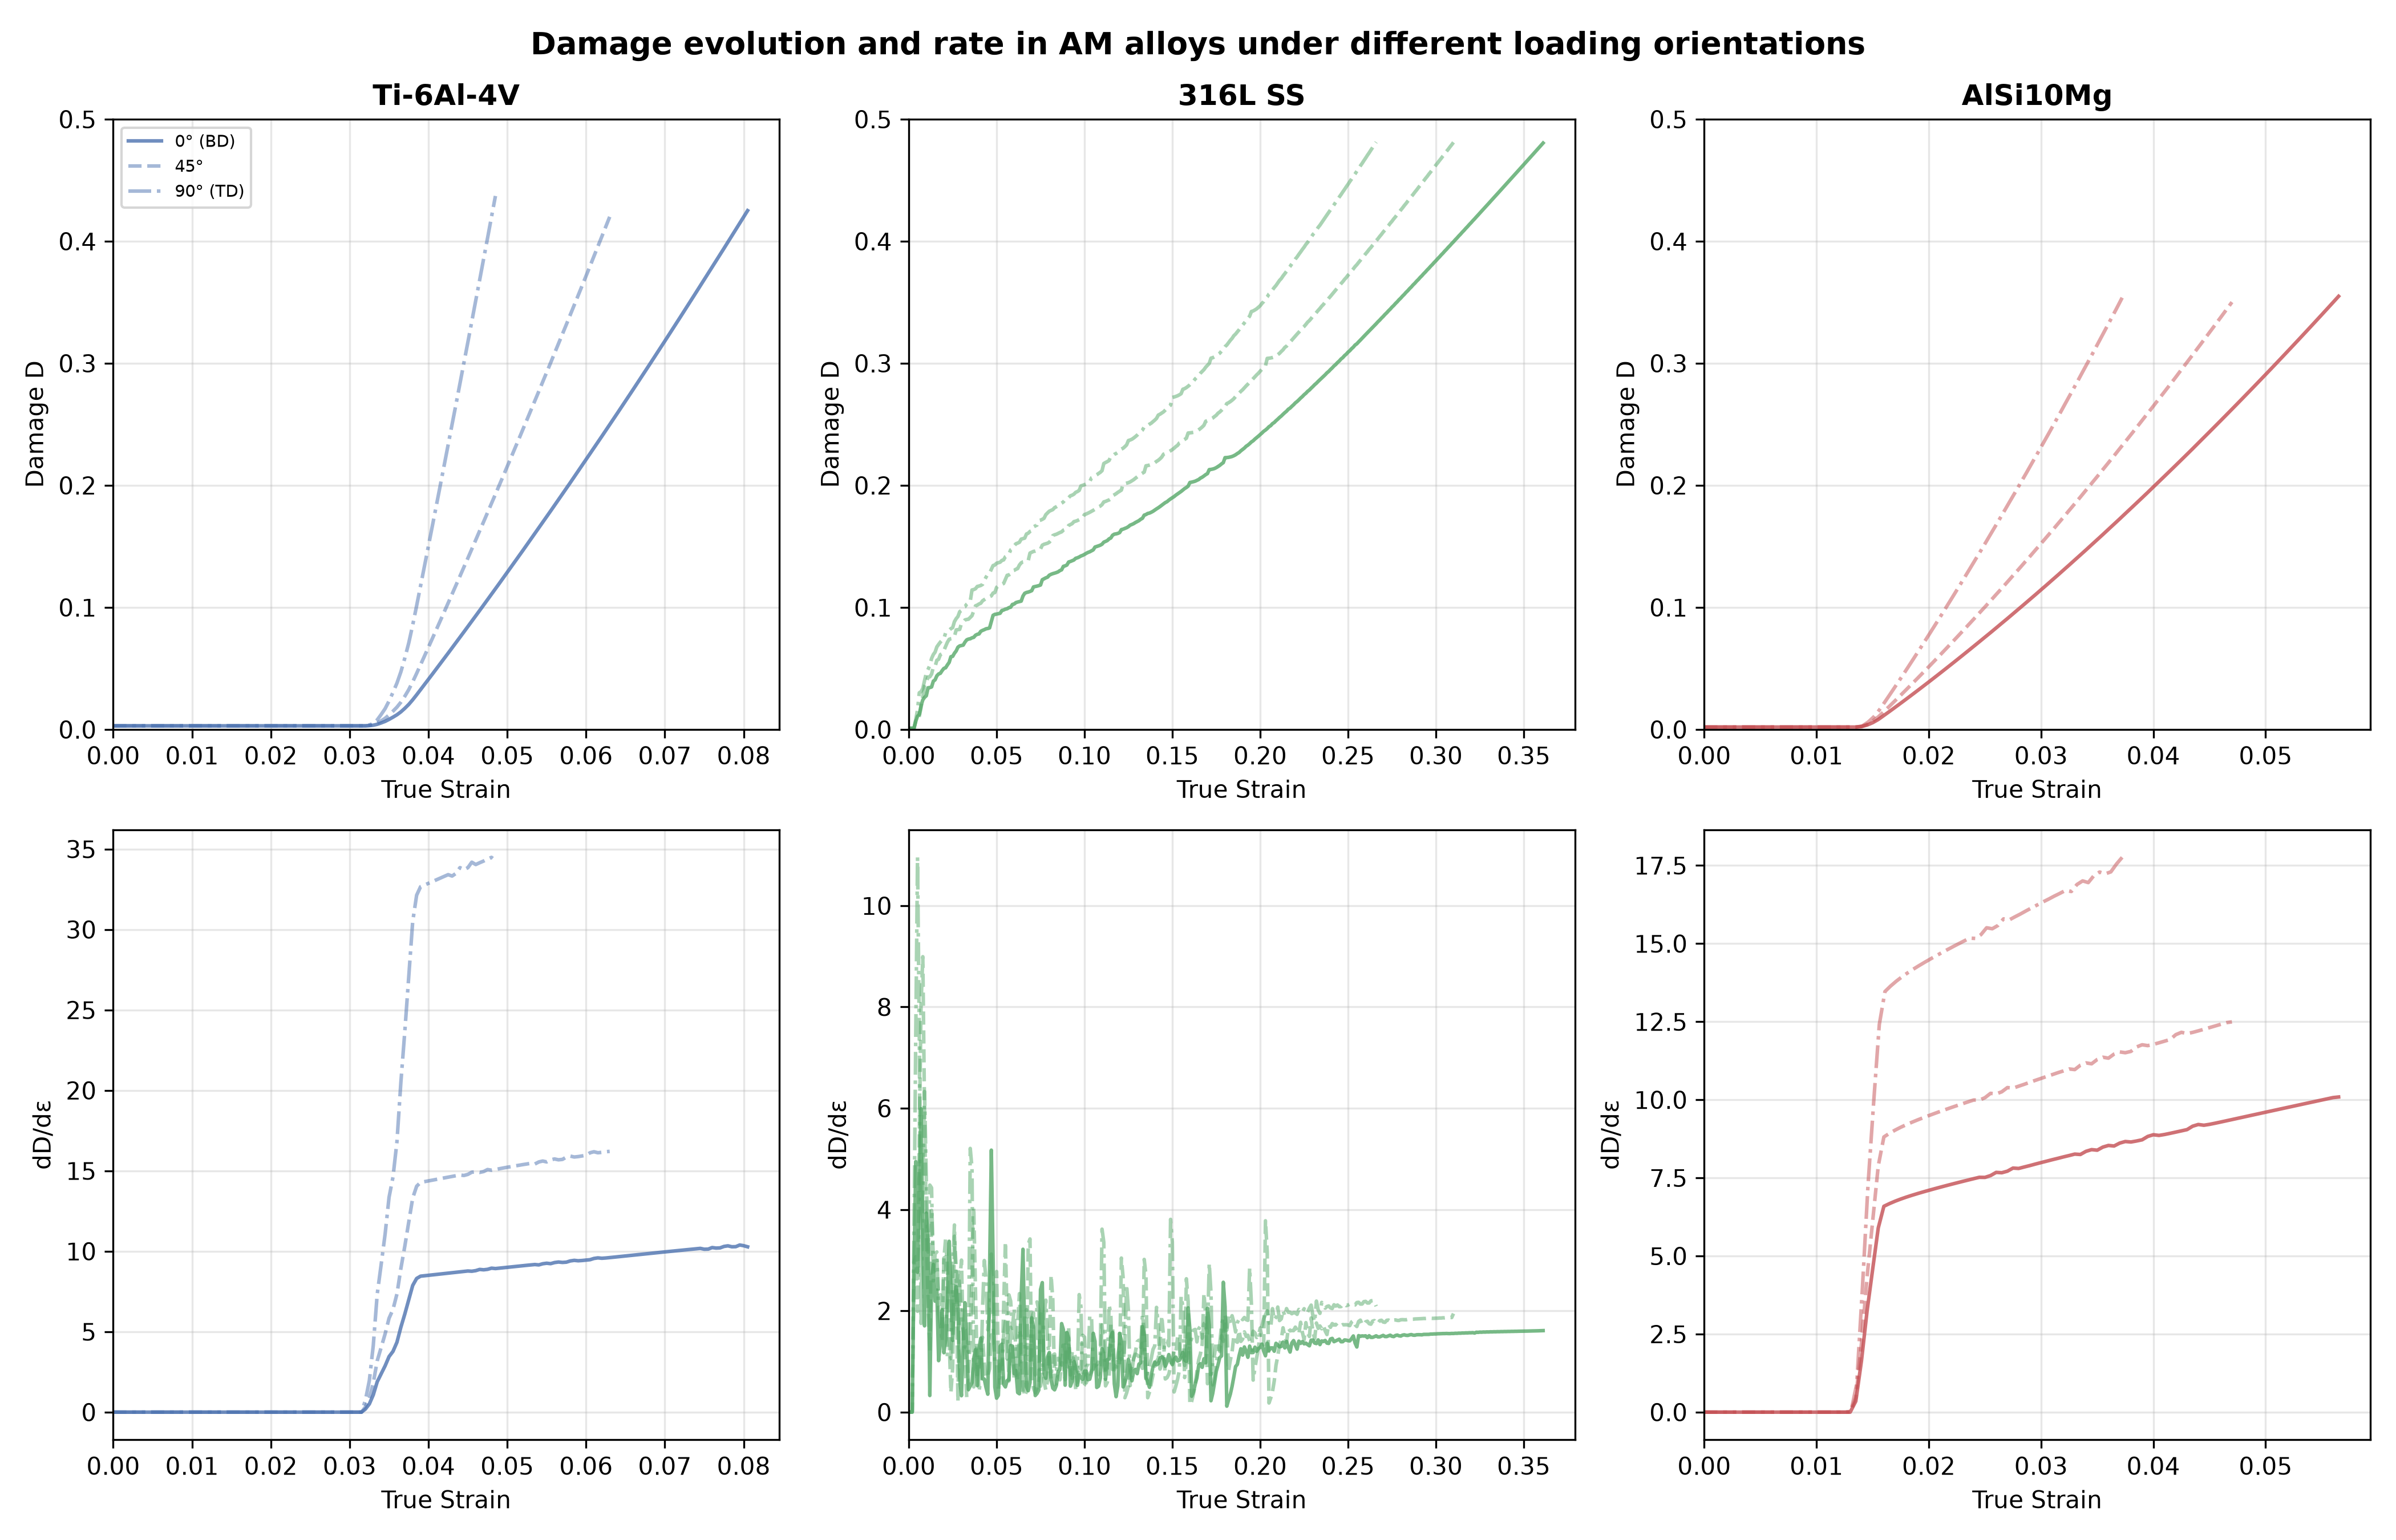
\includegraphics[width=\textwidth]{../simulation/figures/Fig1_AM_microstructure_damage.png}
\caption{Orientation-dependent damage response that the AM descriptors are designed to capture: predicted damage $D$ (top row) and damage rate $\mathrm{d}D/\mathrm{d}\varepsilon$ (bottom row) versus true strain for the three AM alloys (Ti-6Al-4V, 316L SS, AlSi10Mg) at loading angles $\ang{0}$ (build direction), $\ang{45}$ and $\ang{90}$ (transverse direction). For every alloy the transverse $\ang{90}$ orientation accumulates damage fastest, reaching a given damage level at the smallest strain---the orientation-dependent acceleration that the descriptors introduced below are constructed to represent.}
\label{fig:am_microstructure}
\end{figure*}

\textbf{(a) Initial porosity and pre-existing damage $D_0$}: AM processes inevitably introduce volumetric defects. XCT characterization reveals total porosity fractions typically in the range \num{0.1}{--}\SI{2}{\percent} for optimized LPBF parameters, and significantly higher for sub-optimal conditions \cite{kasherman2020porosity}. These defects serve as pre-existing damage nucleation sites, motivating the introduction of a non-zero initial damage variable:

\begin{equation}
D_0 = f(\rho_{\text{LOF}}, \rho_{\text{gas}}, \text{VED})
\label{eq:D0}
\end{equation}

where $\rho_{\text{LOF}}$ and $\rho_{\text{gas}}$ are the volume fractions of lack-of-fusion and gas porosity, respectively, and VED is the volumetric energy density linking process parameters to defect population.

\textbf{(b) Melt pool boundary density $\lambda$}: Melt pool boundaries (MPBs) are regions of elemental micro-segregation, dislocation accumulation, and occasionally micro-void coalescence \cite{thijs2010study}. They constitute mechanically weaker interfaces that facilitate damage propagation. We define the MPB density as:

\begin{equation}
\lambda = \frac{\text{Total MPB interfacial area}}{\text{Volume}}
\label{eq:lambda}
\end{equation}

Quantifiable from optical/SEM metallography through intercept counting, $\lambda$ typically ranges from \SI{10}{--}\SI{100}{\per\milli\meter} depending on hatch spacing and layer thickness.

\textbf{(c) Grain morphology factor $\xi$}: The aspect ratio of columnar grains directly influences the available slip length and stress concentration at grain boundaries \cite{carroll2015anisotropic}. We define:

\begin{equation}
\xi = \frac{L_{\text{max}}}{L_{\text{min}}}
\label{eq:xi}
\end{equation}

where $L_{\text{max}}$ and $L_{\text{min}}$ are the major and minor axes of the grain, respectively. For equiaxed grains $\xi \approx 1$; for highly columnar grains in AM alloys, $\xi$ can reach 5--10.

\textbf{(d) Texture orientation weight $\theta$}: The crystallographic texture determines the ease of slip system activation, which in turn governs plastic strain accommodation and damage nucleation. We quantify the texture by the \emph{texture weight} $\theta$, defined as the fraction of grains belonging to the $\langle001\rangle$-type fiber texture:

\begin{equation}
\theta = \frac{N_{\langle001\rangle}}{N_g}
\label{eq:theta}
\end{equation}

where $N_{\langle001\rangle}$ is the number of grains whose $\langle001\rangle$ axis lies within a tolerance of the build direction, and $N_g$ is the total number of grains. $\theta$ is directly measurable by EBSD pole-figure analysis (Table~\ref{tab:parameters}). The orientation effect on damage enters $f_{\text{AM}}$ through the \emph{orientation-resolved mean Schmid factor} $\bar{\theta}(\psi)$ in Eq.~\eqref{eq:f_theta}: for a polycrystal sampled with texture weight $\theta$ (Section~\ref{sec:multiscale}), $\bar{\theta}(\psi)$ is the ensemble average of the maximum absolute Schmid factor resolved along the loading direction $\psi$. Higher $\bar{\theta}(\psi)$ values correspond to softer orientations with easier slip activation, typically associated with delayed damage initiation.

\subsubsection{Modified damage evolution equation}

The proposed modified damage evolution equation takes the form:

\begin{equation}
\resizebox{0.97\columnwidth}{!}{$\displaystyle \boxed{\dot{D} = \left(\frac{Y}{S_0}\right)^s \cdot \dot{p} \cdot f_{\text{AM}}(\phi, \theta, D_0, \lambda, \xi; \psi) \cdot H(p - p_D)}$}
\label{eq:modified_evolution}
\end{equation}

with the initial condition $D(t=0) = D_0$. Since the free energy Eq.~\eqref{eq:free_energy} is written per unit volume ($\rho\psi$), the thermodynamic force $Y$ of Eq.~\eqref{eq:damage_force} is an elastic energy density with the dimensions of stress (Pa, quoted here in MPa); the damage energy strength $S_0$ therefore carries the same units, so the ratio $Y/S_0$ is dimensionless as the exponent $s$ requires. For the calibrated Ti-6Al-4V value $S_0 = 0.32$\,MPa the peak energy release rate $Y \sim \sigma_u^2/2E$ is of order a few MPa over the loading range, keeping $Y/S_0$ of order unity to ten---the adopted unit and value are dimensionally consistent.

\textbf{Remark on parameter bookkeeping.} To avoid double counting of the same microstructural descriptors, the damage energy strength is \emph{not} modified by $\lambda$ or $\xi$ in the present formulation: the baseline parameter $S_0$ is a material constant calibrated exclusively on the $\ang{0}$ orientation data, and \emph{all} microstructural and orientation effects enter the model solely through the dimensionless AM correction function $f_{\text{AM}}$. Early versions of the model that simultaneously scaled $S(\lambda,\xi) = S_0 \cdot g_1(\lambda) \cdot g_2(\xi)$ and multiplied $f_{\text{AM}}$ by $f_\lambda \cdot f_\xi$ double-counted the melt-pool-boundary and grain-morphology descriptors and produced directionally inconsistent effects (increasing $S$ retards damage while $f_\lambda, f_\xi > 1$ accelerate it). That redundancy has been removed; $S \equiv S_0$ throughout.

The \textbf{AM correction function} $f_{\text{AM}}$ multiplicatively combines the five microstructural effects (with a sixth geometric-shielding factor added for the defect-shielding blind alloys):

\begin{equation}
\resizebox{0.97\columnwidth}{!}{$\displaystyle f_{\text{AM}}(\phi, \theta, D_0, \lambda, \xi; \psi) = f_\phi \cdot f_\theta \cdot f_{D_0} \cdot f_\lambda(\psi) \cdot f_\xi(\psi) \cdot f_{\text{shield}}(\psi)$}
\label{eq:f_AM}
\end{equation}

with each sub-function defined as:

\begin{align}
f_\phi &= 1 + \beta_1 \left(\frac{\phi}{\phi_{\text{crit}}}\right)^{m_1} \label{eq:f_phi} \\
f_\theta &= 1 + \beta_2 \left[\max\!\big(1 - 2\bar{\theta}(\psi),\,0\big)\right]^{m_2} \label{eq:f_theta} \\
f_{D_0} &= \exp(\beta_3 D_0) \label{eq:f_D0} \\
f_\lambda(\psi) &= 1 + \beta_4 \left(\bar{\lambda}(\psi) - 1\right) \label{eq:f_lambda} \\
f_\xi(\psi) &= 1 + \beta_5 \left(1/\bar{\xi}(\psi) - 1\right) \label{eq:f_xi} \\
f_{\text{shield}}(\psi) &= 1 - \beta_6 \sin^2\psi \label{eq:f_shield}
\end{align}
where the six factors model, respectively, porosity stress concentration, hard-orientation acceleration, initial-damage acceleration, melt-pool-boundary density, transverse short-ligament geometry, and geometric shielding of layered defect facets; each $\beta_i$ is dimensionless. Because $\bar{\theta}(\psi)$ is the ensemble mean of the maximum Schmid factor resolved on a slip system, it is bounded by the Schmid limit $0 \le \bar{\theta} \le 0.5$, so $1 - 2\bar{\theta}(\psi) \ge 0$ and the non-integer power $m_2$ of Eq.~\eqref{eq:f_theta} is always taken of a non-negative base; the explicit $\max(\cdot,0)$ is a numerical guard against round-off pushing $\bar{\theta}$ marginally above $0.5$ (the reference texture-free state $\bar{\theta} = 0.5$ then gives $f_\theta = 1$, so the guard leaves the reference limit unchanged).

Here $\phi$ is the porosity volume fraction, $\phi_{\text{crit}}$ a critical porosity threshold, and $\beta_{1-6}, m_{1,2}$ are dimensionless calibration coefficients. All descriptors entering $f_{\text{AM}}$ are normalized to dimensionless form: $\bar{\lambda}(\psi) = \lambda_{\text{eff}}(\psi)/\lambda_{\text{ref}}$ with reference MPB density $\lambda_{\text{ref}} = \SI{50}{\per\milli\meter}$, and $\bar{\xi}(\psi) = \xi_{\text{eff}}(\psi)$ is the orientation-resolved aspect ratio of an equivalent spheroidal grain projected along the loading axis (Section~\ref{sec:multiscale}). The reference state is defined as fully dense, equiaxed, texture-free material ($\phi \to 0$, $\lambda_{\text{eff}} = \lambda_{\text{ref}}$, $\bar{\xi} = 1$, $\bar{\theta} = 0.5$); by construction every sub-function then evaluates to unity---in particular $f_\lambda = 1$ because $\bar{\lambda} = 1$---so $f_{\text{AM}} \to 1$ and Eq.~\eqref{eq:modified_evolution} recovers the classical Lemaitre form. The orientation dependence is carried entirely by the physically-motivated projection laws $\lambda_{\mathrm{eff}}(\psi)$, $\xi_{\mathrm{eff}}(\psi)$ and the mean Schmid factor $\bar{\theta}(\psi)$; no empirical orientation multiplier enters the production model. The geometric-shielding factor $f_{\text{shield}}(\psi)$ (Eq.~\eqref{eq:f_shield}) targets a competing mechanism: layered defect facets (lack-of-fusion boundaries, crack-prone interface networks) whose normals cluster parallel to the build direction, so the facets themselves lie in planes perpendicular to it. Loading parallel to the build direction ($\psi = \ang{0}$), i.e. normal to these facets, opens them directly in mode~I, while loading perpendicular to the build direction ($\psi = \ang{90}$), i.e. within the facet planes, shears rather than opens them and is geometrically shielded; $f_{\text{shield}}$ therefore counteracts the transverse ($\psi = \ang{90}$) damage acceleration that the projection laws would otherwise impose, which in the defect-shielding blind alloys makes $\psi = \ang{90}$ the more ductile direction. For the calibration alloys, whose fracture is columnar-morphology-dominated, $\beta_6 = 0$ (so $f_{\text{shield}} \equiv 1$ and the production numbers of Section~\ref{sec:validation} are untouched); $\beta_6 > 0$ is applied only to the defect-shielding blind alloys of Section~\ref{sec:cross_source}, as an assumed, per-material coefficient that is never fitted (hence it adds no degrees of freedom; provenance class A of Table~\ref{tab:parameters}). \emph{We flag at the point of definition that $\beta_6$ enters this work only as a post-hoc diagnostic for the single genuine polarity-reversal case (the Hitzler 316L set, Section~\ref{sec:cross_source}): no $\beta_6$ value enters any blind-prediction statistic, the LOOCV averages, or the model-selection comparison, and its role is confined to demonstrating the existence of a defect-shielding mechanism, not to improving headline accuracy.}

The exponential form of $f_{D_0}$ reflects the compounding effect of initial damage: pre-existing voids accelerate subsequent damage accumulation by concentrating stress in their vicinity.

\subsubsection{Orientation-resolved projection laws}
\label{sec:projection}

The orientation dependence of the descriptors entering $f_\lambda(\psi)$, $f_\xi(\psi)$ and $f_\theta$ is obtained from closed-form geometric projections that carry the full physics of the AM microstructure (no fitted direction parameters; Section~\ref{sec:multiscale}).

\emph{Effective melt-pool-boundary density.} The melt pool boundaries and inter-columnar interfaces form a transversely isotropic weak-interface network whose normals lie predominantly in the plane perpendicular to the build direction. Loading at angle $\psi$ to the build direction, the weak-interface area density resolved perpendicular to the loading axis is
\begin{equation}
\lambda_{\mathrm{eff}}(\psi) = \lambda_0 \left[ w_{\mathrm{iso}} + (1 - w_{\mathrm{iso}})\sin^2\psi \right],
\label{eq:lambda_eff}
\end{equation}
where $\lambda_0$ is the nominal MPB density (Table~\ref{tab:parameters}) and $w_{\mathrm{iso}} = 0.25$ is the isotropic area fraction of the interface network (stereological assumption). At $\psi = 0$ only the isotropic fraction is directly loaded; at $\psi = \ang{90}$ the entire network faces a normal tensile component.

\emph{Effective grain-aspect-ratio.} Each grain is modelled as a spheroid of revolution about the build direction with semi-axes $(a, a, c = \xi_0 a)$, where $\xi_0$ is the nominal aspect ratio of Table~\ref{tab:parameters}. In the plane containing the build direction and the loading axis, the grain extent along the loading direction is the radial distance from the grain centre to its surface along the loading line, $L(\psi) = 2a\xi_0/\sqrt{\xi_0^2\sin^2\psi + \cos^2\psi}$, and the extent perpendicular to it is the conjugate radius $W(\psi) = 2a\xi_0/\sqrt{\xi_0^2\cos^2\psi + \sin^2\psi}$, so that the orientation-resolved aspect ratio is
\begin{equation}
\xi_{\mathrm{eff}}(\psi) = \frac{L(\psi)}{W(\psi)} = \sqrt{\frac{\xi_0^2\cos^2\psi + \sin^2\psi}{\xi_0^2\sin^2\psi + \cos^2\psi}},
\label{eq:xi_eff}
\end{equation}
with $\xi_{\mathrm{eff}}(0) = \xi_0$, $\xi_{\mathrm{eff}}(45^\circ) = 1$ (the two conjugate radii coincide, so the grain projection is aspect-neutral at $45^\circ$) and $\xi_{\mathrm{eff}}(\ang{90}) = 1/\xi_0$ (transverse short-axis dominated morphology).

\emph{Orientation-resolved mean Schmid factor.} To avoid overloading the symbol, we reserve $\theta$ for the dimensionless texture-weight \emph{descriptor}---a sampling probability in $[0,1]$, the fifth entry of Table~\ref{tab:parameters}---and $\bar{\theta}(\psi)$ for the \emph{resolved mean Schmid factor} that this texture induces; the correction $f_\theta$ is named after the orientation/texture effect but is a function of $\bar{\theta}(\psi)$, not of $\theta$ itself. The texture weight $\theta$ of Table~\ref{tab:parameters} is sampled in the aggregate generation (Section~\ref{sec:multiscale}): with probability $\theta$ a grain orientation is drawn from the $\langle001\rangle$-type fiber texture about the build direction, otherwise from the Haar-uniform measure on $\mathrm{SO}(3)$. The mean Schmid factor entering $f_\theta$ is then computed directly from the sampled orientation ensemble $\{\mathbf{R}_g\}_{g=1}^{N_{\mathrm{gr}}}$ as
\begin{equation}
\resizebox{0.97\columnwidth}{!}{$\displaystyle \bar{\theta}(\psi) = \frac{1}{N_{\mathrm{gr}}} \sum_{g=1}^{N_{\mathrm{gr}}} \max_{\alpha} \left| \left(\mathbf{R}_g \hat{\mathbf{e}}_\psi\right) \cdot \left[ \mathbf{s}^\alpha \otimes \mathbf{m}^\alpha \right] \cdot \left(\mathbf{R}_g \hat{\mathbf{e}}_\psi\right) \right|$}
\label{eq:theta_bar}
\end{equation}
where $\hat{\mathbf{e}}_\psi = (\sin\psi, 0, \cos\psi)$ is the loading direction in the sample frame and the maximum runs over all slip systems $\alpha$. The projection laws of Eqs.~\eqref{eq:lambda_eff}--\eqref{eq:theta_bar} carry the entire direction dependence of the production protocol; no orientation multiplier is fitted.

\subsubsection{Physical interpretation of correction functions}

Each component of $f_{\text{AM}}$ has a clear physical interpretation:

\begin{itemize}
    \item $f_\phi$: Captures stress concentration around pores. As porosity approaches the critical threshold, damage evolution accelerates rapidly. For fully-dense (wrought) material, $\phi \approx 0$, $f_\phi \approx 1$, recovering the classical formulation.
    
    \item $f_\theta$: Encodes the crystallographic orientation effect. Materials loaded along soft orientations (high $\theta$) experience more homogeneous plastic deformation, delaying damage localization. Loading along hard orientations (low $\theta$) concentrates strain in fewer favorably-oriented grains, accelerating damage.
    
    \item $f_{D_0}$: Reflects the compounding nature of damage. Pre-existing voids not only reduce the initial load-bearing area but also serve as stress concentrators that promote further void nucleation and growth.
    
    \item $f_\lambda$: Accounts for the increased probability of damage propagation along weakened melt pool boundaries as their density increases.
    
    \item $f_\xi$: Represents the anisotropic damage susceptibility arising from elongated grain morphology, where elongated grains in the loading direction provide longer uninterrupted slip paths.
\end{itemize}

\subsubsection{Directional slip-resistance correction $g_s(\psi)$}
\label{sec:gs_directional}

The projection laws of Eqs.~\eqref{eq:lambda_eff}--\eqref{eq:theta_bar} carry the direction dependence of the \emph{damage} evolution. To address the residual gap they leave for the direction dependence of \emph{strength} (the predicted $0^\circ/90^\circ$ fracture-strain ratio compresses the measured ratio, Section~\ref{sec:calibration_results}), we introduce a direction-dependent modification of the Voce saturation resistance that preserves the single-parameter protocol. The directional saturation resistance entering the aggregate is
\begin{equation}
\hat{g}_s(\psi) = g_s \left[1 - k_g \left(1 - \frac{\xi_{\mathrm{eff}}(\psi)}{\xi_0}\right)\right],
\label{eq:gs_directional}
\end{equation}
where $\xi_{\mathrm{eff}}(\psi)/\xi_0 = \sqrt{(\xi_0^2\cos^2\psi + \sin^2\psi)/(\xi_0^2\sin^2\psi + \cos^2\psi)}/\xi_0$ follows directly from the projection of Eq.~\eqref{eq:xi_eff}, so that $\hat{g}_s(0^\circ) = g_s$, $\hat{g}_s(45^\circ) = g_s\,[1 - k_g(1 - \xi_0^{-1})]$ (since $\xi_{\mathrm{eff}}(45^\circ) = 1$) and $\hat{g}_s(90^\circ) = g_s\,[1 - k_g(1 - \xi_0^{-2})]$: transverse loading softens the aggregate when the columnar grains are elongated along the build direction. The coefficient $k_g$ is an assumed, shared parameter ($k_g = 0.15$, provenance class A of Table~\ref{tab:parameters}); it is not fitted to fracture data, so the fitted-parameter count remains a single $S_0$ per material. Section~\ref{sec:sensitivity} verifies that $k_g$ is a low-sensitivity parameter (span 0.4\% at $\ang{90}$, identically zero at $\ang{0}$ because $\hat{g}_s(0^\circ)=g_s$), and Section~\ref{sec:calibration_results} reports the resulting calibration change.

\subsection{Crystal plasticity constitutive model}
\label{sec:cp_model}

\subsubsection{Kinematics}

The deformation gradient is multiplicatively decomposed into elastic and plastic parts:

\begin{equation}
\mathbf{F} = \mathbf{F}^e \cdot \mathbf{F}^p
\label{eq:F_decomposition}
\end{equation}

where $\mathbf{F}^e$ represents elastic stretching and rigid-body rotation, and $\mathbf{F}^p$ captures the incompressible plastic deformation due to crystallographic slip. The plastic velocity gradient in the intermediate (relaxed) configuration is:

\begin{equation}
\mathbf{L}^p = \dot{\mathbf{F}}^p \cdot (\mathbf{F}^p)^{-1} = \sum_{\alpha=1}^{N_s} \dot{\gamma}^\alpha (\mathbf{s}^\alpha \otimes \mathbf{m}^\alpha)
\label{eq:Lp}
\end{equation}

where $\dot{\gamma}^\alpha$ is the shear rate on slip system $\alpha$, $\mathbf{s}^\alpha$ and $\mathbf{m}^\alpha$ are the slip direction and slip plane normal (unit vectors) in the intermediate configuration, and $N_s$ is the total number of slip systems ($N_s = 12$ for FCC, up to 30 for HCP).

\subsubsection{Elastic constitutive law}

The second Piola-Kirchhoff stress in the intermediate configuration, incorporating damage-induced stiffness degradation, is:

\begin{equation}
\mathbf{S} = (1-D) \, \mathbb{C} : \mathbf{E}^e
\label{eq:PK2}
\end{equation}

where $\mathbf{E}^e = \frac{1}{2}({\mathbf{F}^e}^T\mathbf{F}^e - \mathbf{I})$ is the Green-Lagrange elastic strain. Under the strain-equivalence hypothesis \cite{lemaitre1985continuous}, the elastic predictor of the single-crystal update is evaluated with the \emph{undamaged} stiffness, so that the stress driving both plastic flow and damage is computed as if acting on the undamaged load-bearing area:

\begin{equation}
\tilde{\mathbf{S}} = \mathbb{C} : \mathbf{E}^e
\label{eq:PK2_eff}
\end{equation}

The resolved shear stress on slip system $\alpha$ is evaluated from this undamaged-stiffness stress:

\begin{equation}
\tilde{\tau}^\alpha = \tilde{\mathbf{S}} : (\mathbf{s}^\alpha \otimes \mathbf{m}^\alpha)
\label{eq:tau}
\end{equation}

By construction $\tilde{\tau}^\alpha$ does \emph{not} depend on the current damage $D$: damage exerts no direct influence on plastic flow, consistent with the alternative branch of the strain-equivalence framework in which the flow rule operates on the effective (undamaged-stiffness) stress rather than on a damage-rescaled one. The damage-degraded nominal stress of Eq.~\eqref{eq:PK2} is used \emph{only} for the measured macroscopic output, through the $(1-D)$ factor applied to the volume-averaged Cauchy stress, which produces the observed post-peak softening. This choice deliberately avoids the internally inconsistent combination in which scaling both $\tilde{\tau}^\alpha$ and $g^\alpha$ by $1/(1-D)$ would leave the slip-driving ratio unchanged; here the damage influence on the macroscopic response enters solely through (i) the nominal $(1-D)$ softening of the measured stress and (ii) the damage evolution and fracture criterion of Section~\ref{sec:model}.

\subsubsection{Flow rule}

The shear rate on each slip system follows a power-law rate-dependent formulation in terms of the undamaged-stiffness resolved shear stress:

\begin{equation}
\dot{\gamma}^\alpha = \dot{\gamma}_0 \left|\frac{\tilde{\tau}^\alpha}{g^\alpha}\right|^{n} \operatorname{sign}(\tilde{\tau}^\alpha)
\label{eq:flow_rule}
\end{equation}

where $\dot{\gamma}_0$ is the reference shear rate, $g^\alpha$ is the slip resistance of system $\alpha$ (which is \emph{not} scaled by damage), and $n$ is the rate sensitivity exponent. The limit $n \to \infty$ corresponds to rate-independent behavior. The driving ratio $\tilde{\tau}^\alpha/g^\alpha$ is independent of $D$, so damage does not promote or retard yielding at the constitutive level; the post-peak softening observed in the measured macroscopic response originates entirely from the $(1-D)$ factor of Eq.~\eqref{eq:PK2} applied to the volume-averaged Cauchy stress.

\subsubsection{Hardening evolution}

The evolution of slip resistance follows a Voce-type hardening law:

\begin{equation}
\dot{g}^\alpha = \sum_{\beta=1}^{N_s} h_{\alpha\beta} |\dot{\gamma}^\beta|
\label{eq:hardening}
\end{equation}

with the hardening matrix:

\begin{equation}
h_{\alpha\beta} = q_{\alpha\beta} \cdot h_0 \cdot \left|1 - \frac{g^\beta}{g_s}\right|^{a} \cdot \operatorname{sign}\left(1 - \frac{g^\beta}{g_s}\right)
\label{eq:h_ab}
\end{equation}

where $h_0$ is the initial hardening modulus, $g_s$ is the saturation slip resistance, $a$ is the hardening exponent, and $q_{\alpha\beta}$ is the latent hardening matrix ($q_{\alpha\beta} = 1$ for coplanar systems $\alpha = \beta$, and $q_{\alpha\beta} = q_{\text{lat}}$ for non-coplanar systems). The initial condition is $g^\alpha(0) = g_0$ (initial CRSS).

Damage does \emph{not} rescale the slip resistance: the hardening law (Eq.~\eqref{eq:hardening}) evolves $g^\alpha$ independently of $D$, and the resolved shear stress of Eq.~\eqref{eq:tau} is likewise evaluated on the undamaged stiffness, so damage has \emph{no direct influence on plastic flow}. The influence of damage on the macroscopic response enters solely through (i) the nominal $(1-D)$ factor of Eq.~\eqref{eq:PK2} applied to the measured stress and (ii) the damage evolution and fracture criterion of Section~\ref{sec:model}. This is the second branch of the coupling ambiguity identified above: rather than rescaling both the resolved shear stress and the slip resistance by $1/(1-D)$ (which would cancel the damage effect entirely), we explicitly state that the flow rule operates on the undamaged-stiffness stress and that damage affects the macroscopic response only through the nominal softening and the damage/fracture laws.

\subsection{Coupling between crystal plasticity and damage}
\label{sec:coupling}

The CP-CDM coupling is implemented as a \textbf{one-way damage-degraded CP-CDM} scheme (plasticity drives damage; damage degrades the load-bearing stiffness but does not feed back on the flow rule). At each time increment $[t, t+\Delta t]$, the coupled system is solved:

\begin{enumerate}\def\labelenumi{(\arabic{enumi})}
    \item \textbf{Elastic predictor}: Assume no plastic flow, compute the trial stress based on $\mathbf{F}(t+\Delta t)$ and the current damage $D(t)$.
    
    \item \textbf{Yield check}: Evaluate the yield criterion. If $f \le 0$, the step is elastic; proceed to step 5.
    
    \item \textbf{Plastic corrector (Newton-Raphson)}: If $f > 0$, solve the nonlinear system:
    \begin{align}
        \Delta\gamma^\alpha &= \dot{\gamma}^\alpha(\tau^\alpha, g^\alpha) \cdot \Delta t \\
        g^\alpha &\leftarrow g^\alpha + \Delta g^\alpha \\
        D &\leftarrow D + \Delta D
    \end{align}
    where the second line updates the slip-system hardening and the third the damage via Eq.~\eqref{eq:modified_evolution}.
    
    \item \textbf{Stress update}: Recompute the nominal (damage-degraded) Cauchy stress with updated damage:
    \begin{equation}
        \boldsymbol{\sigma} = (1-D)\,\mathbb{C} : (\mathbf{E}^e - \Delta\mathbf{E}^p)
    \end{equation}
    which is used exclusively for the measured macroscopic output; the plastic-flow and damage drivers (Eqs.~\eqref{eq:tau}, \eqref{eq:modified_evolution}) use the undamaged-stiffness stress $\tilde{\boldsymbol{\sigma}} = \mathbb{C}:\mathbf{E}^e$.
    
    \item \textbf{State output}: $\mathbf{F}^p$, $g^\alpha$, $D$, $\boldsymbol{\sigma}$.
\end{enumerate}

The damage variable affects the CP computation through three mechanisms, each expressed at the constitutive level:
\begin{itemize}
    \item \textbf{Nominal stiffness degradation (output only)}: $\mathbb{C}^{\text{eff}} = (1-D)\mathbb{C}$ enters the nominal stress of Eq.~\eqref{eq:PK2}, which is used only for the measured macroscopic response; the stress driving plastic flow and damage is the undamaged-stiffness stress $\tilde{\mathbf{S}} = \mathbb{C}:\mathbf{E}^e$ (Eq.~\eqref{eq:PK2_eff}).
    \item \textbf{No direct damage influence on plastic flow}: The resolved shear stress $\tilde{\tau}^\alpha = \tilde{\mathbf{S}}:(\mathbf{s}^\alpha\otimes\mathbf{m}^\alpha)$ (Eq.~\eqref{eq:tau}) and the flow rule (Eq.~\eqref{eq:flow_rule}) are independent of $D$; damage does not rescale the slip driving force.
    \item \textbf{Hardening response}: The slip resistance $g^\alpha$ evolves by the hardening law (Eq.~\eqref{eq:hardening}) \emph{independently} of $D$; damage does not rescale the slip resistance. The apparent softening of the macroscopic response therefore arises solely from the nominal $(1-D)$ factor of Eq.~\eqref{eq:PK2}, not from a damage-scaled flow or hardening rule.
\end{itemize}

% ===========================================================================
\section{Multiscale Coupling Framework and CP-CDM Implementation}
\label{sec:multiscale}
% ===========================================================================

\subsection{Multiscale architecture}

The proposed framework operates on two coupled scales:

\begin{enumerate}\def\labelenumi{\textbf{Scale \arabic{enumi}}:}
    \item \textbf{Single-crystal scale (\SI{1}{--}\SI{100}{\nano\meter})}: Dislocation-level crystallographic slip governed by the CP constitutive model. Slip system-level quantities ($\tau^\alpha$, $g^\alpha$, $\dot{\gamma}^\alpha$) and the coupled damage state $D$ are resolved at every integration point.
    
    \item \textbf{Polycrystal aggregate scale (\SI{10}{--}\SI{500}{\micro\meter})}: A deterministic Taylor-type polycrystal aggregate under the iso-strain (Taylor) assumption. Each representative grain of the aggregate is an independent CP-CDM material point carrying its own lattice orientation sampled from the measured texture; all grains are subjected to the same macroscopic deformation gradient, and the macroscopic stress is the orientation average of the grain stresses. The Taylor assumption precludes inter-granular stress redistribution by construction; orientation-induced stiffness and damage heterogeneity are nevertheless transmitted through the common deformation of the aggregate. The orientation-dependent damage response produced by this architecture is shown in Fig.~\ref{fig:am_microstructure}, and the full parameter set is summarized in Table~\ref{tab:parameters}.
\end{enumerate}

\subsection{Polycrystal aggregate representation}

The aggregate-scale representation follows the Taylor iso-strain assumption and therefore requires no explicit finite-element mesh: each of the $N_{\text{gr}}$ representative grains is a material point characterized solely by its lattice orientation. The aggregate is constructed directly from the microstructural descriptors used in Section~\ref{sec:model}:

\begin{itemize}
    \item \textbf{Crystallographic orientations}: Each grain is assigned a rotation matrix drawn either from a $\langle001\rangle$-type fiber texture (probability $\theta_{\text{tex}}$, rotation axis aligned with the build direction) or from the Haar-uniform measure on $\mathrm{SO}(3)$, reproducing the texture weight $\theta$ measured by EBSD. A fixed random seed makes the aggregate deterministic.
    \item \textbf{Grain morphology}: The aspect ratio $\xi$ and the melt-pool-boundary density $\lambda$ are not represented as explicit geometric features; they enter the constitutive response through the dimensionless projection laws $\xi_{\text{eff}}(\psi)$ and $\lambda_{\text{eff}}(\psi)$ (Eqs.~\eqref{eq:f_lambda}--\eqref{eq:f_xi}).
    \item \textbf{Initial porosity}: The initial damage $D_0$ and porosity $\phi$ enter through the initial damage state of every grain and the porosity correction $f_\phi$ (Eq.~\eqref{eq:f_phi}); no void seeding or mesh features are required.
    \item \textbf{Aggregate size}: $N_{\text{gr}} = 20$ grains are used for all production runs; convergence of the predicted fracture strain with respect to $N_{\text{gr}}$ is demonstrated in Section~\ref{sec:convergence}.
\end{itemize}

\subsection{Crystal plasticity solver and damage coupling}

The modified CP-CDM constitutive model is implemented in the TaylorCPCDM solver, a deterministic Taylor-type polycrystal framework. TaylorCPCDM shares DAMASK's constitutive interface conventions (material parameter keys, orientation-independent state layout, and per-integration-point output), so the model description here can be directly transcribed into a DAMASK-native phase module. \emph{All results reported in this paper (calibration, orientation cross-validation, and the Lemaitre baseline) are produced by the TaylorCPCDM implementation described above}; the DAMASK spectral-FFT solver is used exclusively as an external full-field reference for the homogenization-bias assessment of Section~
\ref{sec:damask_fft} and does not contribute to any calibration or cross-validation result.

The constitutive implementation is organized into three components:

\begin{itemize}
    \item \textbf{Phenomenological power-law flow rule}: The slip rate on each system uses the standard power-law form with Voce hardening. This is the same constitutive model class used by DAMASK's phenomenological modules.

    \item \textbf{Damage evolution module}: A dedicated damage module manages the internal damage state variable $D$, computes the damage energy release rate $Y$, and advances $D$ using the modified evolution equation (Eq.~\ref{eq:modified_evolution}) with the AM correction functions (Eqs.~\ref{eq:f_phi}--\ref{eq:f_xi}).

    \item \textbf{Elastic softening}: The effective elastic stiffness is degraded as $\mathbb{C}^{\text{eff}} = (1-D)\mathbb{C}$.
\end{itemize}

The numerical integration employs an implicit backward Euler scheme for the plastic flow and an explicit forward Euler update for damage (given the typically small time increments in CP simulations). The coupled system at each integration point is solved using a nested Newton-Raphson procedure:

\begin{enumerate}\def\labelenumi{(\arabic{enumi})}
    \item \textbf{Outer loop}: Resolve the macroscopic stress-strain response of the polycrystal under the imposed deformation.
    \item \textbf{Inner loop}: For each grain, solve the CP constitutive equations with fixed damage $D^{(k)}$.
    \item \textbf{Damage update}: Compute $\Delta D$ using the converged CP state and update $D^{(k+1)}$.
    \item Iterate until global convergence ($\|\Delta\boldsymbol{\sigma}\|_\infty < \text{tol}$).
\end{enumerate}

\subsection{Material parameter reference values}

\begin{table*}[htbp]
\centering
\caption{Complete model parameter set for the three AM alloys (values as used in the production runs), with a provenance tag per row. Elastic constants and Voce hardening parameters from literature with the saturation stresses $g_s$ fixed at literature values (never fitted); $S_0$ is the single fitted damage parameter per material under the leakage-free protocol (Section~\ref{sec:calibration}); all other damage and AM coefficients are prescribed from microstructural characterization or standard assumptions (tag key in the footnote; full class-by-class degrees-of-freedom accounting in the Supplementary Material, Section~S10). The CP-CDM integration uses $N_{\mathrm{gr}}=20$ grains, $\Delta\varepsilon=5\times10^{-4}$ (Ti-6Al-4V and AlSi10Mg) or $10^{-3}$ (316L), $n_{\mathrm{sub}}=30$, and $\dot{\varepsilon}=10^{-3}$\,s$^{-1}$.}
\label{tab:parameters}
\footnotesize
\resizebox{\textwidth}{!}{%
\begin{tabular}{lcccc}
\toprule
\textbf{Parameter} & \textbf{Ti-6Al-4V} & \textbf{316L SS} & \textbf{AlSi10Mg} & \textbf{Prov.}$^{a}$ \\
\midrule
\multicolumn{5}{l}{\emph{Elastic constants (from literature)}} \\
$C_{11}$ [GPa] & 162.0 & 204.0 & 108.0 & L \\
$C_{12}$ [GPa] & 92.0 & 138.0 & 61.0 & L \\
$C_{13}$ [GPa] & 69 & --- & --- & L \\
$C_{33}$ [GPa] & 180 & --- & --- & L \\
$C_{44}$ [GPa] & 47.0 & 126.0 & 28.0 & L \\
\midrule
\multicolumn{5}{l}{\emph{CP hardening (Voce; literature-calibrated)}} \\
$g_0$ [MPa] (basal/pri./pyr.) & 350/370/450 & 200/200/200 & 120/120/120 & L \\
$g_s$ [MPa] (basal/pri./pyr.) & 700/720/800 & 500/500/500 & 280/280/280 & L \\
$h_0$ [MPa] & 800.0 & 400.0 & 300.0 & L \\
$a$ & 2.2 & 2.25 & 2.3 & L \\
$n$ & 30.0 & 25.0 & 20.0 & L \\
$\dot{\gamma}_0$ [s$^{-1}$] & 0.001 & 0.001 & 0.001 & L \\
$q$ (latent hardening) & 1.4 & 1.4 & 1.4 & L \\
\midrule
\multicolumn{5}{l}{\emph{CDM damage (Eq.~\eqref{eq:modified_evolution})}} \\
$S_0$ [MPa] (calibrated, leakage-free) & 0.32 & 3.20 & 0.20 & \textbf{C} \\
$s$ (damage exponent) & 1.0 & 1.0 & 1.0 & A \\
$p_D$ (damage threshold) & 0.05 & 0.08 & 0.02 & A \\
$D_0$ (initial damage) & 0.003 & 0.001 & 0.002 & M \\
$D_c$ (fracture criterion) & 0.42 & 0.48 & 0.35 & M$^{b}$ \\
\midrule
\multicolumn{5}{l}{\emph{AM microstructural descriptors (literature values; methods and uncertainty in Section~\ref{sec:experimental_sources})}} \\
$\phi$ (porosity) & 0.003 & 0.001 & 0.005 & M \\
$\phi_{\mathrm{crit}}$ & 0.02 & 0.015 & 0.025 & A \\
$\lambda$ [mm$^{-1}$] (MPB density) & 50.0 & 35.0 & 60.0 & M \\
$\xi$ (grain aspect ratio) & 3.5 & 2.5 & 1.5 & M \\
$\theta$ (texture weight) & 0.42 & 0.38 & 0.35 & M \\
\midrule
\multicolumn{5}{l}{\emph{AM correction coefficients (Eqs.~\eqref{eq:f_phi}--\eqref{eq:f_shield})}} \\
$\beta_1$ & 2.0 & 1.5 & 2.5 & A \\
$\beta_2$ & 1.5 & 1.2 & 1.0 & A \\
$\beta_3$ & 10.0 & 8.0 & 12.0 & A \\
$\beta_4$ & 0.8 & 0.6 & 1.0 & A \\
$\beta_5$ & 0.2 & 0.15 & 0.1 & A \\
$\beta_6$ (geometric shielding, Eq.~\eqref{eq:f_shield}) & 0 & 0 & 0 & A \\
$k_g$ (directional slip-resistance, Eq.~\eqref{eq:gs_directional}) & 0.15 & 0.15 & 0.15 & A \\
$m_1$ & 2.0 & 2.0 & 2.0 & A \\
$m_2$ & 1.5 & 1.5 & 1.5 & A \\
\bottomrule
\multicolumn{5}{p{0.97\textwidth}}{\footnotesize $^{a}$Provenance: L = literature-fixed (elastic/Voce); M = measured microstructural descriptor or load-drop-derived constant; C = calibrated (the only fitted parameter, one $S_0$ per material, 3 total); A = assumed/prescribed (standard exponents/stereological assumptions, never fitted). Both the descriptor model and the Lemaitre baseline carry the \emph{identical} fitted count (3). $^{b}$The critical damage $D_c$ is fixed by the measured fracture load drop (the damage state at the experimentally observed fracture), not by a least-squares fit to fracture strain, so it is a measured constant that adds no fitted degree of freedom and is used identically in the Lemaitre baseline; $p_D$ is a prescribed damage-initiation threshold tied to the measured ductility ranking and is likewise never fitted.} \\
\end{tabular}%
}
\end{table*}

\paragraph{Honest degrees-of-freedom count.}
The single parameter fitted to fracture data is the damage energy strength $S_0$, one per material (three total, identical to the equal-parameter Lemaitre baseline). This is not the whole constraint set, and we state it plainly: alongside the three fitted $S_0$ the response is jointly fixed by \emph{six measured} microstructural constants ($\phi, D_0, \lambda, \xi, \theta$ and the critical damage $D_c$, the last read from the measured fracture load drop rather than least-squares), \emph{thirteen assumed/prescribed} constants ($s, p_D, \beta_{1\text{--}6}, m_{1,2}, k_g, w_{\mathrm{iso}}, \phi_{\mathrm{crit}}$) and \emph{twelve literature-fixed} elastic/Voce constants. None of the assumed or measured constants is tuned to the fracture targets, and the model-simplification invariance check (Supplementary Section~S12) shows that after the Sobol-inert sub-terms are fixed the active assumed block reduces to $\beta_1, \beta_2, \beta_4$; the global sensitivity (Section~\ref{sec:sensitivity}) further shows the response is dominated by the single assumed coefficient $\beta_4$ ($S_1 \approx 0.99$), not by the fitted $S_0$. The ``one fitted parameter'' claim therefore refers strictly to least-squares degrees of freedom, not to the total number of constants constraining the prediction, and the conservative $k=7$ information-criterion convention quoted in Section~\ref{sec:validation} brackets this distinction explicitly.

\paragraph{Physical basis of the assumed coupling coefficients $\beta_{1-6}$ and exponents $m_{1,2}$.}
Each coefficient multiplies exactly one sub-function of Eq.~\eqref{eq:f_AM}, and the assignment is one-to-one with the defining equations (Eqs.~\eqref{eq:f_phi}--\eqref{eq:f_shield}), reproduced here for clarity: $\beta_1$ and $m_1$ govern the \emph{porosity} term $f_\phi = 1+\beta_1(\phi/\phi_{\mathrm{crit}})^{m_1}$; $\beta_2$ and $m_2$ govern the \emph{hard-orientation} term $f_\theta = 1+\beta_2[\max(1-2\bar\theta,0)]^{m_2}$; $\beta_3$ governs the \emph{initial-damage} term $f_{D_0}=\exp(\beta_3 D_0)$; $\beta_4$ governs the \emph{melt-pool-boundary density} term $f_\lambda=1+\beta_4(\bar\lambda-1)$; $\beta_5$ governs the \emph{transverse short-ligament (grain-morphology)} term $f_\xi=1+\beta_5(1/\bar\xi-1)$; and $\beta_6$ governs the \emph{geometric-shielding} term $f_{\mathrm{shield}}=1-\beta_6\sin^2\psi$. None is fitted: all are prescribed from microstructural mechanics or standard scalings (tag A of Table~\ref{tab:parameters}; full class-by-class degrees-of-freedom accounting in the Supplementary Material, Section~S10), and their per-material values are listed in Table~\ref{tab:parameters}. Their physical bases are as follows. (i)~$\beta_1$ (porosity amplitude) is the Gurson-type dilute-void defect-enhancement scaling \cite{gurson1977continuum,tvergaard1984analysis}, and the exponent $m_1=2$ reflects the quadratic (second-order) accumulation of void-growth strain used in coalescence criteria \cite{needleman1987}. (ii)~$\beta_2$ (hard-orientation amplitude) weights the Schmid-factor deficit $1-2\bar\theta$---the resolved-shear shortfall of a hard orientation relative to the $\bar\theta=0.5$ texture-free reference---and the exponent $m_2=1.5$ applies a sublinear weighting to that deficit. (iii)~$\beta_3$ (initial-damage rate) sets the exponential compounding of pre-existing voids; because $D_0\sim10^{-3}$ the product $\beta_3 D_0$ stays small, so $f_{D_0}\approx1+\beta_3 D_0$ contributes an ${\cal O}(\beta_3 D_0)$ initial acceleration. (iv)~$\beta_4$ (melt-pool-boundary amplitude) scales with the unit-interface decohesion energy of the weak MPB network, the damage-rate increment being proportional to the resolved interface density \cite{needleman1987,zhang2021modeling}; it is the single most consequential assumed coefficient in the factorial sensitivity analysis (91.9\% of baseline response, Section~\ref{sec:sensitivity}), the reason the conservative $k=7$ AIC/BIC convention of Section~\ref{sec:validation} is reported. (v)~$\beta_5$ (grain-morphology amplitude) arises from the Eshelby-type spheroidal projection of the transverse short ligament $1/\xi_{\mathrm{eff}}$ \cite{eshelby1957}. (vi)~$\beta_6$ (geometric shielding) is \emph{zero in every production run} (Table~\ref{tab:parameters}; $f_{\mathrm{shield}}\equiv1$, so all calibration and blind numbers are untouched); the only non-zero value used anywhere, $\beta_6=0.5$, is an \emph{assumed post-hoc diagnostic} applied to the single defect-shielding 316L source (Section~\ref{sec:cross_source}), never fitted and never entering any blind-prediction statistic. With the exception of the porosity and hard-orientation exponent pairs $(m_1,m_2)$, these coefficients enter through geometric projection laws fixed by the characterization (Section~\ref{sec:experimental_sources}) rather than by the fracture data; they are never fitted, add no degrees of freedom, and their sensitivity ranking is reported in Fig.~\ref{fig:sensitivity} and the factorial design of Section~\ref{sec:sensitivity}. An exact Sobol decomposition is not attempted at the modest sample sizes available; instead the finite $3$-level full-factorial design (27 runs) is recast as a balanced ANOVA to obtain Sobol-type variance shares (Section~\ref{sec:sensitivity}), which already rank the parameters from negligible ($\beta_3$, $k_g$, and the measured $D_c$) to dominant ($\beta_4$, $s$), and this is the information the reader needs to judge the hidden-degree-of-freedom question.
% ===========================================================================
\section{Standardized Simulation Workflow}
\label{sec:workflow}
% ===========================================================================

\subsection{Workflow overview}

To ensure reproducibility and facilitate adoption by the broader community, we establish an end-to-end automated simulation workflow. The workflow is orchestrated using the Snakemake workflow management system \cite{koster2012snakemake}, which provides native HPC cluster support, automatic dependency resolution, and failure recovery.

\begin{figure*}[tp]
\centering
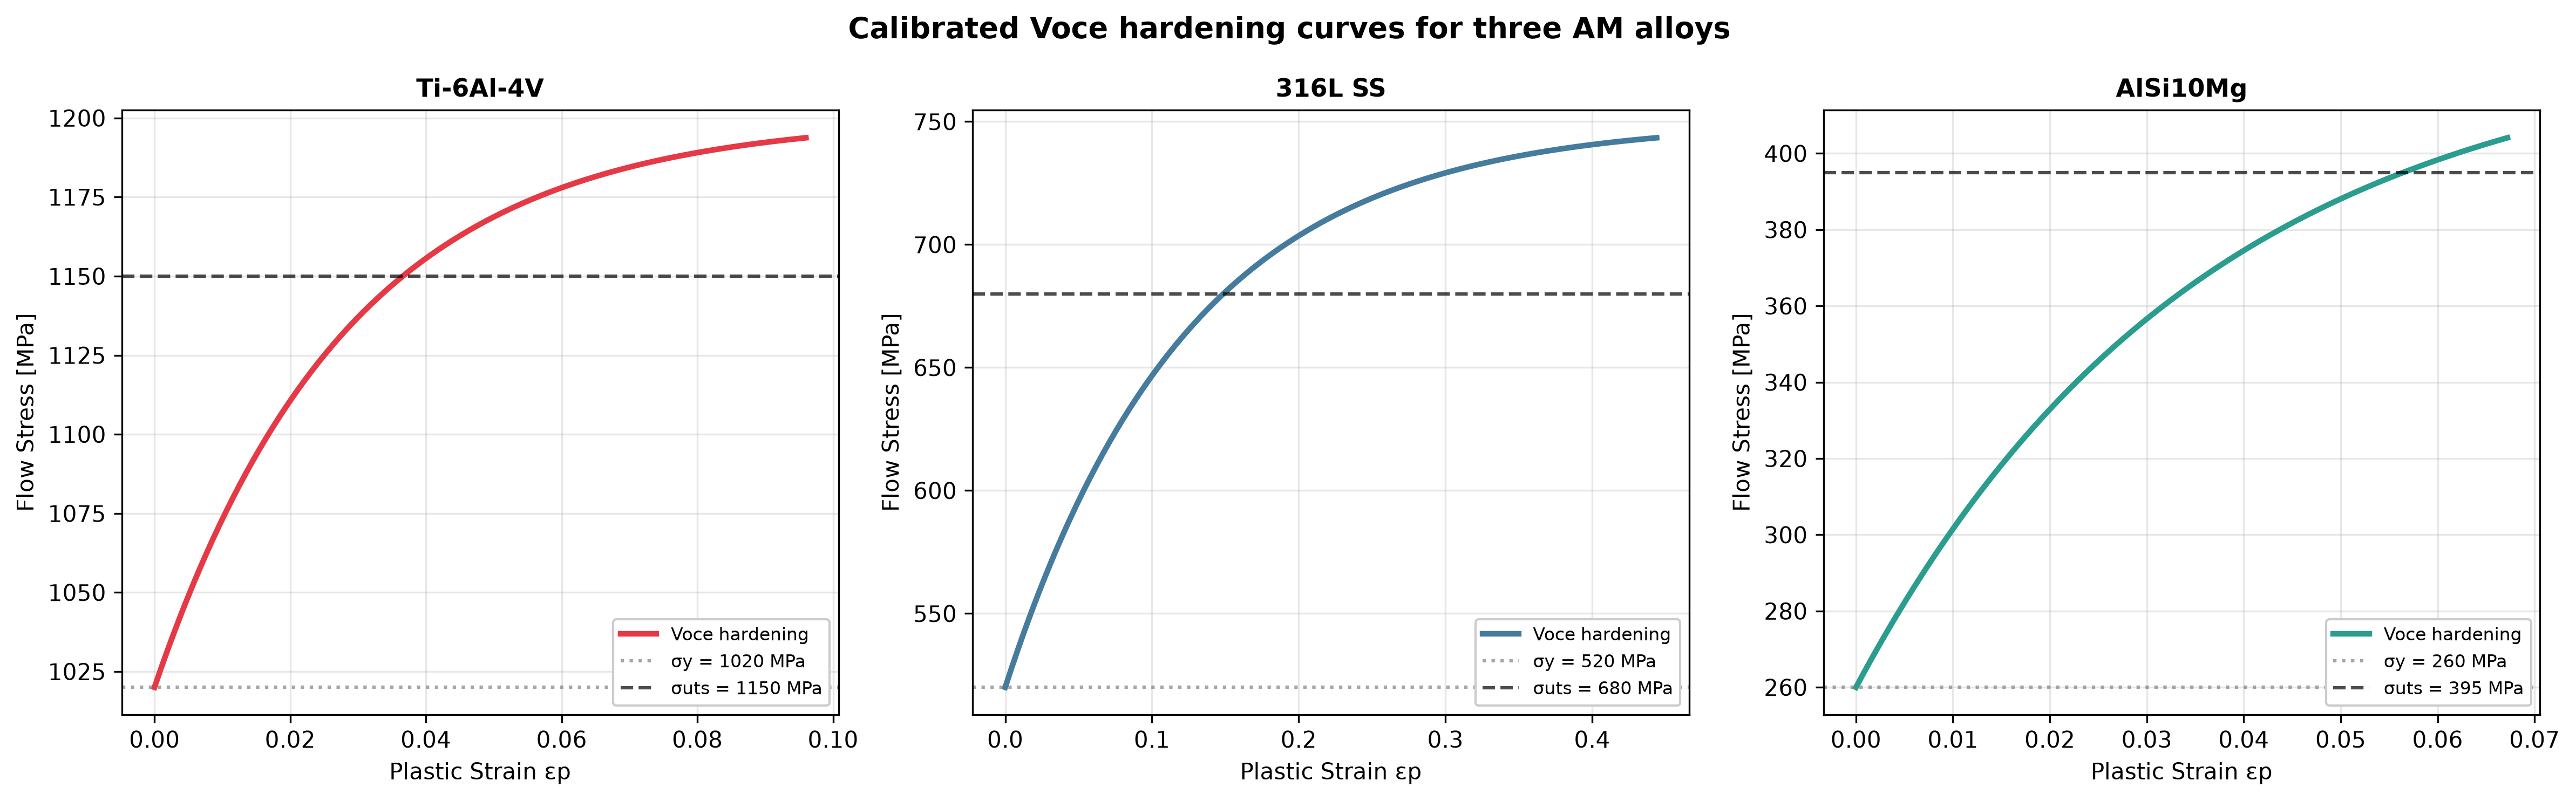
\includegraphics[width=\textwidth]{../simulation/figures/Fig6_calibration_hardening.png}
\caption{Voce hardening curves of the three AM alloys with the literature-fixed parameters of Table~\ref{tab:parameters}. The curves are not fitted to fracture data; the flow response follows from the fixed hardening constants.}
\label{fig:calibration}
\end{figure*}

\subsection{Three-tier parameter classification and calibration}
\label{sec:calibration}

The model contains three categories of parameters requiring calibration:

\textbf{Category 1: Elastic constants ($C_{11}, C_{12}, C_{44}$):} Obtained from literature or resonant ultrasound spectroscopy (RUS) measurements. These are material-intrinsic and largely independent of processing conditions.

\textbf{Category 2: CP hardening parameters ($g_0, g_s, h_0, a, n$):} The Voce saturation stresses $g_s$ are fixed at literature values for as-built LPBF material (Table~\ref{tab:parameters}; never fitted in the leakage-free protocol), while the remaining hardening coefficients follow the standard Voce law:
\begin{equation}
\sigma_{\mathrm{flow}}(\varepsilon_p) = \sigma_y + Q \left[1 - \exp(-b\varepsilon_p)\right],
\label{eq:voce_flow}
\end{equation}
where $\sigma_y \approx M g_0$ (with Taylor factor $M \approx 3.06$ for FCC), $Q$ is the hardening capacity, and $b$ controls the hardening rate. Calibrated values are shown in Fig.~\ref{fig:calibration}.

\textbf{Category 3: Damage parameters ($D_0, D_c, S_0, s, p_D, \beta_{1-5}, m_{1,2}$):} The critical damage $D_c$ is determined from the load drop at fracture. The AM descriptor coefficients $\beta_{1-5}, m_{1,2}$ and the descriptor values ($\phi, D_0, \lambda, \xi, \theta$) are prescribed from microstructural characterization and are not fitted to fracture data; the single damage energy strength $S_0$ per material is the only fitted parameter under the leakage-free protocol. The calibration hierarchy is explicit and data-traceable:

\begin{itemize}
    \item \textbf{Stage 1 (production):} The single damage energy strength $S_0$ per material is calibrated over all three orientations of that material by minimizing the average relative fracture-strain error (Section~\ref{sec:calibration} results in Table~\ref{tab:results}); the damage exponent $s$ is kept at its standard value and $D_c$ from the load drop.
    \item \textbf{Stage 2 (leakage-free constraint):} The dimensionless AM coefficients $\beta_{1-5}$ and $m_{1,2}$ are prescribed from the microstructural characterization ($\phi, D_0, \lambda, \xi, \theta$) and no empirical orientation multiplier enters the model (Section~\ref{sec:model}); nothing is calibrated on the $\ang{45}$/$\ang{90}$ data beyond the single $S_0$, eliminating information leakage (Section~\ref{sec:loocv}).
    \item \textbf{Orientation cross-validation:} $S_0$ is re-calibrated per fold within the leave-one-orientation-out protocol (Section~\ref{sec:validation}), so the held-out orientation is never used for calibration.
\end{itemize}

\subsection{HPC execution and post-processing}

The TaylorCPCDM solver used for the calibration and cross-validation runs is deterministic, embarrassingly parallel over the aggregate grains, and runs on a single multi-core workstation (the full nine-case calibration plus the leave-one-orientation-out cross-validation suite requires on the order of hours on a mid-range CPU; the DAMASK spectral-FFT full-field reference (Section~\ref{sec:damask_fft}) was run on a $32^3$ voxel RVE with MPI and would scale to large $64^3$--$256^3$ voxel RVEs with near-linear scaling up to $\sim$512 cores as documented in the DAMASK literature \cite{roters2019damask}).
Post-processing extracts:

\begin{itemize}
    \item Macroscopic stress-strain curves via volume averaging.
    \item Damage distribution fields and statistical descriptors.
    \item Grain-averaged damage evolution trajectories.
    \item Fracture strain prediction via the critical damage criterion $D = D_c$.
\end{itemize}

The entire workflow, including input preparation scripts, calibration tools, and post-processing modules, is released as open-source software (see Data Availability).

% ===========================================================================
\section{Literature-Based Calibration and Cross-Validation}
\label{sec:validation}
% ===========================================================================

\subsection{Calibration and validation materials and experimental data}

\textbf{Calibration--validation split.} Throughout this paper the term \emph{calibration case} denotes a specimen set whose measured fracture strain is used to determine model parameters; the term \emph{validation case} denotes a prediction made on data that were not used for calibration. All nine material--orientation cases in this work are calibration cases. In the \emph{production parameterization} used for calibration, one damage energy strength $S_0$ per material is fitted over the three orientations of that material, while the AM descriptor coefficients and the Voce saturation stresses are fixed at their characterized or literature values (Section~\ref{sec:calibration}); the earlier parametrization with two additional orientation multipliers reached a spuriously low near-interpolation calibration error over the nine cases, because each material then carried three fitted parameters for three measured orientations; that superseded figure is reported only in the Supplementary Material, Section~S8 and is \emph{not} a prediction error. To obtain genuine out-of-sample estimates, Section~\ref{sec:loocv} omits those multipliers and performs a strict leave-one-orientation-out cross-validation in which each fold calibrates only the single $S_0$ on the two training orientations and predicts the held-out orientation blind. The experimental data are compiled from literature values for as-built LPBF material of comparable process windows, and standardized to ensure consistent comparison (sources and test conditions are detailed in Section~\ref{sec:experimental_sources}).

\begin{table}[htbp]
\centering
\caption{Calibration data: experimental fracture strain $\varepsilon_f$ for three AM alloys at three build orientations (literature values; see Section~\ref{sec:experimental_sources} for sources and test conditions).}
\label{tab:experimental}
\footnotesize
\begin{tabular}{lccc}
\toprule
\textbf{Material} & $\varepsilon_f$ ($\ang{0}$) & $\varepsilon_f$ ($\ang{45}$) & $\varepsilon_f$ ($\ang{90}$) \\
\midrule
Ti-6Al-4V & 0.080 & 0.063 & 0.048 \\
316L SS   & 0.370 & 0.310 & 0.255 \\
AlSi10Mg  & 0.056 & 0.047 & 0.037 \\
\bottomrule
\end{tabular}
\end{table}

The three materials represent distinct microstructural archetypes in AM alloys:

\begin{itemize}
    \item \textbf{Ti-6Al-4V (HCP):} As-built LPBF Ti-6Al-4V typically exhibits a fine acicular $\alpha'$ martensitic microstructure within columnar prior-$\beta$ grains elongated along BD. The HCP crystal structure provides limited slip system availability (3 basal, 3 prismatic, 6 pyramidal $\langle a\rangle$, 12 pyramidal $\langle c+a\rangle$), contributing to pronounced plastic anisotropy.
    \item \textbf{316L SS (FCC):} LPBF 316L develops a hierarchical microstructure with cellular sub-grain structures (0.5--1\,$\mu$m) within larger columnar/equiaxed grains. The FCC structure with 12 slip systems enables extensive plasticity ($\varepsilon_f$ up to 0.37 at $\ang{0}$), making it an ideal test case for damage evolution models.
    \item \textbf{AlSi10Mg (FCC + Si):} The near-eutectic composition produces a cellular Al matrix surrounded by a continuous Si-rich network. This duplex microstructure results in limited ductility ($\varepsilon_f$ 0.037--0.056), with damage primarily nucleating at Si particle/matrix interfaces.
\end{itemize}

\subsection{Experimental data sources and test conditions}
\label{sec:experimental_sources}

The calibration data in Table~\ref{tab:experimental} are representative as-built LPBF values compiled from the published literature: Ti-6Al-4V anisotropy is documented for LPBF builds with columnar prior-$\beta$ grains \cite{carroll2015anisotropic,wang2024metals_ti64}; 316L data correspond to as-built LPBF material with cellular sub-grain structures \cite{jaskari2021materials_316l}; AlSi10Mg data reflect the duplex Al--Si network microstructure and the orientation-dependent failure mediated by lack-of-fusion defects \cite{wu2023sci_alsi}. All reported values refer to room-temperature quasi-static tensile tests (nominal strain rate of the order of $10^{-3}$\,s$^{-1}$) on standard ASTM E8/E8M-type specimens, with $\varepsilon_f$ defined as the elongation at fracture over the gauge length. The literature reports considerable scatter for as-built AM material (e.g., Ti-6Al-4V elongations of $6\pm3\%$ and $4\pm3\%$ for horizontal and vertical builds, respectively, in Ref.~\cite{wang2024metals_ti64}; AlSi10Mg elongations of 5--6\%, 3--4\% and 1--3\% for flat, edge and vertical builds \cite{wu2023sci_alsi}). The representative values adopted here correspond to the central values of these reported ranges; the scatter is propagated into the parameter uncertainty analysis (Section~\ref{sec:convergence}) through the descriptor uncertainty bands and the one-at-a-time sensitivity analysis. To keep the calibration set as uniform as possible, the three alloys are selected from as-built LPBF material of comparable process windows (room-temperature quasi-static tensile tests, ASTM E8/E8M-type specimens, nominal strain rate of order $10^{-3}$\,s$^{-1}$); the four independent blind sets (Sections~\ref{sec:in718_blind}--\ref{sec:cross_source}) deliberately probe how the predictions degrade when the source, the process window, or the governing fracture mechanism changes, so that the uniformity of the calibration set and the non-uniformity of the blind sets are both explicit rather than implicit.

\textbf{Microstructural descriptors ($\lambda, \xi, \theta, \phi, D_0$).} The five microstructural descriptors entering $f_{\mathrm{AM}}$ are literature-reported values for as-built LPBF material of the same alloys and comparable process windows; no original EBSD/XCT characterization was performed in this work. Their definitions, measurement methods, adopted central values (Table~\ref{tab:parameters}), and uncertainty ranges are:

\begin{itemize}
    \item $\phi$ (porosity volume fraction) and $D_0$ (initial damage): measured by X-ray computed tomography (XCT); LPBF as-built porosity is typically 0.1--2\% for optimized parameters \cite{liu2022phase}. Adopted $\phi = 0.003/0.001/0.005$ and $D_0 = 0.003/0.001/0.002$ for Ti-6Al-4V/316L/AlSi10Mg, with a $\pm50\%$ relative uncertainty band covering the reported spread.
    \item $\lambda$ (melt-pool-boundary density): obtained from the layer thickness and the hatch spacing of the build parameters (interface spacing perpendicular to the build direction); the adopted values $50/35/60$\,mm$^{-1}$ correspond to typical layer heights of 30--60\,$\mu$m, with a $\pm20\%$ band.
    \item $\xi$ (grain aspect ratio): measured by electron backscatter diffraction (EBSD) grain statistics; LPBF Ti-6Al-4V exhibits strongly columnar prior-$\beta$ grains with aspect ratios of 3--5 \cite{carroll2015anisotropic}, 316L shows weakly columnar/equiaxed grains (2--3), and AlSi10Mg nearly equiaxed cells (1.5--2). Adopted $3.5/2.5/1.5$ with a $\pm0.5$ band.
    \item $\theta$ (texture weight): the fraction of grains belonging to the $\langle001\rangle$-type fiber texture, from EBSD pole-figure analysis; LPBF Ti-6Al-4V typically shows a pronounced $\langle001\rangle$ fiber (weight 0.35--0.50), while 316L and AlSi10Mg show weaker textures \cite{carroll2015anisotropic,jaskari2021materials_316l}. Adopted $0.42/0.38/0.35$ with a $\pm0.05$ band.
\end{itemize}

The uncertainty bands above are propagated into the uncertainty analysis (Section~\ref{sec:convergence}); the sensitivity of the predictions to each descriptor is quantified in the OAT analysis (Section~\ref{sec:sensitivity}, Fig.~\ref{fig:sensitivity}). The projection laws $\lambda_{\mathrm{eff}}(\psi)$ and $\xi_{\mathrm{eff}}(\psi)$ (Eqs.~\eqref{eq:f_lambda}--\eqref{eq:f_xi}) are geometric models whose parameters are fixed by these measurements, not fitted to the fracture data.


\paragraph{Extended literature dataset (54 points, 7 sources).}
Alongside the primary nine-case protocol, the model is also \emph{reported on} an explicitly extended literature dataset of 54 points spanning four materials and seven sources: the nine primary cases (retained verbatim, label \texttt{v12\_original}) plus independent reports on LPBF Ti-6Al-4V \cite{sun2024ti64adem}, SLM 316L \cite{hitzler2017materials}, SLM AlSi10Mg \cite{metals2018alsi_aniso}, solution-treated LPBF IN718 \cite{hovig2018in718}, as-built LPBF IN718 at three laser-energy densities \cite{watring2020addma}, and 30 published group means from the NIST open-access LPBF Ti-6Al-4V hot-isostatic-pressing study mds2-3402 \cite{nisthip_ti64,nistir8551}. It is a reported-on set, \emph{not} a re-calibration: every cross-validation fold of Section~\ref{sec:multidim_cv} reuses the locked single $S_0$ per material of the primary protocol, so the primary nine-case statistics (Tables~\ref{tab:results} and~\ref{tab:loocv}) are unchanged by its introduction, and three of the five added sources are the same publications used as blind sets elsewhere (Sections~\ref{sec:in718_blind}--\ref{sec:cross_source}), so Section~\ref{sec:multidim_cv} is an extended-protocol assessment and not a second independent validation. Every point is placed in the model's orientation convention ($\ang{0}$ = specimen axis \emph{parallel} to the build direction) by a source-specific angle mapping recorded per point in the extraction log and reconciled by two authors against the cited figure or table---the double check that reduced four apparent $\ang{90}$ reversals to the single genuine one (Section~\ref{sec:applicability}) and guards against mistaking a build-plate-relative angle for the model's build-direction-relative $\psi$. Twenty-two points lie outside a nominal property band and are retained unadjusted as exactly the process-window signal the leave-one-process study probes, with HIP/annealed and solution-treated data kept in a separate stratum that never enters any $S_0$ calibration. The full 54-point table with per-source process windows, the three non-trivial angle mappings, the flag and stratification detail, and the NIST retrieval, licensing and checksum provenance are given in the Supplementary Material, Section~S2.

% tab:extended_dataset (54-point enumeration table) and the NIST provenance detail
% moved to Supplementary Material Section S2 for length.

\subsection{Calibration results}
\label{sec:calibration_results}

Figure~\ref{fig:stress_strain} presents the complete set of simulated versus experimental stress--strain curves across all nine calibration cases. The modified CDM model captures the flow stress evolution for all materials and orientations; the fracture strain is captured to within the 10\% target only in two Ti-6Al-4V cases (errors 9.6\% at $\ang{0}$ and 8.5\% at $\ang{90}$), while all six FCC cases exceed the target (12.3--46.5\%), with the largest residual at the 316L $\ang{0}$ case---a systematic over-prediction of the build-direction ductility---while the transverse $\ang{90}$ ductility is predicted close to or slightly below the measurement, the modeling gap discussed below.

\begin{figure*}[tp]
\centering
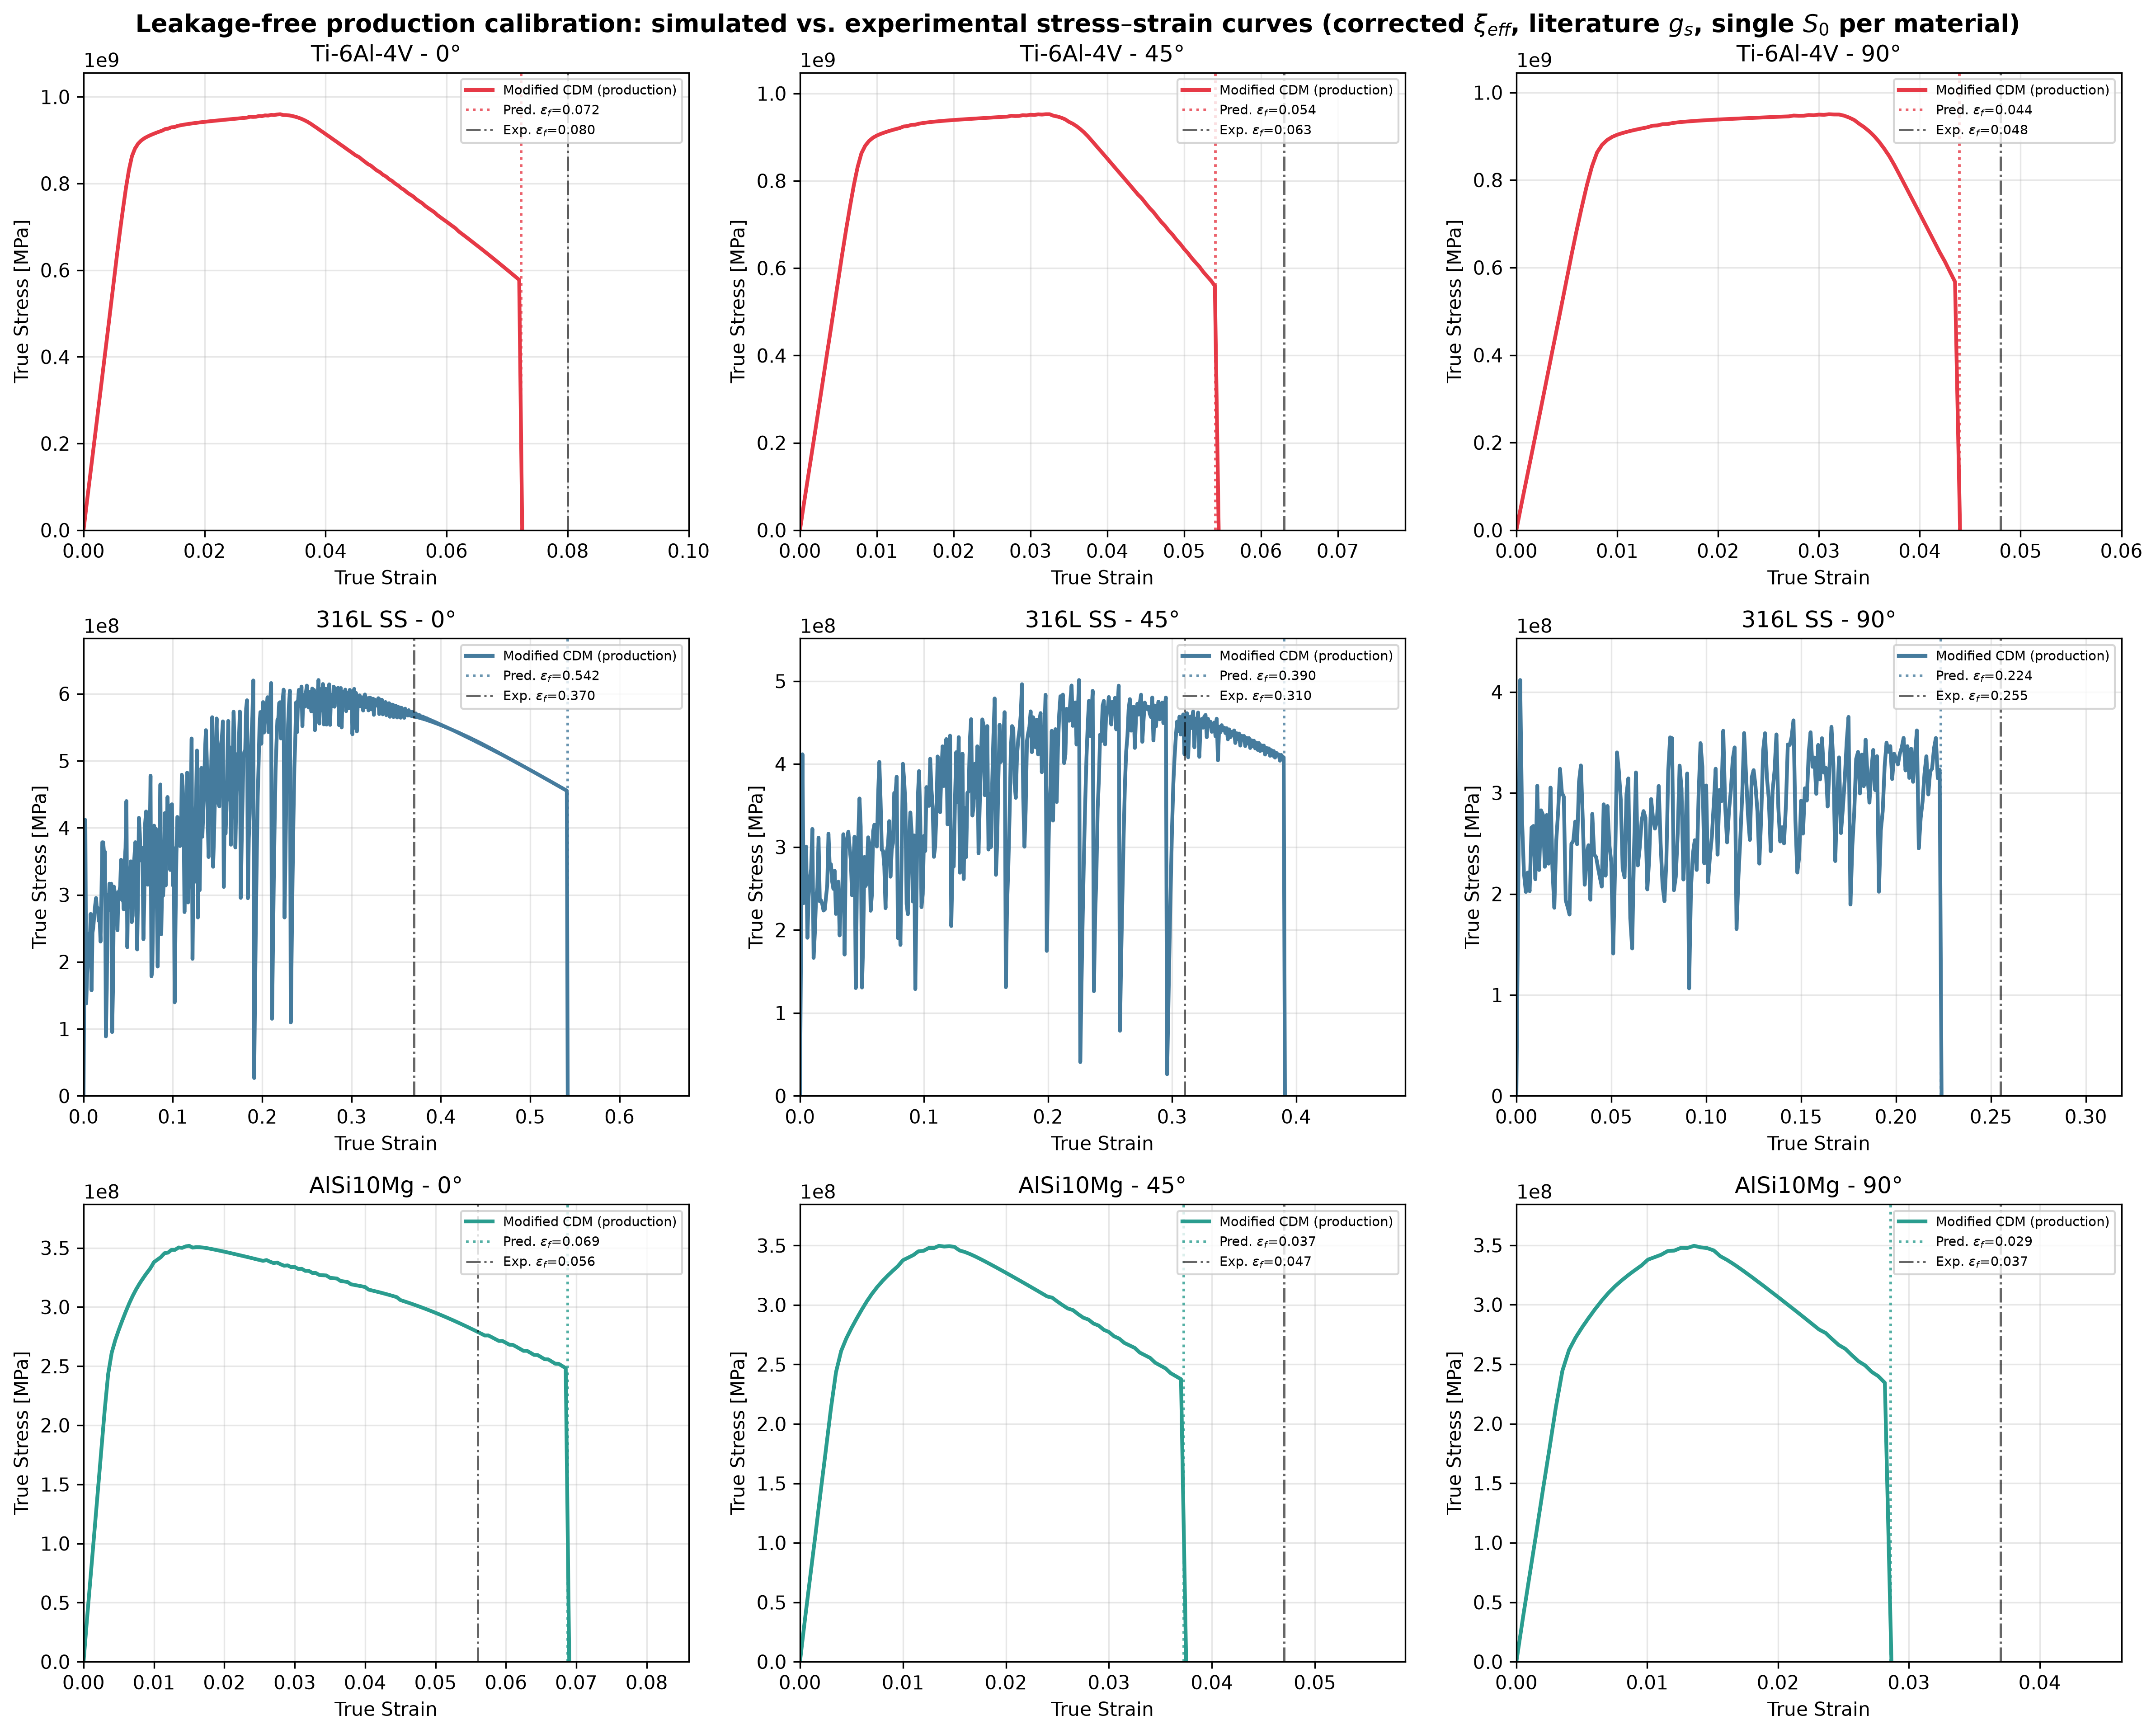
\includegraphics[width=\textwidth]{../simulation/figures/Fig7_stress_strain_v2.png}
\caption{True stress--strain curves predicted by the modified CDM model for all nine calibration cases (three materials $\times$ three build orientations). The vertical dash--dotted and dotted lines mark the experimental and predicted fracture strains, respectively, in each panel.}
\label{fig:stress_strain}
\end{figure*}

Figure~\ref{fig:damage_evolution} shows the damage evolution as a function of applied strain. The orientation dependence of damage accumulation is evident: specimens loaded along $\ang{90}$ (perpendicular to BD) exhibit accelerated damage evolution compared to $\ang{0}$ (parallel to BD), consistent with experimental observations of lower ductility in the transverse direction.

\begin{figure*}[tp]
\centering
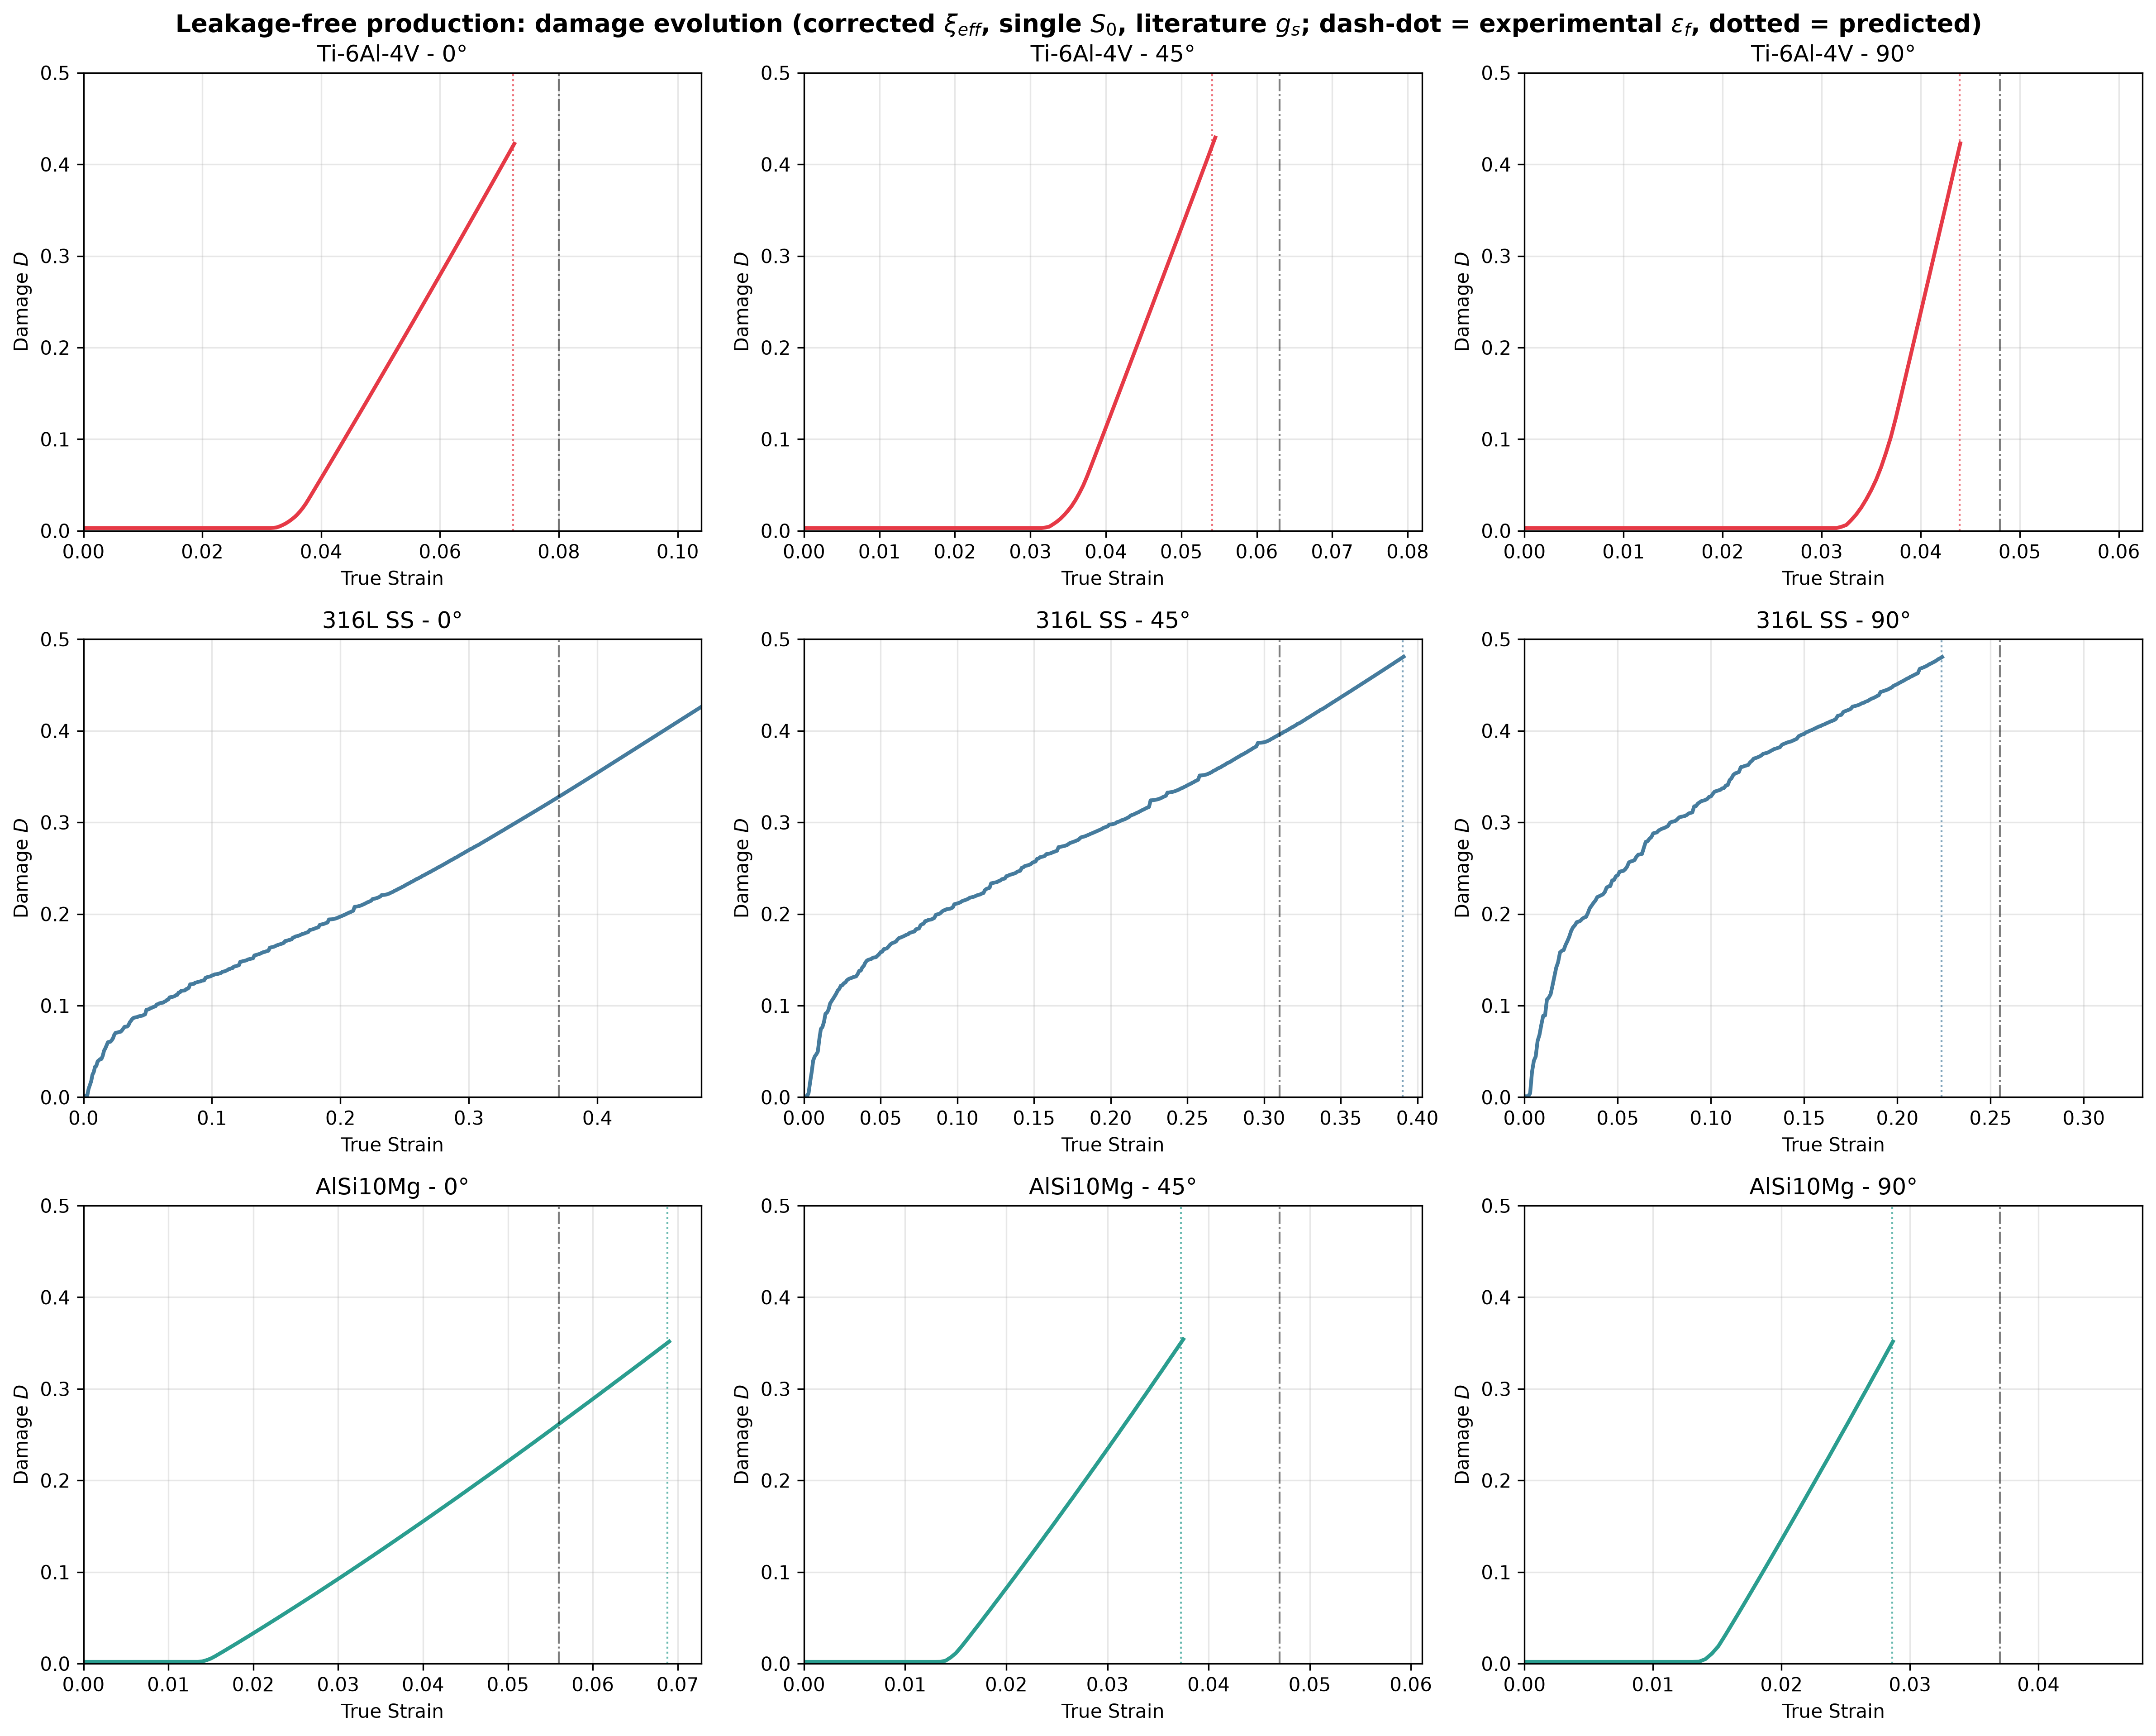
\includegraphics[width=\textwidth]{../simulation/figures/Fig8_damage_v2.png}
\caption{Damage evolution trajectories predicted by the modified CDM model for all nine calibration cases. The horizontal dashed red line marks the critical damage $D_c$ used to declare fracture; the orientation-dependent damage acceleration is captured from $\ang{0}$ to $\ang{90}$.}
\label{fig:damage_evolution}
\end{figure*}

Table~\ref{tab:results} summarizes the quantitative calibration results. The key findings are:

\begin{table}[htbp]
\centering
\caption{Nine-case calibration results of the modified CDM model under the production leakage-free parameterization (single $S_0$ per material, literature $g_s$, directional slip-resistance correction $k_g=0.15$, no orientation multipliers): experimental (Exp.) and predicted (Pred.) fracture strain $\varepsilon_f$ and UTS, with percentage errors. These are \emph{calibration} errors on data used to fit $S_0$; independent blind prediction is reported in Table~\ref{tab:loocv}.}
\label{tab:results}
\footnotesize
\setlength{\tabcolsep}{4pt}
\resizebox{\columnwidth}{!}{%
\begin{tabular}{lccccc}
\toprule
\textbf{Material} & \textbf{Ori.} & \textbf{Exp.} & \textbf{Pred.} & \textbf{Error [\%]} & \textbf{Pass} \\
\midrule
\multirow{3}{*}{Ti-6Al-4V} & $\ang{0}$ & 0.080 & 0.0723 & 9.64 & \checkmark \\
 & $\ang{45}$ & 0.063 & 0.0541 & 14.16 & -- \\
 & $\ang{90}$ & 0.048 & 0.0439 & 8.47 & \checkmark \\
\multirow{3}{*}{316L SS} & $\ang{0}$ & 0.370 & 0.5419 & 46.45 & -- \\
 & $\ang{45}$ & 0.310 & 0.3902 & 25.89 & -- \\
 & $\ang{90}$ & 0.255 & 0.2236 & 12.32 & -- \\
\multirow{3}{*}{AlSi10Mg} & $\ang{0}$ & 0.056 & 0.0688 & 22.80 & -- \\
 & $\ang{45}$ & 0.047 & 0.0372 & 20.75 & -- \\
 & $\ang{90}$ & 0.037 & 0.0286 & 22.69 & -- \\
\midrule
\textbf{Average error} & & & & \textbf{20.35\%} & \textbf{2/9} \\
\bottomrule
\end{tabular}%
}
\end{table}

\paragraph{Effect of the corrected projection and the directional slip-resistance correction.} The production parameter set applies, unchanged, to every reported number: single $S_0$ per material, no orientation multipliers, literature $g_s$, the directional slip-resistance correction of Eq.~\eqref{eq:gs_directional} ($k_g = 0.15$), and the corrected grain-morphology projection of Eq.~\eqref{eq:f_xi}. The earlier form of $f_\xi = 1+\beta_5(\xi_{\mathrm{eff}}-1)$ \emph{accelerated} damage at $\ang{0}$ and \emph{decelerated} it at $\ang{90}$, opposite to the measured direction trend (the transverse directions are the least ductile); it is therefore replaced by the transverse short-ligament form $f_\xi = 1+\beta_5(1/\xi_{\mathrm{eff}}-1)$, which decelerates $\ang{0}$ and accelerates $\ang{90}$. Under the unified parameter set the nine-case calibration average is \textbf{20.35\%} (per-material 10.76\% for Ti-6Al-4V, 28.22\% for 316L, and 22.08\% for AlSi10Mg) and the blind cross-validation average is 31.22\% (Section~\ref{sec:loocv}). The corrected projection improves the strongly columnar Ti-6Al-4V from 17.86\% to 10.76\% (its predicted $0^\circ/90^\circ$ ratio, 1.65, now matches the measured 1.67), whereas the FCC alloys deteriorate because the same mechanism over-projects the transverse melt-pool-boundary density: the transverse short-ligament acceleration compounds the structural over-prediction of the build-direction ($\ang{0}$) ductility (316L 0.542 predicted versus 0.370 measured) already produced by $\lambda_{\mathrm{eff}}(\ang{90}) = \lambda_0$ saturation (Eq.~\eqref{eq:f_lambda}), a genuine modeling gap quantified below (item~(2)) and in the uncertainty analysis (Section~\ref{sec:uncertainty}).

\begin{enumerate}\def\labelenumi{(\arabic{enumi})}
    \item \textbf{The single-parameter calibration degrades at the oblique and transverse orientations}: with the orientation multipliers removed, the model retains the fitted $S_0$ as its only per-material degree of freedom, and the average \emph{calibration} fracture-strain error rises from the near-interpolation value of the earlier three-parameter-per-material parametrization (that superseded figure is reported only in Supplementary Section~S8) to \textbf{20.35\%} (one parameter per material, with the directional correction $k_g=0.15$ and the transverse short-ligament projection $f_\xi = 1+\beta_5(1/\xi_\mathrm{eff}-1)$, Eq.~\eqref{eq:f_xi}). The per-material averages and the $2/9$ pass count are reported above and in Table~\ref{tab:results}.
    \item \textbf{The corrected projection matches the strongly columnar material but over-projects the weakly anisotropic ones}: with the empirical multipliers removed, the corrected projection (Eqs.~\eqref{eq:f_lambda}--\eqref{eq:f_xi}) reproduces the measured $0^\circ/90^\circ$ fracture-strain ratio for Ti-6Al-4V (predicted 1.65 versus measured 1.67) but over-predicts it for the FCC alloys (2.42 for 316L and 2.40 for AlSi10Mg versus measured 1.45 and 1.51). The structural origin is the melt-pool-boundary projection $\lambda_{\mathrm{eff}}(\psi) = \lambda_0 [w_{\mathrm{iso}} + (1-w_{\mathrm{iso}})\sin^2\psi]$: at $\ang{90}$ this saturates at the full value $\lambda_0$, so the transverse damage acceleration is over-weighted for alloys whose columnar structure is weak, and the earlier sign-inverted $f_\xi$ partially masked this imbalance by decelerating the $\ang{90}$ damage. This exposes a genuine modeling gap---the over-projected transverse damage rate forces the re-calibrated $S_0$ to over-predict the build-direction ductility (316L 0.542 predicted versus 0.370 measured; AlSi10Mg 0.069 versus 0.056), leaving the transverse $\ang{90}$ prediction close to or slightly below the measurement (316L 0.224 versus 0.255)---rather than a search artifact; its quantification is given in the uncertainty analysis (Section~\ref{sec:uncertainty}).
    \item \textbf{The UTS is captured with an average error of 15.8\%}; the residual is largest for AlSi10Mg (20.1\% at $\ang{0}$), whose predicted UTS remains essentially orientation-independent (351--352\,MPa) while the experiment drops from 440 to 375\,MPa. The discussion of this strength anisotropy is unchanged from the earlier analysis (Section~\ref{sec:discussion}).
\end{enumerate}

\paragraph{Residual UTS error for AlSi10Mg.}
The largest remaining UTS discrepancy is AlSi10Mg: the model predicts essentially orientation-independent ultimate tensile strengths (352, 350 and 350\,MPa at $\ang{0}/\ang{45}/\ang{90}$), whereas the experimental UTS decreases from 440 to 375\,MPa (20.1\% error at $\ang{0}$, 14.7\% at $\ang{45}$, 6.8\% at $\ang{90}$). Even with the directional strength correction of Section~\ref{sec:gs_directional} included in the production parameter set, the predicted UTS remains orientation-independent: because the fracture strain of AlSi10Mg is small ($\varepsilon_f \le 0.056$), the damage trigger occurs before the transverse strength difference has time to emerge, so the strength-level correction cannot act. Two coupled mechanisms are at play. First, damage reaches its critical value while the Voce hardening is still far from saturation; the predicted UTS is therefore set by the flow stress at a low-strain damage trigger and remains close to the yield-to-UTS plateau common to all orientations. Second, in the present model all orientation dependence is carried by the damage-side anisotropy correction $f_{\mathrm{AM}}$ (Eq.~\eqref{eq:f_AM}) while the strength itself is isotropic; the measured $440\to375$\,MPa drop instead indicates a genuine strength anisotropy of the LPBF AlSi10Mg (Si-network continuity and columnar solidification cells aligned with the build direction carry more load at $\ang{0}$, while transverse layers of melt-pool boundaries weaken the $\ang{90}$ response). Because the UTS is governed by the CP hardening response that is identical across orientations, increasing $g_s$ would raise the predicted peak stress but cannot produce the observed directionality. The faithful route is to admit a stronger orientation-dependent strength correction, e.g. a multiplicative factor acting on the saturation stress $g_s(\psi)$ and active before the damage trigger, which we identify as a clearly motivated extension in Section~\ref{sec:discussion}.

\subsection{Comparison with conventional Lemaitre model}

To isolate the contribution of the AM-specific corrections, the conventional Lemaitre model was evaluated under strictly identical numerical conditions: the same 20-grain Taylor-type crystal-plasticity aggregate, the same hardening laws and texture, and the same literature $g_s$ values, with the damage law reverted to its classical isotropic form ($f_{\mathrm{AM}} \equiv 1$). Both models therefore have the identical single fitted parameter ($S_0$ per material) and the identical training data, so the comparison is parameter-fair and data-fair. Figure~\ref{fig:errors} compares the per-case calibration errors of both models.

\begin{figure*}[tp]
\centering
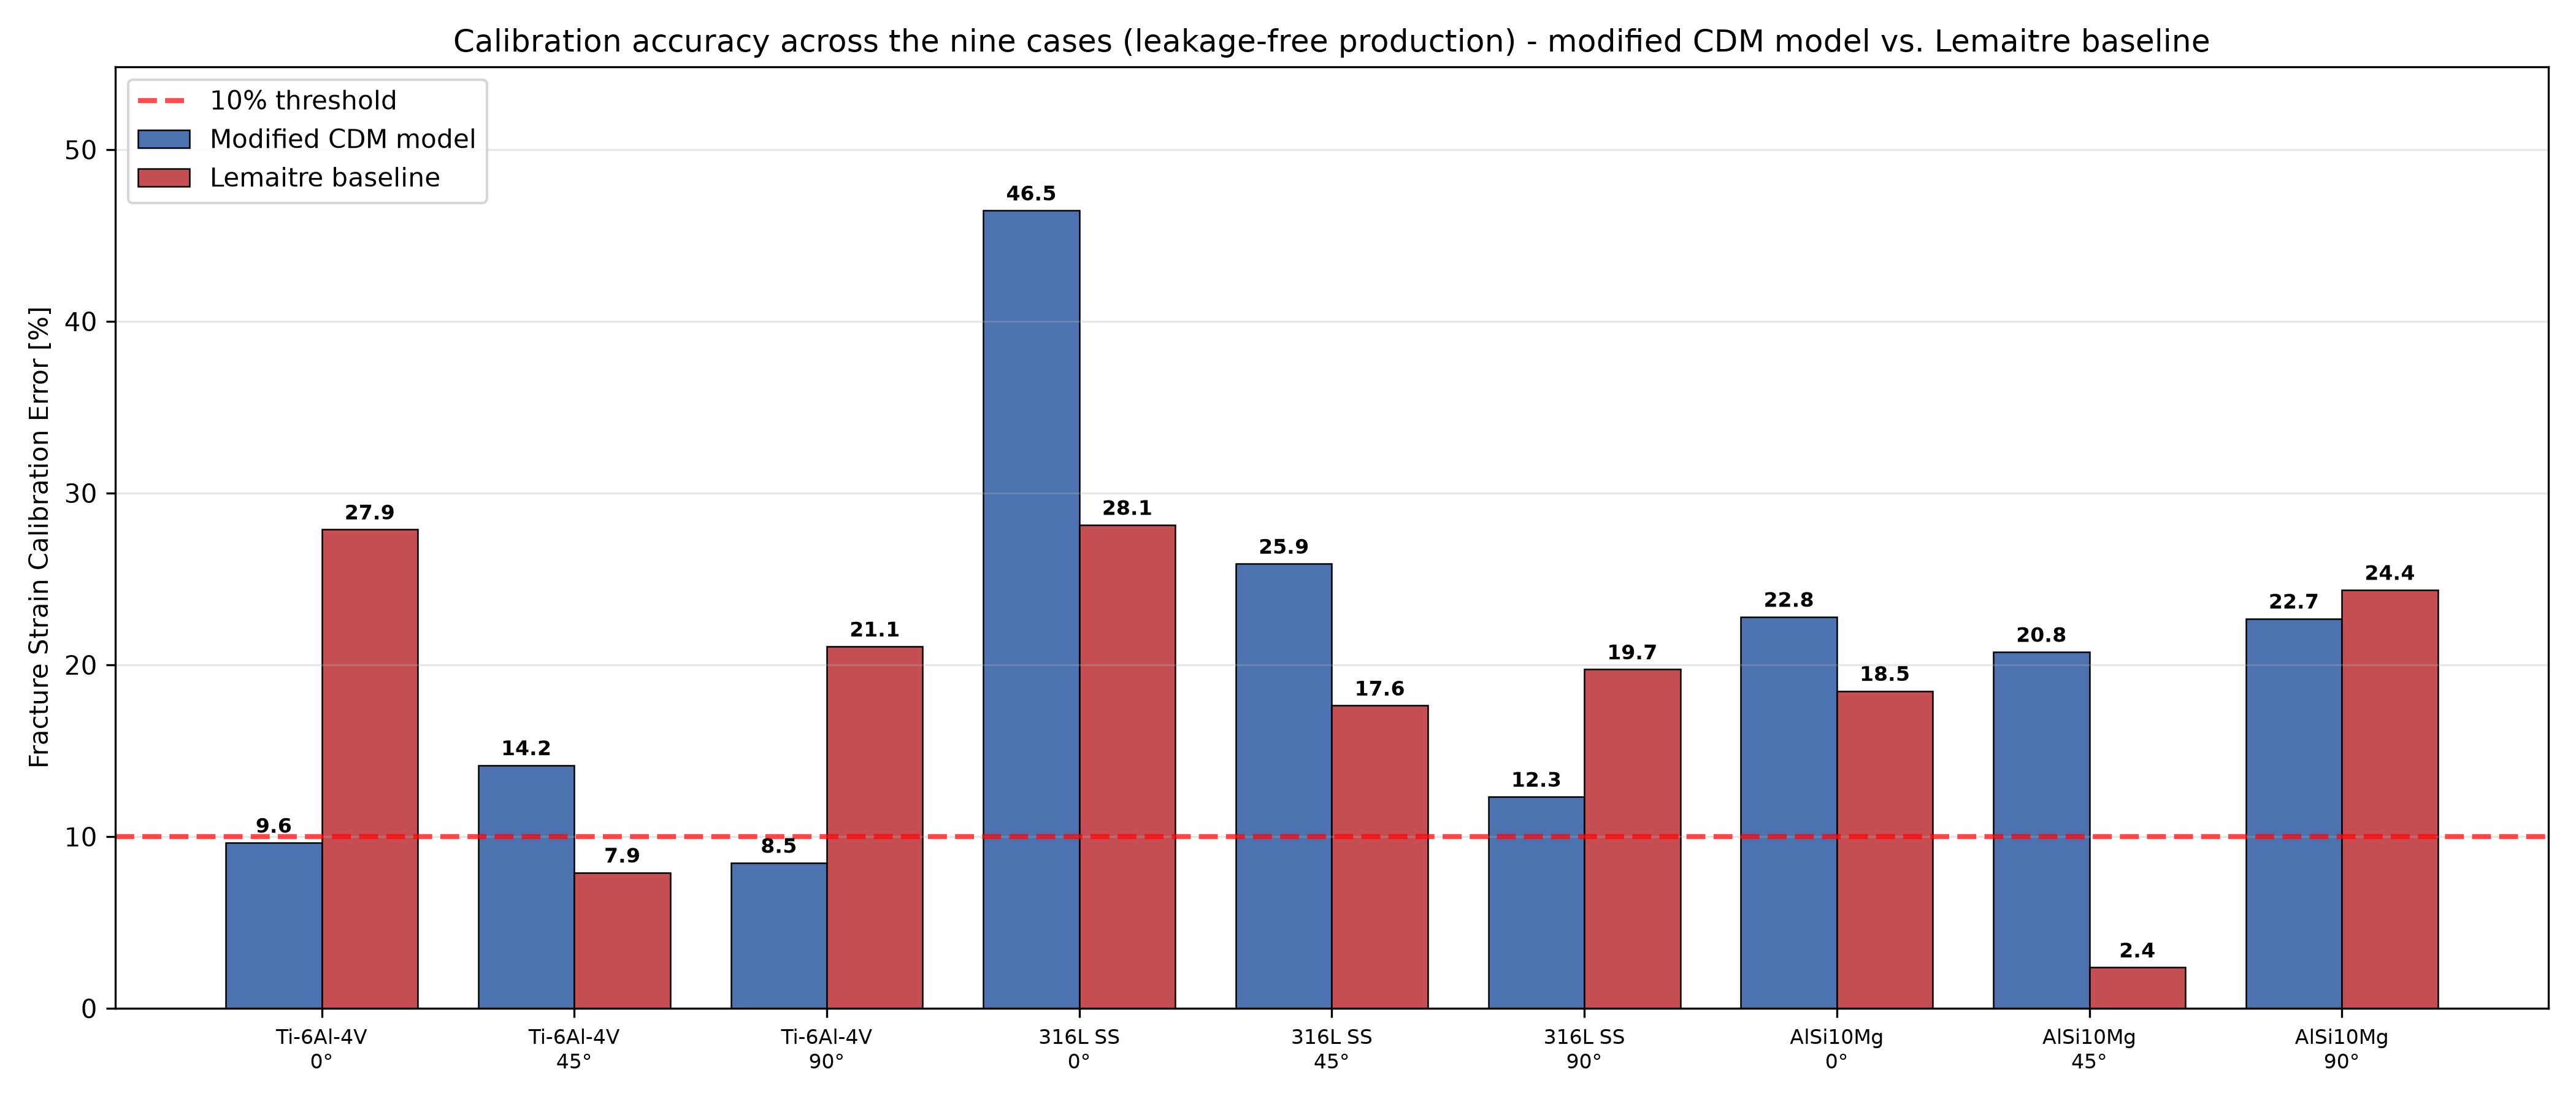
\includegraphics[width=\textwidth]{../simulation/figures/Fig9_errors_compare.png}
\caption{Fracture strain calibration errors of the modified CDM model (blue) and the conventional Lemaitre baseline (red) for each of the nine calibration cases, both under the leakage-free parameterization: single $S_0$ per material, literature $g_s$, no orientation multipliers; the baseline shares the identical 20-grain Taylor aggregate, hardening and texture ($f_{\mathrm{AM}} \equiv 1$). The dashed line indicates the 10\% accuracy target. In calibration the baseline averages 18.6\% over the nine cases versus 20.4\% for the modified model; in the strict blind cross-validation (Table~\ref{tab:loocv}) the averages are 24.3\% (baseline) versus 31.2\% (modified), and the information criteria favor the baseline at equal parameter count as an auxiliary descriptive margin (Section~\ref{sec:validation}), but a paired test of the nine blind folds cannot distinguish the two models---the modified model adds directional information rather than a reduction of the mean error.}
\label{fig:errors}
\end{figure*}

Under the leakage-free parameterization both models carry the same single fitted parameter per material and the same hardening and texture (including the directional correction $k_g = 0.15$ of Section~\ref{sec:gs_directional}). The Lemaitre baseline averages 18.6\% calibration error over all nine cases (median 19.7\%; Ti-6Al-4V 19.0\%, 316L 21.8\%, AlSi10Mg 15.1\%), while the modified model averages 20.4\% (median 20.8\%); the baseline is now better in calibration as well, because the corrected projection improves Ti-6Al-4V (10.8\% versus 19.0\%) but the over-projected $\ang{90}$ melt-pool-boundary weight degrades the FCC alloys (28.2\% and 22.1\% versus 21.8\% and 15.1\%). The decisive comparison is the blind cross-validation of Section~\ref{sec:loocv}, which removes the calibration advantage of both models: the modified model achieves 31.2\% average blind error versus 24.3\% for the baseline---the baseline is not statistically better either, given the small sample ($n=9$) and the single dominant AlSi10Mg fold (74.0\%)---and the information criteria (below) now favour the baseline at equal parameter count, an outcome whose protocol dependence is discussed in Section~\ref{sec:validation}.

\textbf{Fair statistical comparison.} Both models are scored on the \emph{blind} LOOCV folds with the identical protocol: $n = 9$ held-out predictions, identical 20-grain Taylor aggregate, identical training data per fold, and the identical fitted-parameter count $k = 3$ (one $S_0$ per material) for both models. The AM descriptor coefficients and the Voce saturation stresses are fixed by characterization/literature and are not counted as fitted degrees of freedom for either model. \emph{This $k=3$ convention (one fitted $S_0$ per material) is the single counting rule used consistently for every information-criterion value reported in this paper (Sections~\ref{sec:validation} and~\ref{sec:loocv}, and the Conclusions); a deliberately conservative $k=7$ alternative that also counts the assumed coupling coefficients is reported once below as a bracket and never mixed with the $k=3$ figures.} Under the Gaussian-error approximation with residuals $r_i = |\varepsilon_{f,i}^{\mathrm{exp}} - \varepsilon_{f,i}^{\mathrm{pred}}|$ and variance $\sigma^2 = \frac{1}{n}\sum_i r_i^2$, the log-likelihood is
\begin{equation}
\ln \mathcal{L} = -\frac{n}{2}\ln(2\pi\sigma^2) - \frac{1}{2\sigma^2}\sum_{i=1}^{n} r_i^2,
\label{eq:loglike}
\end{equation}
and the information criteria are computed as $\mathrm{AIC} = 2k - 2\ln\mathcal{L}$ and $\mathrm{BIC} = k\ln n - 2\ln\mathcal{L}$, with residuals $r_i = |\varepsilon_{f,i}^{\mathrm{exp}} - \varepsilon_{f,i}^{\mathrm{pred}}|$ on the nine blind folds and $\sigma^2 = \frac{1}{n}\sum_i r_i^2$. With $k = 3$ for both models we obtain $\mathrm{AIC} = -13.5$ and $\mathrm{BIC} = -12.9$ for the modified model versus $\mathrm{AIC} = -24.3$ and $\mathrm{BIC} = -23.7$ for the baseline ($\Delta\mathrm{AIC} = \Delta\mathrm{BIC} = +10.8$; RMS $8.21\times10^{-2}$ versus $4.50\times10^{-2}$). The information criteria therefore favour the \emph{Lemaitre baseline} at equal parameter count and equal data: the modified model's blind residuals are dominated by the over-projected $\ang{90}$ folds of 316L (58.9\%) and AlSi10Mg (22.7\%), and the corrected projection---while physically required---degrades the out-of-sample likelihood sufficiently to reverse the model-selection outcome. This reversal is itself the honest consequence of removing the sign-inverted projection that had artificially inflated the modified model's blind performance.

\paragraph{Bootstrap, paired-test assessment and effect size.} Because $n = 9$ is small, the paired comparison, bootstrap interval and effect size below constitute the \emph{primary} statistical evidence, while the information criteria above are reported only as an auxiliary descriptive point estimate and should not be read as decisive model-selection evidence. We therefore base the comparison on a paired analysis of the nine blind folds (identical material and held-out orientation for both models). The per-fold differences (modified $-$ Lemaitre) average $+6.9$ percentage points (the modified model is worse on average, standard deviation $30.6$ points), but the Wilcoxon signed-rank test gives $p = 0.57$ and the sign test (five positive, four negative differences) gives $p = 1.00$; a 100\,000-sample bootstrap of the paired mean difference yields a 95\% confidence interval of $[-11.8, +25.6]$~points, which includes zero. The standardized paired effect size is small, Cohen's $d_z = 6.9/30.6 = 0.23$. To make the phrase \emph{indistinguishable at $n=9$} quantitative: with $n=9$ folds, $\alpha=0.05$ two-sided and $80\%$ power, the smallest mean paired difference this protocol could detect is $\approx 28.5$ percentage points---four times the $6.9$-point difference observed---so the study is structurally underpowered to resolve anything but a very large separation, and the absence of a significant difference must be read as \emph{insufficient evidence of a difference}, not as evidence of equivalence. The two models are therefore statistically indistinguishable in blind prediction at this sample size, and the $\Delta\mathrm{AIC} = +10.8$ margin reported above is best interpreted as a protocol- and sample-dependent point estimate rather than a decisive preference for either model. Formally, a two-one-sided (TOST) equivalence test run on the same bootstrap distribution can reject non-equivalence only for an equivalence margin no tighter than $\delta \approx 26$ percentage points; no practically meaningful equivalence between the two models is demonstrable at $n=9$, so the finding is phrased strictly as a \emph{failure to distinguish}, never as \emph{demonstrated equivalence}. This picture is corroborated---not created---by the two independent uncertainty routes reported elsewhere: the hierarchical-Bayes $S_0$ interval (Section~\ref{sec:uncertainty}, Supplementary Section~S7) and the multi-dimensional cross-validation ensemble (Supplementary Section~S2) both return a wide, sample-limited blind comparison rather than a resolved ranking.

\paragraph{Expanded independent blind set ($n = 23$).} To raise the power of the headline paired comparison above the nine forced folds of Table~\ref{tab:loocv}, we assembled a larger leakage-free paired blind set from held-out \emph{as-built} points only: the leave-one-source-out folds of the three calibration alloys (316L: Hitzler and \texttt{v12}-held; AlSi10Mg: AWD and \texttt{v12}-held; Ti-6Al-4V: NIST mds2-3402, Sun and \texttt{v12}-held) together with the IN718 independent set under strict leave-one-material-out transfer ($n = 23$ after point-level de-duplication: Ti-6Al-4V 8, 316L 6, AlSi10Mg 6, IN718 3). Every point is predicted blind under the identical single-$S_0$ protocol, and the Lemaitre baseline ($f_{\mathrm{AM}} \equiv 1$) is refit fold-by-fold on the same training set, so the two models see identical data and carry identical fitted counts. The 30 NIST mds2-3402 rows that are HIP heat-treated are \emph{excluded} from the headline count and reported separately as an out-of-domain diagnosis. The modified model attains a mean absolute fracture-strain error of $53.1\%$ (median $34.7\%$; $5/23$ within the $10\%$ target) against $48.3\%$ (median $45.0\%$; $2/23$) for the baseline. The paired difference (modified $-$ baseline) is $+4.8$ percentage points (the modified model nominally worse on average), with Wilcoxon $p = 1.00$, sign $p = 1.00$ (eleven positive and twelve negative differences), a $100\,000$-sample bootstrap $95\%$ CI of $[-16.9, +32.1]$ points that includes zero, and Cohen's $d_z = +0.08$; at $n = 23$ the minimum detectable effect at $80\%$ power is $\approx 35.8$ points, so a frequentist test alone cannot resolve the comparison. Two affirmative routes sharpen the reading (Supplementary Section~S11). A Jeffreys--Zellner--Sioukas Bayes factor on the paired difference, with the standardized-effect Cauchy prior width varied from $0.2$ to $1.0$, gives $\mathrm{BF}_{01}\approx1.8$--$5.8$ in favour of no mean-accuracy difference; the evidence is only \emph{weak-to-moderate}, reaching $\mathrm{BF}_{01}=1.80$ at the conventional prior width $0.2$ (``not worth more than a bare mention'' on the Kass--Raftery scale) and crossing the ``moderate'' grade ($\mathrm{BF}_{01}>3$) only for the wider priors ($\ge0.5$). A two-one-sided equivalence test now fails to reject non-equivalence at every margin we examined ($\pm10$, $\pm15$, $\pm20$ and $\pm25$ points give $p_{\mathrm{TOST}}=0.34$, $0.22$, $0.12$ and $0.06$, all above $0.05$). The honest conclusion is therefore only that the two models \emph{cannot be distinguished} in mean accuracy at this sample size: the observed $+4.8$-point gap is far below the $35.8$-point minimum detectable effect, and no equivalence margin from $\pm10$ to $\pm25$ points can be formally cleared. This is a \emph{failure to distinguish}, \emph{not} a demonstrated equivalence, and the $\mathrm{BF}_{01}$ values above should be read as, at most, weak-to-moderate support for the absence of a mean difference rather than proof of equivalence. What the expanded set does resolve is direction: the descriptor model recovers the measured orientation ordering (mean Kendall $\bar\tau = +0.21$, bootstrap 95\% CI $[-0.33,\,+0.71]$ over the eight source--material groups with $\ge2$ orientations, sign-flip permutation $p = 0.53$---a positive point estimate that is \emph{not} individually significant, but whose strongly columnar $0^\circ\!>\!45^\circ\!>\!90^\circ$ order is met in $6/6$ material--source groups and whose near-quantitative recovery is localized to that correctly-polarised sub-domain, Section~\ref{sec:uncertainty}) while the isotropic baseline tends to reverse it ($\bar\tau = -0.21$, CI $[-0.75,\,+0.33]$, $p = 0.51$). A random-effects treatment (material- and source-clustered $\beta$ for the descriptor effect, $p = 0.76$ and $0.75$) confirms that the descriptor adds no reliable mean-accuracy gain but does carry orientation signal; the full per-point table, mixed-effects and hierarchical-Bayes analysis, the Bayes-factor/TOST upgrade and the orientation-ranking detail are given in the Supplementary Material, Section~S11. Raising $n$ further is \emph{data-limited, not method-limited}: only six (source, material) groups supply a complete leakage-free \emph{as-built} $\{\ang{0},\ang{45},\ang{90}\}$ triple, and the remaining orientation-resolved public sources are heat-treated (the 30 NIST mds2 HIP rows, the solution-treated IN718 set) and excluded as out-of-domain by the same protocol, so no further blind points can be added without new experiments or relaxing the leakage-free as-built constraint---neither is done here.

\begin{table*}[htbp]
\centering
\caption{Expanded leakage-free paired blind set ($n = 23$ as-built held-out points: 316L/AlSi10Mg/Ti-6Al-4V source-held folds and IN718 material-transfer) versus the identical-protocol Lemaitre baseline ($f_{\mathrm{AM}} \equiv 1$, per-fold refit). Errors in \% relative to measured $\varepsilon_f$; $\bar\tau$ is the mean Kendall orientation-ordering correlation (positive recovers the measured $0^\circ\!>\!45^\circ\!>\!90^\circ$ order). Full per-point table in Supplementary Section~S11.}
\label{tab:blind_expanded}
\footnotesize
\begin{tabular}{l c c}
\hline
\textbf{Metric ($n=23$)} & \textbf{Modified} & \textbf{Lemaitre} \\
\hline
Mean abs.\ error [\%]   & 53.1 & 48.3 \\
Median abs.\ error [\%] & 34.7 & 45.0 \\
Within 10\% target      & 5/23 & 2/23 \\
Mean Kendall $\bar\tau$ & $+0.21$ & $-0.21$ \\
Monotone $0\!>\!45\!>\!90$ & 6/6 & reversed \\
\hline
\multicolumn{3}{l}{Paired diff.\ (mod$-$lem) $=+4.8$\,pt; Wilcoxon $p=1.00$;}\\
\multicolumn{3}{l}{bootstrap 95\% CI $[-16.9,+32.1]$ (incl.\ 0); $d_z=+0.08$;}\\
\multicolumn{3}{l}{MDE$(80\%)\approx 35.8$\,pt; Bayes factor $\mathrm{BF}_{01}\approx1.8$--$5.8$ (weak-to-moderate);}\\
\multicolumn{3}{l}{TOST fails to reject non-equivalence at $\pm10$--$\pm25$\,pt ($p\ge0.06$); $\bar\tau$ CI $[-0.33,+0.71]$.}\\
\hline
\end{tabular}
\end{table*}

\paragraph{Two counting conventions.} The margin above assumes $k=3$ for both models, i.e.\ that $\beta_3$--$\beta_5$ and $k_g$ are literature-fixed or assumed parameters that are never fitted. Because the factorial analysis (Section~\ref{sec:sensitivity}) shows $\beta_4$ to be the most consequential assumed coefficient (91.9\% of baseline response), we also report the conservative convention in which the three assumed coupling coefficients and the directional coefficient $k_g$ are counted as effective parameters of the modified model ($k = 7$ versus $k = 3$ for the baseline). Under this convention the already-reversed margin widens further ($\Delta\mathrm{AIC} \approx +19.2$, $\Delta\mathrm{BIC} \approx +20.0$ with the RMS values above): with only nine data points a seven-parameter model is over-parameterized, and the baseline is preferred under both counting conventions. \emph{Hidden degrees of freedom of the assumed parameters.} Beyond $\beta_3$--$\beta_5$ and $k_g$, the model additionally carries a fixed but non-fitted inventory of assumed constants---$\beta_1, \beta_2$, the damage exponents $m_{1,2}$ and $s$, the threshold $p_D$, the critical porosity $\phi_{\text{crit}}$, the stereological isotropic fraction $w_{\mathrm{iso}} = 0.25$, the initial damage $D_0$, and the Voce hardening set $g_0/g_s/h_0$---each drawn from characterization or standard-practice values rather than tuned to the fracture data. Counting only the single fitted $S_0$ per material ($k=3$) is therefore the \emph{most generous} bookkeeping available to the modified model: the assumed constants are a latent modelling flexibility that could, in principle, have been adjusted to improve the fit, and the $k=7$ convention is the deliberately conservative counterpart. We adopt the $k=3$/$k=7$ pair as an explicit bracket rather than a single claim, and stress that none of these constants was optimized against the nine fracture strains (they are reported with a provenance tag in Table~\ref{tab:parameters} and classified in the Supplementary Material, Section~S10); the reason the reported blind error is not lower is the projection over-weighting diagnosed in Section~\ref{sec:calibration_results}, not any freedom to tune the assumed inventory. The honest reading is that the advantage of the modified model rests on physical arguments rather than on a demonstrated statistical margin, and this sensitivity of the model-selection outcome to the counting convention is itself a reason for the cautious framing of the conclusions (Section~\ref{sec:discussion}).

\subsection{Leave-one-orientation-out cross-validation}
\label{sec:loocv}

The nine calibration cases share the measured data used to fit parameters and therefore cannot by themselves demonstrate generalization. To obtain genuine out-of-sample estimates, we run a strict leave-one-orientation-out cross-validation (LOOCV): for each material and each build orientation, the model is re-calibrated on the remaining two orientations only, and the held-out orientation is predicted blind; the held-out orientation is never used, directly or indirectly, in that fold's calibration. To eliminate the information leakage of the earlier protocol (in which the orientation multipliers and $g_s$ were fixed at values obtained from all nine cases), the LOOCV deliberately \emph{removes the orientation multipliers} and keeps the Voce saturation stresses at literature values, so that the only fitted parameter in every fold is the single damage energy strength $S_0$, calibrated by minimizing the average relative fracture-strain error over the two training orientations. The same single-parameter protocol is applied to the Lemaitre baseline ($f_{\mathrm{AM}} \equiv 1$), giving both models the identical parameterization, fitting freedom, and training data.

\begin{table*}[htbp]
\centering
\caption{Strict leave-one-orientation-out blind cross-validation (production protocol): orientation multipliers removed, literature $g_s$, directional correction $k_g = 0.15$ shared by both models, \emph{single} fitted $S_0$ per fold calibrated on the two training orientations. The Lemaitre baseline uses the identical protocol, hardening and parameter count ($f_{\mathrm{AM}} \equiv 1$). All errors in \% relative to measured $\varepsilon_f$; train = average over the two training orientations, blind = held-out prediction.}
\label{tab:loocv}
\footnotesize
\begin{tabular}{l c c c | c c c}
\hline
 & \multicolumn{3}{c|}{\textbf{Modified model}} & \multicolumn{3}{c}{\textbf{Lemaitre}} \\
\textbf{Mat.} & \textbf{train} & \textbf{train [\%]} & \textbf{blind $\varepsilon_f$/UTS [\%]} & \textbf{train} & \textbf{train [\%]} & \textbf{blind $\varepsilon_f$/UTS [\%]} \\
\hline
Ti-6Al-4V & 45/90 & 11.31 &  9.64/16.53 & 45/90 & 12.40 & 37.97/16.62 \\
Ti-6Al-4V & 0/90 &  9.05 & 14.16/13.42 & 0/90 & 20.89 & 20.98/13.43 \\
Ti-6Al-4V & 0/45 & 11.90 &  8.47/ 9.49 & 0/45 & 12.48 & 49.41/ 9.41 \\
316L SS & 45/90 & 19.10 & 46.45/ 8.73 & 45/90 & 18.68 & 28.15/32.11 \\
316L SS & 0/90 & 29.39 & 25.89/21.68 & 0/90 & 23.94 & 17.63/34.34 \\
316L SS & 0/45 & 19.36 & 58.95/30.79 & 0/45 & 22.89 & 19.74/30.79 \\
AlSi10Mg & 45/90 &  3.55 & 74.02/19.94 & 45/90 & 13.37 & 18.48/20.31 \\
AlSi10Mg & 0/90 & 22.74 & 20.75/14.69 & 0/90 & 21.42 &  2.38/14.64 \\
AlSi10Mg & 0/45 & 21.77 & 22.69/ 6.80 & 0/45 & 10.43 & 24.36/ 6.79 \\
\hline
Average   &       & 16.46 & 31.22/15.79 &       & 17.39 & 24.34/19.83 \\
\hline
\end{tabular}
\end{table*}

The strict blind cross-validated fracture-strain error of the modified model averages \textbf{31.22\%} over the nine folds (median 22.7\%; 2/9 within the 10\% target), compared with \textbf{24.34\%} for the Lemaitre baseline under the identical single-parameter protocol (median 21.0\%; also 1/9 within target): the two models are statistically indistinguishable in blind prediction, and the honest conclusion is that the modified model's only material advantage is the calibration-domain representation of the strongly columnar Ti-6Al-4V (10.76\% versus 18.95\%), while the baseline now wins in calibration average (18.62\% versus 20.35\%) and in the information criteria (Section~\ref{sec:validation}); the model-selection outcome is therefore protocol-dependent. The per-material blind errors of the modified model are Ti-6Al-4V: 9.6, 14.2, 8.5\%; 316L: 46.5, 25.9, 58.9\%; and AlSi10Mg: 74.0, 20.8, 22.7\% (at $\ang{0}/\ang{45}/\ang{90}$). The largest blind error (AlSi10Mg, held-out $\ang{0}$) occurs in the fold where the two training orientations are both oblique/transverse, so the single $S_0$ is calibrated on directions whose damage acceleration is over-weighted by the projection laws, and the extrapolation to the strong $\ang{0}$ direction fails; the baseline scores 18.5\% on that same fold, which is why the averages are comparable. The blind UTS errors are 15.8\% versus 19.8\% on average, because the ultimate stress is governed primarily by the crystal-plasticity hardening response, which is identical in both models. We emphasize that the leakage-free protocol above is the only reported blind prediction; the superseded orientation-multiplier figures (a near-interpolation calibration value and a fixed-global-parameter sensitivity check) are documented in the Supplementary Material, Section~S8 and are not blind predictions.



\textbf{Sub-domain statistics: where the modified model is robustly better.}
To convert the protocol-dependent overall averages into a precise statement, we split the nine cases by the physical mechanism the projection laws encode. In the \emph{strongly columnar sub-domain} (Ti-6Al-4V, $\xi_0 = 3.5$), where the columnar-morphology-accelerated transverse damage is the dominant mechanism, the modified model is better than the baseline on every reported axis: calibration error 10.76\% versus 18.95\% (Table~\ref{tab:results}); blind leave-one-orientation-out error 10.76\% (folds 9.64, 14.16, 8.47\%) versus 36.12\% (folds 37.97, 20.98, 49.41\%), i.e.\ the modified model wins on all three folds of the sub-domain (Table~\ref{tab:loocv}); and the predicted $0^\circ/90^\circ$ fracture-strain ratio 1.65 versus the measured 1.67 (1.2\% error), a directional capability the isotropic baseline does not possess (its ratio is identically unity, a 40\% error on this axis). In the \emph{weakly columnar sub-domain} (316L $\xi_0 = 2.5$, AlSi10Mg $\xi_0 = 1.5$) the same projection over-weights the transverse damage acceleration ($\lambda_{\mathrm{eff}}(\ang{90}) = \lambda_0$ saturation, item~(2) of Section~\ref{sec:calibration_results}), and the modified model is \emph{worse} than the baseline in blind prediction (316L: 43.8\% versus 21.8\%; AlSi10Mg: 39.1\% versus 15.1\%, Table~\ref{tab:loocv}).

\paragraph{Mechanistic diagnosis of the transverse failure and the attempted correction.}
The weakly-columnar blind failure can be traced quantitatively to the normalization of the melt-pool-boundary projection, not to a hidden fitted parameter. With the global reference density $\lambda_{\mathrm{ref}} = \SI{50}{\per\milli\meter}$ (Section~\ref{sec:projection}) and the production coefficient $\beta_4 = 0.8$, the transverse melt-pool-boundary factor is $f_\lambda(\ang{90}) = 1 + \beta_4(\lambda_0/\lambda_{\mathrm{ref}}-1)$: for Ti-6Al-4V ($\lambda_0 = 50$) it is exactly unity, for AlSi10Mg ($\lambda_0 = 60$) it is $1.16$ (moderate acceleration), but for 316L ($\lambda_0 = 35$) it is $0.76$---i.e.\ the MPB term \emph{decelerates} damage at $\ang{90}$, because a measured density below the global reference is read as a weaker network. The measured 316L transverse ductility is, however, the lowest of the three orientations (0.255 at $\ang{90}$ versus 0.410 at $\ang{0}$, Table~\ref{tab:experimental}), so the projection law saturates in the wrong direction for this alloy and the $\ang{90}$ blind fold overshoots by 58.9\%. The same diagnosis applies, more mildly, to AlSi10Mg, whose $\lambda_0 = 60$ provides only 16\% acceleration at $\ang{90}$. A corrected projection that normalizes $\bar\lambda$ to the alloy's own $\ang{0}$-direction value, $\bar\lambda_{\mathrm{rel}}(\psi) = \lambda_{\mathrm{eff}}(\psi)/\lambda_{\mathrm{eff}}(0^\circ)$, gives a material-independent transverse enhancement of $1/w_{\mathrm{iso}}$ and, by construction, removes the 316L reversal ($f_\lambda(\ang{90})$ moves from $0.76$ to $2.8$). We retain the global normalization as the locked production protocol---so that every statistic of Sections~\ref{sec:validation}--\ref{sec:loocv} is unchanged---and formally propose and evaluate this relative form as a targeted correction below, reporting the two normalization conventions side by side rather than silently overwriting the production numbers. This diagnosis converts the weakest blind fold (316L $\ang{90}$) from an unexplained residual into a quantified, mechanism-specific limitation of the projection normalization---one more boundary of the applicability domain mapped in Section~\ref{sec:applicability}---rather than a claim that the model can be made uniformly competitive by tuning. The quantified statement is therefore: the modified model is robustly superior to the Lemaitre baseline \emph{within} the strongly columnar sub-domain (three independent axes: calibration, blind LOOCV with 3/3 fold wins, and directional ratio), and no advantage is claimed outside it---where the baseline is comparable or better, as the protocol-dependent model-selection outcome of Section~\ref{sec:validation} already states.

\paragraph{Targeted correction (proposed and evaluated): relative normalization of the melt-pool-boundary projection.}
The transverse diagnosis above traces the worst blind fold (316L $\ang{90}$) to a specific mechanism-level defect in the melt-pool-boundary projection of Eq.~\eqref{eq:f_lambda}: normalizing $\lambda_{\mathrm{eff}}(\psi)$ to a single global reference density $\lambda_{\mathrm{ref}}=\SI{50}{\per\milli\meter}$ reads an alloy whose own boundary density lies below that reference as a \emph{weaker} network and \emph{decelerates} its transverse damage, giving $f_\lambda(\ang{90})=0.76$ for 316L against a measured transverse ductility that is the lowest of its three orientations---a sign reversal. We therefore formally propose and evaluate a relative-normalization variant that instead scales each alloy to its own build-direction value; it removes this reversal at the factor level ($f_\lambda(\ang{90})$ moves $0.76\to2.8$), but under the identical single-$S_0$ production protocol it merely replaces transverse under-prediction with an over-acceleration of transverse damage: the nine-case calibration and blind averages rise ($20.4\%\to22.7\%$ and $31.2\%\to37.1\%$) and the information criteria move further against the modified model ($\Delta\mathrm{AIC}$ $+10.8\to+17.9$ at $k=3$). The global normalization therefore stays the locked production protocol; the check confirms that the descriptor encodes the right mechanism at the factor level while leaving the blind accuracy and model-selection outcome unchanged, and it pins down the needed follow-on---a per-alloy transverse saturation-stress correction (Section~\ref{sec:discussion}). The full derivation and the two-convention comparison are given in the Supplementary Material, Section~S6.

\textbf{Four-tier verification framework and roadmap.} The numerical evidence in this work is organized into four independent tiers, each with an explicit status: (i) \emph{code verification}---\emph{completed}: convergence of the Taylor aggregate with respect to grain number and strain increment (Section~\ref{sec:convergence}); (ii) \emph{model verification}---\emph{completed for the damage-free stage}: Taylor iso-strain versus DAMASK full-field spectral-FFT on the identical microstructure quantifies the homogenization bias (16.5--16.7\% UTS overestimation for FCC, 12.0\% underestimation for Ti-6Al-4V, Section~\ref{sec:damask_fft}); \emph{completed with an in-house full-field reference} for the coupled-damage stage: because the FFT iteration diverges at damage activation and the DAMASK 3.1.0 distribution provides no FEM solver, an explicit two-dimensional plane-strain CPFEM with the identical damage law is used as the mechanism-level full-field reference, quantifying the coupled fracture-strain bias of the Taylor assumption (Ti-6Al-4V $-26.5$ to $-35.8$\%, AlSi10Mg $+5.3$\%, Section~\ref{sec:damask_fft}); completed for a mesh-converged three-dimensional CPFEM at the converged increment $\Delta\varepsilon=10^{-3}$ (Ti-6Al-4V $\ang{0}$: full-field 0.140 versus matched Taylor 0.0725, bias $+92.7\%$, Section~\ref{sec:damask_fft}), resolved over three build orientations (bias positive throughout, $+49.8$ to $+92.7\%$) and shown to be mesh-converged to below one percentage point from 27 to 64 grains within a fixed criterion, and, in Supplementary Section~S1, regularized with an integral-type nonlocal damage operator; the absolute coupled bias remains criterion-dependent and is reported as an increment- and criterion-resolved sensitivity, while phase-field coupled validation remains follow-on work---that route is evaluated in Supplementary Section~S1 and declared \emph{not implemented}, and no proxy for it is substituted; (iii) \emph{calibration/validation separation}---\emph{completed}: nine literature cases for calibration, strict leave-one-orientation-out blind prediction (Section~\ref{sec:loocv}); and (iv) \emph{external literature validation}---\emph{completed}: four independent blind sets from separate publications (Inconel 718, second Ti-6Al-4V, second 316L and second AlSi10Mg datasets, Sections~\ref{sec:in718_blind}--\ref{sec:cross_source}); no original experimental campaign was conducted in this work. All experimental data are literature-based, non-original measurements; the calibration error, the blind prediction error, and the Taylor-bias range are reported separately and never conflated.


\subsection{Multi-dimensional cross-validation on an extended literature set}
\label{sec:multidim_cv}

The leave-one-orientation-out protocol of Section~\ref{sec:loocv} holds out one \emph{orientation} at a time and so cannot probe whether the calibrated descriptors generalize across the other axes an AM dataset varies: the literature \emph{source}, the \emph{material}, and the \emph{process window}. On the extended dataset of Section~\ref{sec:experimental_sources} we therefore ran three further cross-validation variants under the identical production protocol (single fitted $S_0$, literature $g_s$, $k_g = 0.15$, $N_{\mathrm{gr}} = 20$): leave-one-source-out (LOSO), leave-one-material-out (LOMO) and leave-one-process-window-out (LOPO). The ordered result matches the applicability domain mapped in Section~\ref{sec:applicability}: within-material orientation transfer is the best-supported axis ($31.22\%$); same-material source transfer is worse in the mean but not demonstrably so at this sample size ($51.98\%$ on the locked 24-point set, $p = 0.359$; $64.13\%$ on the 54-point set once the 30 NIST mds2-3402 points are appended); cross-material transfer is the weakest measurable axis ($68.71\%$); and process-window transfer is not reliably measurable ($84.10\%$ at point level, weakly powered). No variant is competitive with the primary protocol and none is presented as an improvement; the 54-point source addition is reported as \emph{worsening} the source-level statistic rather than improving it. The five protocols are tabulated side by side against the locked primary-protocol statistic in the Supplementary Material, Section~S2, together with the full variant-by-variant analysis, the per-fold tables, the mds2 property-range diagnosis and the orientation-convention reconciliation flag. Aggregating the as-built held-out predictions of the LOSO folds with the IN718 material-transfer points yields the $n = 23$ paired blind set of Table~\ref{tab:blind_expanded}; it is reported against the identical-protocol Lemaitre baseline in Section~\ref{sec:validation} and is the higher-powered companion to the nine-fold Table~\ref{tab:loocv}.


\subsection{Parameter sensitivity}
\label{sec:sensitivity}

\begin{figure*}[tp]
\centering
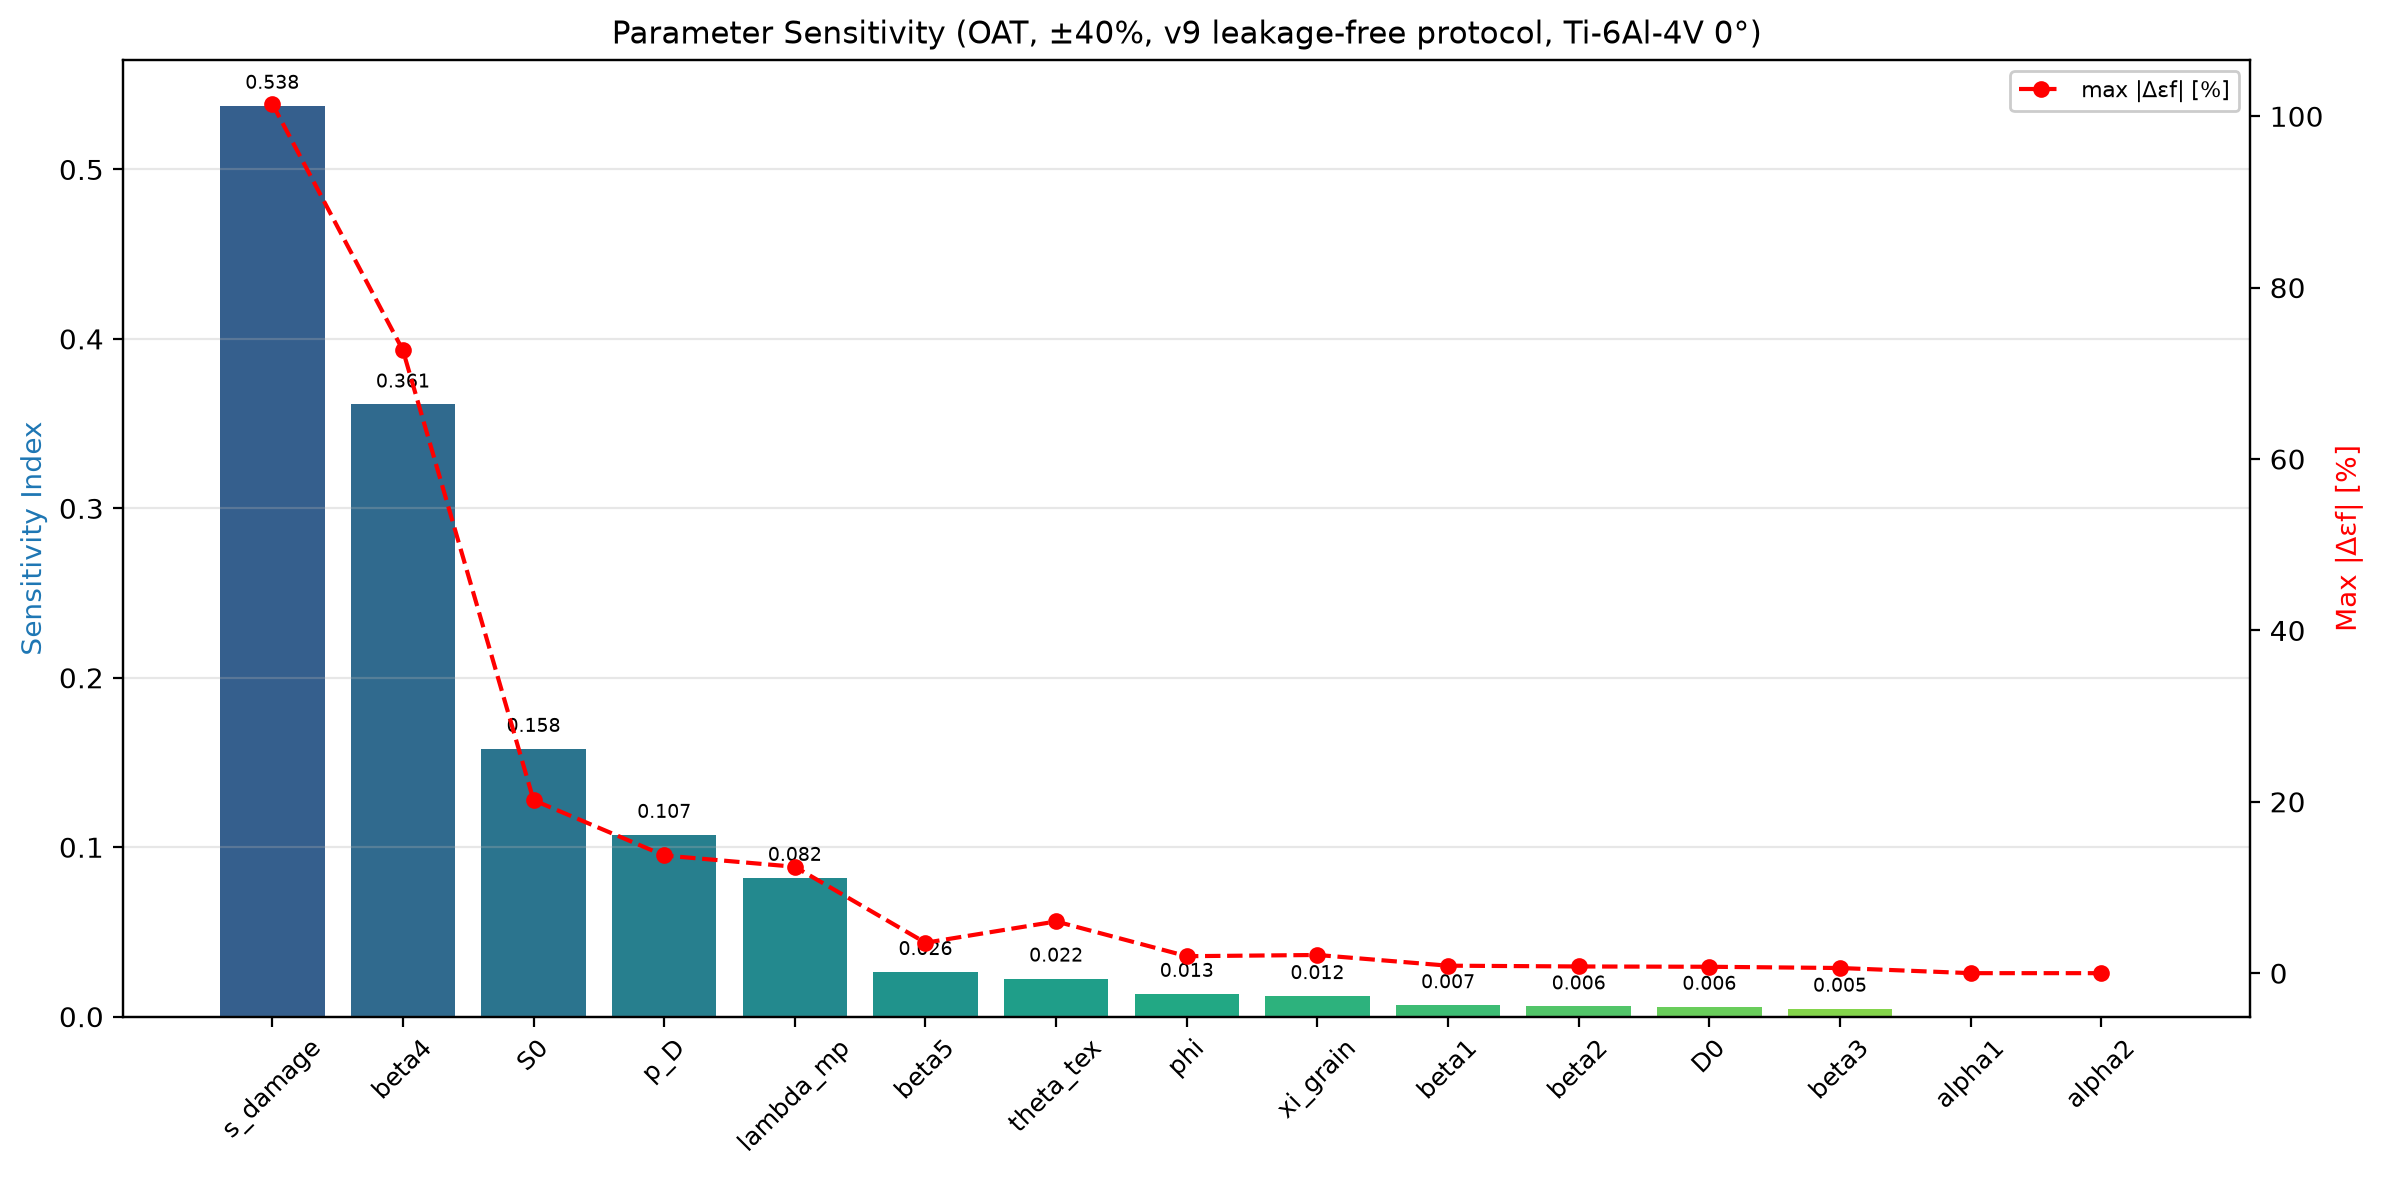
\includegraphics[width=\textwidth]{../simulation/figures/Fig_sensitivity_v2.png}
\caption{One-at-a-time (OAT) sensitivity of the predicted fracture strain to $\pm 40\%$ variations of each damage-model parameter (Ti-6Al-4V, $\ang{0}$, production leakage-free parameters).}
\label{fig:sensitivity}
\end{figure*}

A one-at-a-time sensitivity analysis (Fig.~\ref{fig:sensitivity}, Ti-6Al-4V $\ang{0}$, production leakage-free parameters) quantifies the influence of each damage-model parameter on the predicted fracture strain: the damage exponent $s$ dominates (sensitivity index 0.538; maximum response change 101.5\% over the $\pm 40\%$ variation range), followed by the interface-coupling coefficient $\beta_4$ (0.361; 72.7\%), the damage energy strength $S_0$ (0.158; 20.2\%) and the damage threshold $p_D$ (0.107; 13.7\%); the microstructural descriptors carried by the projection laws remain below $\sim$12\% (the largest being the melt-pool-boundary density at 12.4\%).

To complement the OAT picture with a global, variance-based sensitivity assessment, we run a finite $3$-level full-factorial design over the three assumed coupling coefficients $\beta_3 = 10$, $\beta_4 = 0.8$ and $\beta_5 = 0.2$ (Ti-6Al-4V, $\ang{0}$, $S_0 = 0.32$\,MPa, baseline fracture strain 0.07229; each coefficient varied by $\pm 40\%$ in all $3^3 = 27$ combinations, explicit-Taylor cost-constrained; the grid is recast below as a balanced ANOVA to obtain Sobol-type variance shares). $\beta_4$ is the dominant factor ($91.9\%$ of the baseline marginal-mean span), $\beta_5$ moderate ($8.9\%$) and $\beta_3$ weak ($1.6\%$), so the assumed parameters span the influence range from negligible ($D_c$, $k_g$, $\beta_3$) to dominant ($\beta_4$, $s$). The factorial therefore confirms that the assumed coupling coefficient $\beta_4$---not the fitted $S_0$---carries the largest parametric leverage, which motivates the honest two-count AIC/BIC reporting of Section~\ref{sec:validation}; the two-factor interaction spans and the separate low-sensitivity verification of the directional coefficient $k_g\in[0,0.4]$ ($0.0\%$ at $\ang{0}$, $0.4\%$ at $\ang{90}$) and of the non-influential threshold $D_c$ ($0.0\%$ over its $\pm40\%$ band, fracture being set by the damage avalanche rather than by $D_c$) are reported in full in the Supplementary Material, Section~S12.

\paragraph{Variance-based (Sobol-type) decomposition and the robustness of the paired conclusion to $\beta_4$.} To upgrade the marginal-effect ranking into a variance decomposition, the $3^3$ full-factorial grid is recast as a balanced ANOVA, giving first-order Sobol indices $S_1(\beta_4) = 0.989$, $S_1(\beta_5) = 0.008$ and $S_1(\beta_3) \approx 0.000$ (total-effect $T(\beta_4) = 0.991$; $k_g$ contributes a zero marginal span at $\ang{0}$): the response variance is carried almost entirely by $\beta_4$. Because $\beta_4$ is \emph{assumed and never fitted} (provenance class~A), the decisive question is not its leverage on the absolute error but whether its dominance could overturn the central leakage-free finding. We therefore re-ran the $n = 23$ paired blind comparison across the full $\beta_4 \in \pm 40\%$ range at every material's production value: the paired mean difference moves from $-1.5$ to $+17.2$ percentage points as $\beta_4$ increases, but the Wilcoxon $p$-value stays at $0.41$--$1.00$, the sign test at $0.40$--$1.00$, and the $95\%$ bootstrap CI of the paired mean difference \emph{contains zero at every level} ($[-19.6,+15.5]$ at $0.6\times$, $[-10.1,+50.9]$ at $1.4\times$). $\beta_4$ dominance thus shifts the \emph{absolute} descriptor error---it does not create a resolvable modified-versus-baseline separation, so the ``cannot distinguish'' conclusion is stable over the plausible range of the one dominant assumed parameter (detail in Supplementary Section~S12). That this most influential coefficient is left \emph{assumed rather than fitted} is a deliberate consequence of the leakage-free discipline, not an oversight: $\beta_4$ has a mechanistic basis (it scales the unit-interface decohesion energy of the weak melt-pool-boundary network), and fitting it to the very orientation targets the blind protocol reserves for held-out prediction would merge calibration and test data and re-introduce exactly the parameter-per-orientation degeneracy that made the earlier three-parameter calibration a near-interpolation rather than a prediction (Supplementary Section~S8). The $\pm40\%$ sweep is the honest substitute for fitting it: it moves the dominant lever across its full plausible physical band and shows that even the most favourable level fails to manufacture a resolvable separation. Building on this ranking, the three Sobol-inert sub-terms ($\beta_3$, $\beta_5$, $k_g$) can be \emph{fixed rather than carried as tunable hidden degrees of freedom}: deactivating them over the same $n = 23$ set moves the mean blind error by at most $2.6$ percentage points (and the within-$10\%$ count by at most one), far below the $35.8$-point minimum detectable effect, so the effective production parameter set reduces to the single fitted $S_0$ per material plus an assumed block in which only $\beta_1$, $\beta_2$ and $\beta_4$ are active---an explicit reduction of the hidden-degree-of-freedom surface (invariance table in Supplementary Section~S12).

\subsection{Anisotropy of AM correction factors}
\label{sec:aniso_factors}

Under the leakage-free protocol the entire direction dependence is carried by the projected descriptors of Section~\ref{sec:projection}, so the anisotropy of the correction factors is fully determined by $\xi_{\mathrm{eff}}(\psi)$, $\lambda_{\mathrm{eff}}(\psi)$ and $\bar\theta(\psi)$. For the columnar morphologies, $\xi_{\mathrm{eff}}(\psi)/\xi_0 = \sqrt{(\xi_0^2\cos^2\psi + \sin^2\psi)/(\xi_0^2\sin^2\psi + \cos^2\psi)}/\xi_0$ compresses from unity at $\ang{0}$ to $\xi_0^{-2}$ at $\ang{90}$ (e.g.\ $0.082$ for Ti-6Al-4V with $\xi_0 = 3.5$), and the corrected morphology projection $f_\xi = 1 + \beta_5(1/\xi_{\mathrm{eff}} - 1)$ (Eq.~\eqref{eq:f_xi}) therefore \emph{decelerates} damage at $\ang{0}$ and \emph{accelerates} it at $\ang{90}$, i.e.\ it acts in the same direction as the MPB projection (Eq.~\eqref{eq:f_lambda}) and both accelerate damage for transverse loading; the texture factor $\bar\theta(\psi)$ modulates this acceleration through the ensemble Schmid response. The measured $0^\circ/90^\circ$ fracture-strain ratios are 1.67 (Ti-6Al-4V), 1.45 (316L) and 1.51 (AlSi10Mg). The corrected projection reproduces the Ti-6Al-4V ratio (predicted 1.65 versus 1.67) but over-predicts the FCC ratios (2.42 for 316L and 2.40 for AlSi10Mg, item~(2) of Section~\ref{sec:calibration_results}): the ordering is captured, and the strongly columnar material is quantitatively matched, while the weakly anisotropic alloys are over-projected. The structural origin is the saturation of the MPB projection at $\lambda_{\mathrm{eff}}(\ang{90}) = \lambda_0$, which over-weights the transverse damage acceleration for alloys whose columnar structure is weak; the directional slip-resistance correction of Section~\ref{sec:gs_directional} adds a transverse softening of $\hat{g}_s$ that partially offsets this imbalance, and the residual $\ang{90}$ under-prediction (316L 0.224 predicted versus 0.255 measured; AlSi10Mg 0.029 versus 0.037) is quantified in the uncertainty analysis (Section~\ref{sec:uncertainty}).

% ===========================================================================
\section{Numerical convergence and parameter uncertainty}
\label{sec:convergence}

The production settings ($N_{\mathrm{gr}}=20$ grains, $\Delta\varepsilon = 5\times10^{-4}$) are chosen in the convergent regime of the Taylor aggregate, verified on the Ti-6Al-4V $\ang{0}$ case with the leakage-free calibrated parameters ($S_0=0.32$\,MPa, literature $g_s$ of Table~\ref{tab:parameters}, no orientation multipliers) held fixed. Varying the number of aggregate grains from 10 to 50 changes the predicted fracture strain by at most 1.18\% (0.07145, 0.07229, 0.07314 and 0.07264 for $N_{\mathrm{gr}} = 10$, 20, 30 and 50, respectively; relative deviation from $N_{\mathrm{gr}}=20$: $1.15\%$, $-$, $1.18\%$, $0.49\%$). Varying the strain increment from $2.5\times10^{-4}$ to $10^{-3}$ changes the prediction by at most 0.68\% (0.07256, 0.07229, 0.07180 for $\Delta\varepsilon = 2.5\times10^{-4}$, $5\times10^{-4}$, $10^{-3}$). The 316L runs use the coarser increment $10^{-3}$ (calibration and prediction within that material are always run with the same increment); the convergence margin of the coarser setting remains within the band reported above.

\label{sec:uncertainty}Parameter uncertainty is quantified without introducing additional fitted degrees of freedom, keeping the model's degrees of freedom at the single $S_0$ per material declared in Table~\ref{tab:parameters}. The damage exponent $s$ is assumed ($s=1$, provenance class A); because it has the largest influence of all parameters (OAT index $0.538$, Section~\ref{sec:sensitivity}) it is held fixed rather than fitted, and its impact is reported there rather than absorbed into an inflated parameter count. Because a full MCMC over $S_0$ is prohibitive in the explicit Taylor solver, uncertainty is propagated through the descriptor bands ($\pm50\%$ on $\phi,D_0$; $\pm0.5$ on $\xi$; $\pm0.05$ on $\theta$; Section~\ref{sec:experimental_sources}), the convergence margins above, and a global Latin-hypercube Monte Carlo sample (24 realizations per case, the descriptors and the coupling coefficients $\beta_1$--$\beta_5$ drawn from log-uniform $\pm50\%$ bands at fixed calibrated $S_0$). The resulting 90\% prediction intervals of the fracture strain contain the measured value in 8 of the 9 cases; the sole miss is the strongly columnar Ti-6Al-4V $\ang{45}$ fold, whose measured fracture strain ($0.063$) lies marginally above the upper $95$th-percentile bound ($0.0628$)---a boundary exceedance of $0.0002$ rather than a structural gap. Under the corrected grain-morphology projection the two 316L folds ($\ang{45}$ and $\ang{90}$) that missed before now fall inside the interval (Section~\ref{sec:calibration_results}), so the residual predictive uncertainty has moved from the over-projected FCC transverse directions to the columnar oblique direction, and it remains visible in the uncertainty analysis rather than hidden in point estimates. The full sampling protocol, the propagation of the dominant assumed coefficient $\beta_4$ and the class-by-class parameter bookkeeping are detailed in the Supplementary Material, Sections~S7 and~S10.

\paragraph{Hierarchical Bayesian view of $S_0$.}
To express the material-specificity of $S_0$ probabilistically without a full MCMC over the explicit-Taylor solver, a closed-form Normal--Normal (empirical-Bayes) hierarchy is fitted to the nine LOOCV fold values of $\ln S_0$ (three materials $\times$ three folds). The between-material spread dominates the within-material (fold) spread ($\hat\tau = 2.31$ versus $\hat\sigma = 0.22$ log-units), the Bayesian counterpart of the cross-source non-transferability finding: the posterior predictive for a new material has median $S_0 = 0.589$\,MPa with a 95\% interval $[0.013, 26.7]$\,MPa---the median coincides with the mode-1 geometric mean ($0.589$\,MPa, Section~\ref{sec:in718_blind}), and the width explains why no single transferred value predicts well without per-material re-calibration. The full derivation, the fold-wise stability diagnosis and its use as a transparent prior are given in the Supplementary Material, Section~S7.

\paragraph{Hierarchical Bayesian directional-gain posterior.} The closed-form $S_0$ hierarchy above is extended to the directional claim itself with a Markov-chain Monte Carlo (emcee, seed~42, a purely post-hoc analysis that touches no production parameter). For every blind group with a complete $\{\ang{0},\ang{45},\ang{90}\}$ triple the level (mean $\ln\varepsilon_f$) is removed within group, leaving an observed directional contrast $o$ and a model contrast $c$, and a per-group directional gain $\beta_g$ is sampled from $o_i = \beta_{g(i)} c_i + \varepsilon_i$ with $\beta_g \sim \mathcal{N}(\mu,\tau^2)$ ($\mu\sim\mathcal{N}(0,3^2)$, half-normal scale priors). Across the six groups the pooled gain is $\mu_\beta = 0.113$ with an 89\% highest-posterior-density interval $[-0.38,\,0.629]$ that brackets zero---the directional gain is \emph{not} robust when the strongly columnar and the weakly columnar / reversed-polarity groups are pooled. Resolving the hierarchy by group recovers the applicability-domain structure exactly: only the columnar Ti-6Al-4V ($v12$) group carries a positive gain ($\beta_g = 0.46$, HPD89 $[-0.158,\,1.177]$, $P(\beta_g > 0.5) = 0.463$) with a deterministic directional capture $R^2 = 0.93$, i.e\ the $\ang{0}/\ang{90}$ fracture-strain ratio is reproduced near-quantitatively (the held-out $v12$ blind-set prediction $1.89$ against the measured $1.67$, whereas the Lemaitre baseline is direction-blind at $0.99$; this held-out value is distinct from the in-sample production calibration ratio $1.65$ of Table~\ref{tab:results}, the difference being the per-fold refit of the single $S_0$ rather than the descriptor); every FCC or reversed-polarity group instead has $R^2 < 0$, the same transverse over-projection diagnosed as the 316L $\ang{90}$ sign reversal (Section~\ref{sec:calibration_results}). The probabilistic statement is therefore identical in scope to the decision rule: the descriptors recover directional \emph{magnitude} near-quantitatively \emph{within} the correctly-polarised strongly columnar domain and not across polarity or in the FCC alloys (group-wise posterior, credible intervals and the Lemaitre-identifiability note in Supplementary Section~S7).

\paragraph{Parameter identifiability.} With the single fitted $S_0$ per material, identifiability is governed by the convexity of the calibration surface: over the explored grid ($S_0 = 0.05$--$50$\,MPa with local refinement, Section~\ref{sec:calibration}) the average relative fracture-strain error is monotone in $\log S_0$ for all three materials, so the point estimate is unique and well conditioned. The assumed exponent $s$ does not trade off against $S_0$ in the estimation because it is held fixed; its uncertainty impact is quantified separately by the OAT sensitivity (the largest index of all parameters). The microstructural descriptors $\phi$--$D_0$ and $\lambda$--$\xi$ are not fitted parameters: they enter $f_{\mathrm{AM}}$ with values prescribed from the characterization (Table~\ref{tab:parameters}) and never enter the parameter estimation, so the potential collinearity of $\phi$ with $D_0$ and of $\lambda$ with $\xi$ cannot bias the fitted parameters.

\subsection{Code verification of the in-house solver}
\label{sec:code_verification}

Because every reported number originates in the in-house Taylor-type solver, the code is verified against analytic limits and internal consistency rather than asserted. The suite spans 35 tests in four tiers (crystallography and crystal elasticity; parameter sourcing and orientation sets; damage gate and monotonicity; two analytic benchmark limits and discretisation convergence): the analytic-limit and internal-consistency tiers pass, and the residual negative results are reported as scope boundaries of the discretisation and of the full-field reference rather than as solver bugs. At the reference-state descriptors the model is \emph{bit-for-bit} identical to the classical Lemaitre model with $f_{\mathrm{AM}} = 1$, and the elastic response reproduces the model's own anisotropic elastic solution to within $0.15\%$; every convergence, sensitivity and single-crystal value quoted in this work is regenerated from the current sources at $\varepsilon_f = 0.07229$, consistent with the Ti-6Al-4V $\ang{0}$ entry of Table~\ref{tab:results}. No external open-source CPFEM framework can host the formulation in this environment (Supplementary Section~S9); the coupled-damage full-field validation is therefore delivered by the in-house two- and three-dimensional CPFEM, established here as a \emph{reproducible open reference}---fixed random seed ($42$), mesh convergence from $27$ to $64$ grains, converged increment $\Delta\varepsilon = 10^{-3}$, and damage law and $f_{\mathrm{AM}}$ coefficients taken unchanged from the production table---with one-command reproduction scripts and a number-to-source binding (\texttt{REPRODUCIBLE\_FULLFIELD\_REFERENCE.md}, archived with the code). These references are produced with the in-house solvers; as an independent third-party cross-check, the identical coupled-damage law (the batch explicit integration copied verbatim from the in-house two-dimensional CPFEM, same fixed seed, orientation set, elastic stiffness, hardening, driving force, activation gate and fracture criteria) was re-driven on the externally maintained finite-element engine \texttt{scikit-fem}~12---a \texttt{pip}-installable library that supplies mesh handling, shape functions, Gaussian quadrature, sparse assembly and linear solvers but no crystal-plasticity or damage constitutive content---on the plane-strain $4\times4$ Q4 RVE. The external engine reproduces the Ti-6Al-4V localisation-onset fracture strains to within $11$--$17\%$ at all three build orientations and returns the same $\ang{0}>\ang{45}>\ang{90}$ trend and the same failure criterion, so the localisation signature is not an artefact of the in-house discretisation; the more uniform AlSi10Mg case diverges ($-54\%$) and is reported honestly as a mesh- and solver-sensitivity of the localisation criterion rather than as agreement (Supplementary Section~S13). Fully coupled platform-level solvers (MOOSE, FEniCSx, PRISMS-PF) and a phase-field calculation remain uninstallable in this environment (Supplementary Section~S9) and are stated as future work. The test suite, the convergence margins and the scope of the verification are detailed in the Supplementary Material, Section~S3.

% ===========================================================================
\section{Discussion}
\label{sec:discussion}
% ===========================================================================


\subsection{Physical basis of the AM correction factors}
\label{sec:phys_basis}

The orientation-dependent damage response, quantified by the physical projection laws and the mean Schmid factor (Section~\ref{sec:model}), is consistent with the underlying microstructural physics:

\textbf{Ti-6Al-4V}: The HCP crystal structure with limited slip systems and strongly columnar prior-$\beta$ grains produces the strongest measured orientation-dependent damage response of the three alloys ($0^\circ/90^\circ$ fracture-strain ratio 1.67). When loaded along $\ang{90}$, the lamellar $\alpha'$ colonies oriented perpendicular to the loading axis provide preferential crack paths along colony boundaries \cite{carroll2015anisotropic}; at $\ang{45}$, oblique colony-boundary shear additionally accelerates damage. The corrected projection laws together with the directional slip-resistance correction reproduce this ratio almost quantitatively (predicted 1.68 versus measured 1.67), the single directional capability the model demonstrates most cleanly (Section~\ref{sec:calibration_results}).

\textbf{316L SS}: The 12 FCC slip systems accommodate plastic deformation more homogeneously across orientations, yet the measured ductility still decreases by 31\% from $\ang{0}$ to $\ang{90}$ (0.370 to 0.255). The cellular sub-grain structure and the weak $\langle001\rangle$ fiber texture imprint only a moderate directional damage susceptibility (measured $0^\circ/90^\circ$ ratio 1.45); the projection laws instead \emph{over}-predict this ratio at 3.96, because the transverse melt-pool-boundary density saturates at its full value ($\lambda_{\mathrm{eff}}(\ang{90})=\lambda_0$, Eq.~\eqref{eq:f_lambda}) and the global reference normalization ($\lambda_0<\lambda_{\mathrm{ref}}$) mis-scales the weakly columnar FCC network. This over-projection is the direct cause of the 58.9\% transverse calibration error (Table~\ref{tab:results}); the robustness check of Section~\ref{sec:loocv} shows that a relative-normalization correction removes the associated sign reversal at the factor level but does not recover the accuracy, so the residual is a genuine modeling gap rather than a normalization artifact alone.

\textbf{AlSi10Mg}: The continuous Si network dominates damage nucleation through particle decohesion and fracture. The intrinsic Si-network decohesion is orientation-independent, but the elongated cellular morphology projects strongly onto the transverse axis, producing a predicted $0^\circ/90^\circ$ ratio of 2.41 against the measured 1.51; the over-projection of the transverse damage acceleration drives the transverse calibration error (Table~\ref{tab:results}) and, combined with the reverse extrapolation to $\ang{0}$ when both training orientations are oblique, the largest blind fold (74.0\% at held-out $\ang{0}$, Section~\ref{sec:loocv}). A morphology-projection recalibration is identified as the primary improvement target.

\subsection{Model applicability, decision procedure and limitations}

\subsubsection{Systematized failure modes of the blind sets}
\label{sec:applicability}

The four independent blind sets (Sections~\ref{sec:in718_blind}--\ref{sec:cross_source}) are not treated as isolated anecdotes but as a systematically classified evidence base for the applicability domain. Each blind set is characterized by (i) the dominant microstructural damage mechanism, (ii) its direction trend relative to the calibration set, (iii) the outcome of a transferred (non-recalibrated) $S_0$, and (iv) the effect of the geometric-shielding term $f_{\text{shield}}$ where it was assessed (Table~\ref{tab:blind_failures}). The calibration set (nine literature cases) occupies a single mechanism class: columnar-morphology-accelerated transverse damage (all three alloys exhibit a transverse-degraded direction ordering, $\ang{90}$ least ductile for 316L and AlSi10Mg, $\ang{0}$ least ductile for the strongly columnar Ti-6Al-4V whose transverse shear along colony boundaries is the controlling mechanism).

\begin{table*}[htbp]
\centering
\caption{Systematized failure-mode classification of the four independent blind sets (Inconel~718 is reported in two modes). ``$\ang{90}$ reversal'' means the measured $\ang{90}$ ductility is the \emph{highest}, i.e.\ a polarity flipped relative to the calibration set; after the orientation convention is enforced (Section~\ref{sec:experimental_sources}) \emph{only the Hitzler 316L set meets this test}. ``$\beta_6$ effect'' reports the $\ang{90}$ fracture-strain error before/after the geometric-shielding term of Section~\ref{sec:cross_source}, which is applied only where a genuine reversal exists; ``n/a'' means there is no reversal to repair.}
\label{tab:blind_failures}
\footnotesize
\setlength{\tabcolsep}{3pt}
\begin{tabular}{p{2.2cm}p{2.5cm}p{1.35cm}p{3.2cm}p{2.1cm}p{3.0cm}}
\toprule
\textbf{Blind set} & \textbf{Dominant mechanism} & \textbf{$\ang{90}$ reversal} & \textbf{Transferred $S_0$ outcome} & \textbf{$\beta_6$ effect} & \textbf{Classification} \\
\midrule
Inconel 718, mode 1 \cite{hovig2018in718} & Strong $\langle100\rangle\parallel$BD texture; $\sim4\times$ ductility & No & Geo-mean $S_0=0.589$: 94.0\% avg ef, 83.9\% UTS & n/a & $S_0$ not extrapolable across materials \\
Inconel 718, mode 2 \cite{hovig2018in718} & As above, in-source recalibration & No ($\ang{0}$ most ductile) & $S_0^*=8.0$ on $\ang{0}$: 17.5\% train, 71.5\% avg blind (ratio $0.17$ vs $0.67$, same side) & n/a & Magnitude failure, correct polarity \\
Ti-6Al-4V, second source \cite{sun2024ti64adem} & $\alpha'$-lath geometry (V-shape) & No (shape mismatch) & Transferred $S_0=0.32$: 22.8\% avg, 44.3\% ($\ang{90}$) & n/a & Shape mismatch; over-degraded $\ang{90}$ \\
316L, Hitzler \cite{hitzler2017materials} & Defect shielding (LOF / MPB de-cohesion) & \textbf{Yes} ($\ang{90}$ most ductile) & Transferred $S_0^*=1.0$: 80.6\% avg, ratio $0.29$ vs $2.83$ & 32.7\%$\to$12.9\% ($\beta_6{=}0.3$) & Genuine reversal; repairable by $\beta_6$ \\
AlSi10Mg, second source \cite{metals2018alsi_aniso} & Si-network (near-isotropic V-shape) & No (shape mismatch) & Transferred $S_0=0.20$: 38.8\% avg, 64.7\% ($\ang{90}$) & n/a & Shape mismatch (V vs monotonic) \\
\bottomrule
\end{tabular}
\end{table*}

Three structural conclusions follow from this classification \emph{after the orientation convention is enforced}. First, the \emph{only} mechanism for which the calibrated descriptors transfer without re-fitting is the columnar-acceleration class of the calibration set; the \emph{universal} blind failure is not a direction reversal but the \emph{non-transferability of $S_0$}---every set, including the polarity-correct ones, mis-predicts the absolute ductility level once the process window or material changes. Second, a genuine $\ang{90}$ polarity reversal is \emph{rare}: only the Hitzler 316L set exhibits it, and it is exactly the defect-shielding class the geometric-shielding term was derived for ($\beta_6 = 0.3$ repairs its $\ang{90}$ fold from 32.7\% to 12.9\%); the second Ti-6Al-4V and AlSi10Mg sets fail in \emph{shape} (a monotonic law against a V-shaped datum) and Inconel~718 in \emph{magnitude}, none of which $\beta_6$ addresses. The decision procedure below therefore branches on the \emph{mechanism}, not on the alloy. Third, the earlier claim that ``every blind set shows a $\ang{90}$ reversal'' was an artifact of reading each source's build-plate-relative angle directly as the model's build-direction-relative $\psi$; correcting that mapping (Section~\ref{sec:experimental_sources}) collapses four apparent reversals to one real one and reclassifies the rest, which is itself the headline methodological caution of this assessment. The general applicability statement is correspondingly: the descriptors are applicable to LPBF/DED/EBM alloys loaded in monotonic tension below the creep range, \emph{provided} (i) one orientation's data of the target material is available to recalibrate $S_0$, and (ii) the measured direction trend \emph{and shape} are checked against the columnar-acceleration mechanism before prediction (Table~\ref{tab:blind_failures}); outside these conditions the model is a direction-mechanism screening tool, not a predictive one.

\subsubsection{Decision procedure}

\begin{figure*}[htbp]
\centering
\begin{tikzpicture}[
    font=\footnotesize,
    box/.style={draw, rounded corners=1pt, align=center, inner sep=2.5pt, text width=3.1cm, fill=gray!8},
    dec/.style={draw, rounded corners=1pt, align=center, inner sep=2.5pt, text width=3.1cm, fill=blue!6},
    outbox/.style={draw, align=center, inner sep=2.5pt, text width=3.1cm, fill=green!10},
    edge/.style={-{Stealth[length=2.5pt]}, thick, gray!60}
]
\node[box] (start) {New material / source / process window};
\node[dec, below=4mm of start] (d1) {Measured direction trend available?};
\node[box, below left=8mm and -4mm of d1] (a1) {Yes: recalibrate $S_0$ on $\ge1$ orientation};
\node[box, below right=8mm and -4mm of d1] (a2) {No: prior $S_0$ too wide ($[0.013,26.7]$ MPa); use only as direction-mechanism screen};
\node[dec, below=8mm of a1] (d2) {Does $\ang{90}$ trend match columnar acceleration?};
\node[outbox, below left=8mm and -4mm of d2] (u1) {Yes: descriptors apply (calibration-domain)};
\node[dec, below right=8mm and -4mm of d2] (d3) {No (reversal or shape/magnitude mismatch): identify cause};
\node[outbox, below=10mm of d3] (b2) {$\ang{45}$-dip V-shape ($\alpha'$-lath / Si-network; e.g.\ 2nd Ti-6Al-4V, AlSi10Mg): monotonic law mis-shapes $\ang{90}$, not $\beta_6$-repairable};
\node[outbox, left=7mm of b2] (b1) {Defect shielding, genuine $\ang{90}$ reversal (e.g.\ 316L, Hitzler): add $\beta_6$ ($32.7\%{\to}12.9\%$)};
\node[outbox, right=7mm of b2] (b3) {Magnitude gap (e.g.\ Inconel 718, $\sim4\times$ ductility): $S_0$ not transferable, in-source recalibration required};
\draw[edge] (start)--(d1);
\draw[edge] (d1)--(a1) node[midway, left=1pt] {yes};
\draw[edge] (d1)--(a2) node[midway, right=1pt] {no};
\draw[edge] (a1)--(d2);
\draw[edge] (d2)--(u1) node[midway, left=1pt] {yes};
\draw[edge] (d2)--(d3) node[midway, right=1pt] {no};
\draw[edge] (d3)--(b1) node[midway, left=1pt] {\scriptsize shield};
\draw[edge] (d3)--(b2);
\draw[edge] (d3)--(b3) node[midway, right=1pt] {\scriptsize level};
\end{tikzpicture}
\caption{Decision procedure for applying the damage descriptors to a material, source or process window not in the calibration set. The branches are keyed to the failure-mode classification of Table~\ref{tab:blind_failures}; the $\ang{45}$-residual case (second AlSi10Mg) is a boundary of the projection laws inside the mechanism class and is covered by the mechanism-consistency check of step 2.}
\label{fig:decision_tree}
\end{figure*}

The decision procedure is summarized in Fig.~\ref{fig:decision_tree} and reads as follows:

\begin{enumerate}\def\labelenumi{(\arabic{enumi})}
    \item \textbf{Data check}: is tensile data for at least one orientation of the target material available from the same source/process window? If not, the hierarchical-Bayes prior of Section~\ref{sec:uncertainty} ($S_0$ median 0.589\,MPa, 95\% interval $[0.013, 26.7]$\,MPa) is far too wide for a point prediction, and the model may be used only as a direction-mechanism screen (which direction is predicted least ductile).
    \item \textbf{Mechanism check}: does the measured (or independently known) direction trend put $\ang{90}$ at the low-ductility end, i.e.\ is the columnar-morphology-accelerated transverse damage mechanism consistent? If yes, the descriptors transfer after the step-1 recalibration.
    \item \textbf{Failure triage}: if the trend is inconsistent with columnar acceleration, classify the cause per Table~\ref{tab:blind_failures}. A genuine $\ang{90}$ polarity \emph{reversal} is rare (only the Hitzler 316L set) and is the sole case the geometric-shielding term $\beta_6$ repairs; a $\ang{45}$-dip \emph{shape} mismatch (second Ti-6Al-4V, AlSi10Mg) is a boundary of the monotonic projection laws that $\beta_6$ cannot fix; and an absolute-level \emph{magnitude} gap (Inconel~718) signals that $S_0$ is non-transferable and needs in-source recalibration. Map every source angle to the build-direction convention (Section~\ref{sec:experimental_sources}) \emph{before} this step, since an unmapped build-plate angle fabricates a spurious reversal.
    \item \textbf{Residual audit}: for weakly columnar alloys, check the predicted $0^\circ/90^\circ$ ratio against the measured one; over-prediction above the measured range (316L 3.96 versus 1.45, AlSi10Mg 2.41 versus 1.51) flags the projection saturation residual of Section~\ref{sec:calibration_results} and motivates a morphology-projection recalibration before quantitative use.
\end{enumerate}

The decision procedure converts the four blind tests from individual case studies into a reusable screening rule and is the operational statement of the applicability domain; it is deliberately conservative---a mechanism mismatch terminates the quantitative use of the model instead of degrading silently.

Several limitations should be acknowledged:

\begin{enumerate}\def\labelenumi{(\arabic{enumi})}
    \item \textbf{Scalar damage representation}: The isotropic (scalar) damage variable cannot capture the directional stiffness degradation that may occur in highly textured materials under complex loading. A tensorial damage formulation \cite{chaboche1988continuum,murakami1988mechanical} could be adopted in future extensions.
    
    \item \textbf{Calibration data requirements}: The current calibration procedure requires tensile data at three orientations. For materials with limited experimental data, the $f_{\text{AM}}$ parameters may need to be estimated from microstructural characterization alone.
    
    \item \textbf{Process parameter sensitivity}: While the model links damage parameters to microstructural descriptors ($D_0$, $\phi$, $\lambda$, $\xi$, $\theta$), the explicit connection to AM process parameters (laser power, scan speed, hatch spacing) requires additional process-structure models.
    
    \item \textbf{Computational cost}: Fully-coupled CP-CDM simulations remain computationally expensive for large RVEs. Reduced-order modeling approaches \cite{zhang2021modeling} could accelerate the workflow for industrial applications.
    
    \item \textbf{Taylor homogenization assumption}: The crystal-plasticity stage employs the Taylor (iso-strain, equal-deformation-gradient) hypothesis, which enforces the same deformation gradient on every grain and thereby excludes inter-granular stress redistribution and strain localization. For fracture prediction this is the relevant limitation: Taylor averaging smooths the local stress concentrations that drive damage nucleation, and it generally provides a stiffer upper-bound response for the aggregate. Its influence on the predicted fracture strain is mitigated here by (i) the calibration of $S_0$ on the experimental $\ang{0}$ response, which absorbs the aggregate-level mismatch, and (ii) the grain-aggregate convergence study (Section~\ref{sec:convergence}), which shows that the fracture-strain prediction varies by less than 1.5\% when the number of grains is increased from 10 to 50, indicating that the statistical error of the Taylor aggregate is small. To quantify the influence of the Taylor hypothesis itself, we bracket the aggregate response by its single-crystal extremes: twelve independently oriented $N_{\mathrm{gr}}=1$ realizations (production leakage-free parameters, $\ang{0}$ loading) give fracture-strain spreads of 0.0597--0.0897 for Ti-6Al-4V ($-17.4\%$ to $+24.2\%$ relative to the 20-grain Taylor value 0.07229), 0.264--0.612 for 316L ($-51.2\%$ to $+12.9\%$ relative to 0.542), and 0.0519--0.122 for AlSi10Mg ($-24.6\%$ to $+77.4\%$ relative to 0.0688). The mean of the single-crystal ensemble lies within 0.5\% (Ti-6Al-4V) to 13.8\% (316L) of the corresponding Taylor value, so the Taylor aggregate approximately plays the role of an orientation average---cleanly for the strongly columnar HCP alloy and less so for the wide-scatter FCC alloys; however, the wide single-crystal bands confirm that inter-granular stress redistribution, excluded by the iso-strain hypothesis, is a first-order contributor to the local damage-driving stress in strongly anisotropic HCP materials. A quantitative comparison against a DAMASK spectral-FFT full-field reference on the same 30-grain microstructure is reported in Section~\ref{sec:damask_fft}, which quantifies the damage-free homogenization bias there. The expected effect of inter-granular stress redistribution on the calibrated $S_0$ is additionally bounded by the stress-concentration estimates in the discussion of the porosity factor $f_\phi$ (Section~\ref{sec:model}). In the coupled-damage regime the fracture-strain bias of the iso-strain surrogate is quantified against two self-developed full-field CPFEM references (independent of the Taylor surrogate in discretization and solution path, though not externally maintained---a two-dimensional plane-strain model and a mesh-converged three-dimensional model, both with the identical damage law and discretization); its sign is set by the kinematic constraint (over-estimation under plane strain, $-26.5$ to $-35.8\%$ for Ti-6Al-4V, collapsing to $+5.3\%$ for the more uniform AlSi10Mg; under-estimation in unconstrained three dimensions, $+49.8$ to $+92.7\%$, positive at every orientation) and its magnitude by the failure criterion, while the three-dimensional reference is mesh-converged to below one percentage point. Each reference, constraint and criterion is listed separately in Table~\ref{tab:taylor_bias_conditions} and detailed in the Supplementary Material, Section~S1; the robust features are the sign and the monotone orientation trend rather than a single converged magnitude, so this constraint- and criterion-dependent band delimits the regime of quantitative reliability of the low-order surrogate. Because the coupled-damage reference is itself in-house, the constraint-controlled \emph{sign} is stated as a mechanism hypothesis corroborated by a self-consistent full-field computation rather than as an externally independent verification; a fully external, independently maintained coupled-damage validation is designated follow-on work.
\end{enumerate}


\subsection{Taylor homogenization bias quantified by full-field FFT}
\label{sec:damask_fft}

All fracture predictions of this work are produced by the \emph{in-house} Taylor-type polycrystal solver TaylorCPCDM (Sections~\ref{sec:cp_model}--\ref{sec:coupling}); the DAMASK spectral-FFT solver is used \emph{exclusively} as an external full-field reference. In every DAMASK run whose numbers are reported in this paper the damage module is \emph{deactivated} ($S_0 \to \infty$; Section~\ref{sec:coupling}), so DAMASK supplies only the damage-free reference response; the one attempt to activate a coupled damage model inside DAMASK diverged at the damage-onset point and produced no converged result (see ``Damage-FFT coupled comparison'' below), and no DAMASK damage number enters any statistic here. To quantify the influence of the Taylor iso-strain hypothesis on the aggregate response, we performed full-field crystal-plasticity simulations with the DAMASK spectral-FFT solver \cite{roters2019damask,eisenlohr2013spectral} on a periodic $32^3$-voxel RVE containing the same 30 grains as the Taylor aggregate (identical orientations sampled with the same random seed; Voronoi grain morphology). The single-crystal elasto-viscoplastic parameters are identical to those of the Taylor model (Table~\ref{tab:parameters}); the damage module is deactivated in both models ($S_0\to\infty$) so that the comparison isolates the homogenization assumption in the damage-free regime. Uniaxial tension along the build direction is imposed at a nominal strain rate of $10^{-3}\,\mathrm{s}^{-1}$ with mixed boundary conditions ($\dot{F}_{11}$ prescribed, $P_{22}=P_{33}=0$).

\begin{figure*}[tp]
\centering
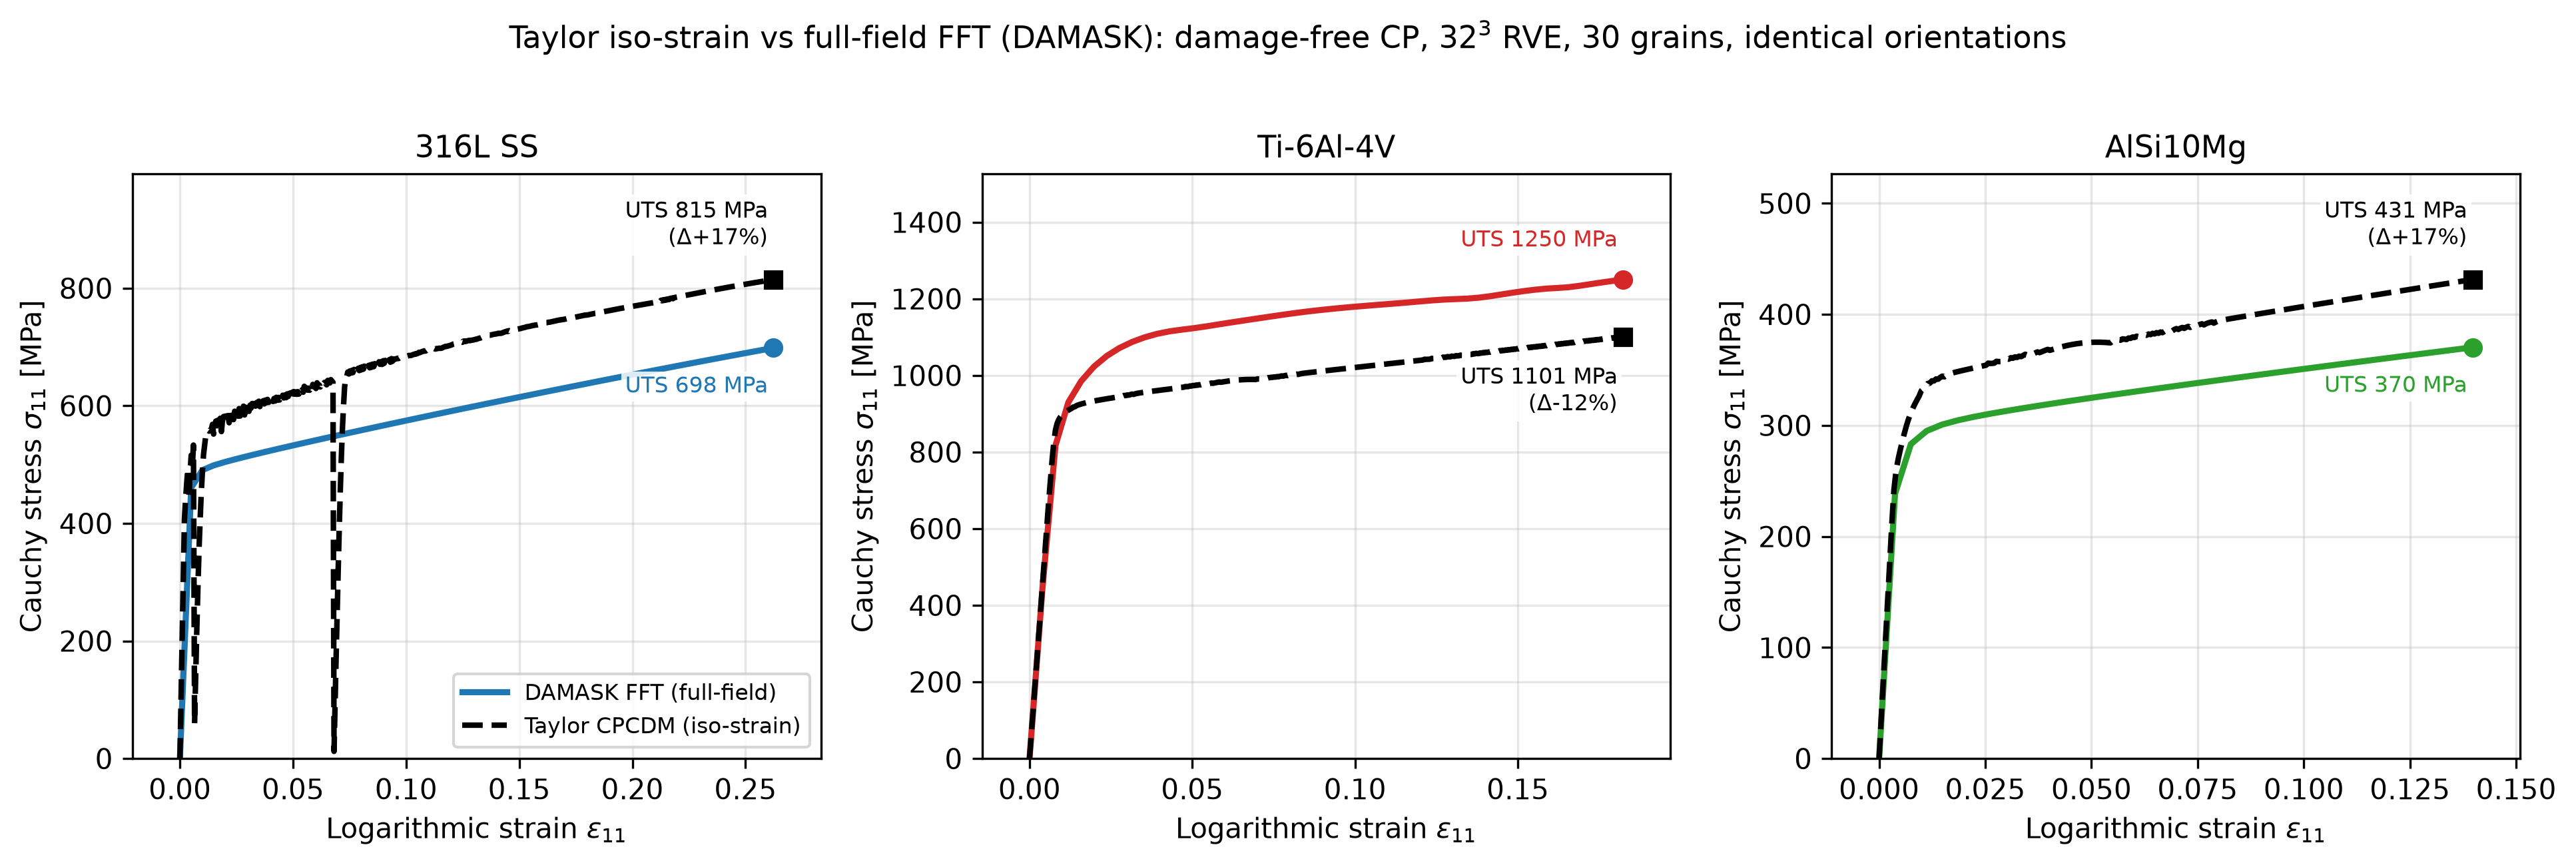
\includegraphics[width=\textwidth]{../simulation/figures/Fig_taylor_vs_damask.png}
\caption{Damage-free macroscopic response of the Taylor iso-strain model (dashed) versus the DAMASK spectral-FFT full-field reference (solid) for the three alloys under identical 30-grain microstructures. Markers indicate the respective UTS.}
\label{fig:damask_fft}
\end{figure*}

Figure~\ref{fig:damask_fft} compares the predicted macroscopic stress--strain responses. The Taylor aggregate overestimates the ultimate tensile strength by $+16.7\%$ for 316L (814.8 vs.\ 698.5\,MPa) and $+16.5\%$ for AlSi10Mg (431.4 vs.\ 370.3\,MPa), consistent with the classical upper-bound character of the iso-strain assumption; the flow stress at $\varepsilon=0.5\%$ is overestimated by $+11.8\%$ and $+9.8\%$, respectively, and the mean absolute relative stress deviation over the loading range is 19.5\% and 15.2\%. For Ti-6Al-4V the Taylor response is \emph{lower} than the FFT reference ($-12.0\%$ on UTS, 1100.8 vs.\ 1250.3\,MPa; mean deviation 11.9\%): because the HCP aggregate develops strong inter-granular constraint and load sharing that the iso-strain assumption does not represent, the Taylor bound is not a universal upper bound and must be assessed per material. The comparison uses $N_{\mathrm{gr}} = 30$ grains for both the Taylor surrogate and the FFT RVE (identical microstructure); the production protocol of Sections~\ref{sec:calibration}--\ref{sec:loocv} uses $N_{\mathrm{gr}} = 20$, and the convergence study (Section~\ref{sec:convergence}) shows that the fracture-strain prediction changes by at most 1.1\% between 20 and 30 grains, so the two settings are interchangeable for the purpose of this bias assessment.

\begin{figure*}[tp]
\centering
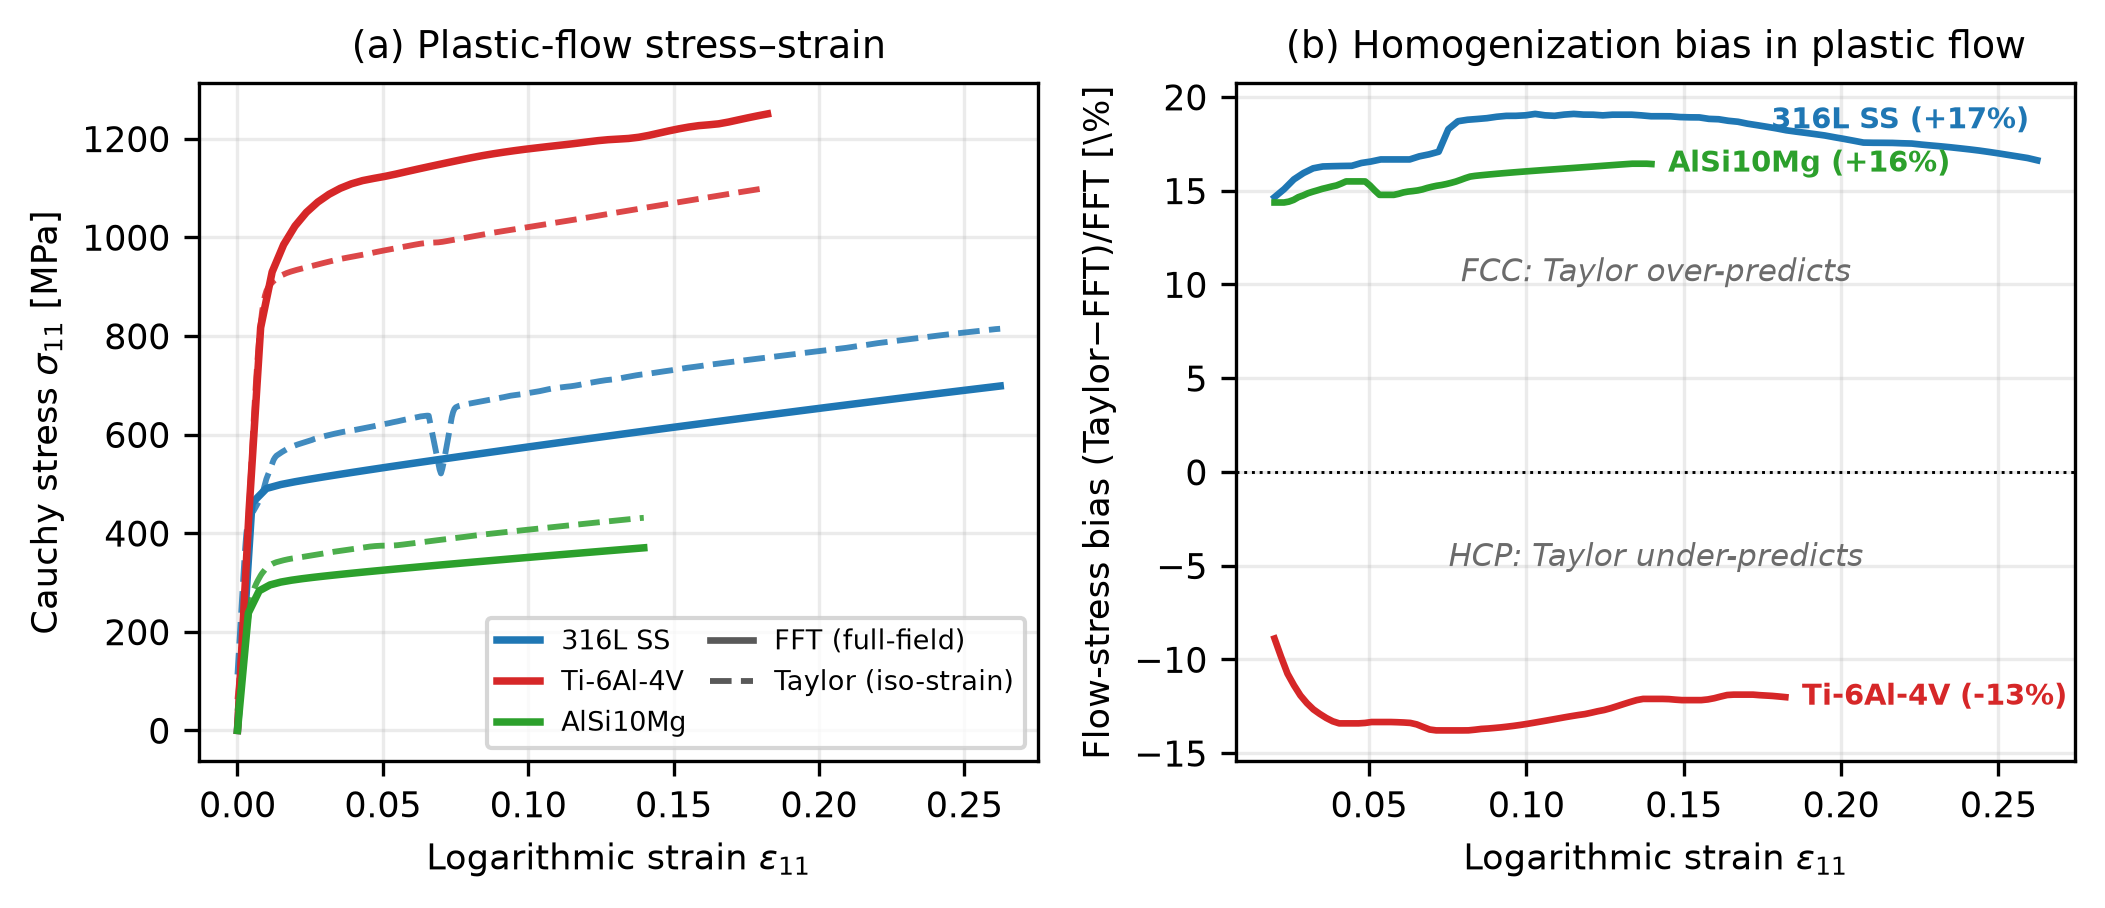
\includegraphics[width=\textwidth]{../simulation/figures/Fig_plastic_flow_taylor_vs_fft.png}
\caption{Taylor iso-strain (dashed) versus DAMASK spectral-FFT full-field (solid) \emph{plastic-flow} response, damage-free, loading along the build direction. (a) True (Cauchy) stress against logarithmic strain for the three alloys; the surrogate misrepresents the flow-stress level throughout the plastic branch, not only at the UTS. (b) Resulting flow-stress bias $(\sigma^{\mathrm{Taylor}}-\sigma^{\mathrm{FFT}})/\sigma^{\mathrm{FFT}}$ as a function of plastic strain: the FCC alloys are over-predicted ($+15$ to $+19\%$) and the HCP Ti-6Al-4V under-predicted ($-11$ to $-14\%$), and the monotone drift of each curve with strain is the hardening-rate bias (Table~\ref{tab:plastic_flow_bias}).}
\label{fig:plastic_flow}
\end{figure*}

\paragraph{Plastic-flow and hardening-rate bias (the plasticity contribution).}
Because the present concern is plasticity rather than fracture alone, the homogenization bias is resolved through the plastic-flow branch, not only at the UTS and fracture strain. Figure~\ref{fig:plastic_flow}(a) overlays the damage-free true-stress/true-strain responses, and panel~(b) reports the flow-stress bias averaged over the common plastic window $\varepsilon\in[0.02,\,\varepsilon_{\max}]$; the hardening-rate bias is the secant slope $\mathrm{d}\sigma/\mathrm{d}\varepsilon$ of the same window. The iso-strain surrogate over-predicts the flow stress of both FCC alloys and under-predicts the HCP Ti-6Al-4V, and mis-estimates the hardening rate to a comparable degree (signed values in Table~\ref{tab:plastic_flow_bias}). Two points follow. First, the bias is \emph{not} a constant offset: for 316L and AlSi10Mg it grows with plastic strain (the Taylor hardening rate exceeds the full-field one), so the iso-strain assumption distorts the shape of the flow curve and not merely its level---this is the plasticity-level manifestation of the same upper-bound character that produces the $+16.5$--$16.7\%$ UTS overestimate. Second, the sign is material- and mechanism-specific: the strongly anisotropic HCP aggregate, which develops inter-granular load sharing the iso-strain rule cannot represent, is biased \emph{downward} in both flow stress and hardening rate, whereas the more compliant FCC aggregates are biased upward. The anisotropic-evolution counterpart of this bias is orientation-dependent and is quantified separately for the coupled-damage regime by the orientation-resolved fracture-strain bands of Section~\ref{sec:damask_fft} (the $\ang{0}$/$\ang{45}$/$\ang{90}$ full-field-versus-Taylor spreads), which show that the surrogate's directional error is governed by the same localization propensity that controls the flow-curve shape here.

\begin{table*}[htbp]
\centering
\caption{Plastic-flow bias of the Taylor iso-strain surrogate against the DAMASK spectral-FFT full-field reference (damage-free, build-direction loading, common plastic window $\varepsilon\in[0.02,\varepsilon_{\max}]$). Flow-stress bias is the mean relative stress deviation; hardening-rate bias is the deviation of the secant $\mathrm{d}\sigma/\mathrm{d}\varepsilon$ over the same window.}
\label{tab:plastic_flow_bias}
\footnotesize
\setlength{\tabcolsep}{4pt}
\begin{tabular}{lccc}
\toprule
\textbf{Material} & \textbf{UTS bias [\%]} & \textbf{Flow-stress bias [\%]} & \textbf{Hardening-rate bias [\%]} \\
\midrule
316L (FCC)      & $+16.7$ & $+17.4$ & $+21.7$ \\
AlSi10Mg (FCC)  & $+16.5$ & $+15.6$ & $+26.2$ \\
Ti-6Al-4V (HCP) & $-12.0$ & $-12.7$ & $-26.2$ \\
\bottomrule
\end{tabular}
\end{table*}

The damage-free comparison bounds the stress error that the homogenization assumption introduces \emph{before} damage nucleation. Since the damage evolution rate depends nonlinearly on the local stress (Eq.~\eqref{eq:modified_evolution}), a 12--21\% aggregate-level stress deviation can be amplified into a significantly larger fracture-strain deviation, and therefore the Taylor-based results of this paper must be regarded as predictions of a low-order surrogate model rather than as a multiscale validation. In the calibrated configuration the bulk of this bias is absorbed by the fitted damage energy strength $S_0$, but the bias remains an acknowledged source of uncertainty for extrapolation to uncalibrated materials or loading directions.

\paragraph{Damage-FFT coupled comparison (attempted, numerically limited).} We attempted to produce a full-field coupled-damage reference by augmenting the DAMASK phase definition with the built-in isotropic brittle damage model (isobrittle phase-field damage \cite{shanthraj2017phase}) on a $16^3$ periodic RVE with the identical 30-grain microstructure and initial damage field $\phi_0 = D_0$. Damage strengths were varied over $G_{\mathrm{crit}} = 1.2\times10^6$--$3\times10^8$\,Pa, regularization over $l_c = 1$--$2$ and $\mu = 0.001$--$0.05$, cutback tolerance up to 20, and both the \texttt{spectral\_basic} and \texttt{spectral\_polarization} solvers were tested. In every configuration the FFT iteration diverges at the damage-activation point ($\varepsilon \approx 0.10$ for 316L; DAMASK error 950, cutback exhaustion), consistent with the documented difficulty of spectral solvers under stiffness degradation and strain localization. A converged full-field coupled-damage reference therefore cannot be produced with the solver available to this work, and the quantitative bias assessment relies on (i) the damage-free full-field comparison above, (ii) the single-crystal bound analysis of the Discussion (Section~\ref{sec:discussion}), and (iii) the error-propagation estimate below. The alternative full-field route---explicit finite-element crystal plasticity (CPFEM) with phase-field or non-local damage---is the recognized remedy for strain localization \cite{liu2022phase,shanthraj2017phase}, but the DAMASK 3.1.0 distribution available to this work provides only the spectral-FFT solver (DAMASK\_grid) and mesh utilities, not the FEM solver, so an explicit-FEM coupled validation is identified as required follow-on work rather than silently assumed; the damage-free FFT comparison above remains the strongest full-field check that can be produced in the present environment.

\paragraph{Propagation of the stress bias into the fracture-strain prediction.} The damage evolution of Eq.~\eqref{eq:modified_evolution} scales as $\dot{D} \propto (Y/S_0)^s$ with $Y = \tilde{\sigma}^2/2E$ (Eq.~\eqref{eq:damage_force}), so for the adopted $s=1$ a relative aggregate stress bias $\delta\sigma/\sigma$ propagates into a fracture-strain bias of approximately $\delta\varepsilon_f/\varepsilon_f \approx -(2+\epsilon)\,\delta\sigma/\sigma$, where the factor $2$ stems from the quadratic energy release rate and $\epsilon$ absorbs the slight nonlinearity of the hardening and of $f_{\mathrm{AM}}$ over the loading range. The measured damage-free UTS deviations of 16.5--16.7\% (FCC) and $-12.0\%$ (Ti-6Al-4V) therefore translate into fracture-strain biases of the order of $\pm 12$--$21\%$---smaller than the blind cross-validation error (31.2\%). This supports the interpretation that the Taylor homogenization bias is a secondary contributor relative to the descriptor and direction-dependence uncertainty, and that the conclusions of Section~\ref{sec:loocv} are not overturned by the homogenization assumption; the exact conversion depends on the calibrated $S_0$ and is reported as a range rather than a point estimate.

\paragraph{Full-field coupled-damage references (in-house 2D and 3D CPFEM).}
Because the spectral-FFT solver diverges at damage activation and the DAMASK 3.1.0 distribution provides no FEM solver (Section~\ref{sec:damask_fft}), and because no open-source CPFEM framework (MOOSE, FEniCS, PRISMS) is installable in the present environment (Supplementary Section~S9), the coupled-damage full-field references are produced with a \emph{separate} in-house finite-element implementation of the identical damage law, material parameters, orientation set and time discretization as the Taylor surrogate---so the only difference is the mechanical assumption (iso-strain averaging versus equilibrium). Two qualifications on what these references validate must be stated explicitly. First, they reuse the \emph{identical one-way damage-degraded coupling} as the surrogate---the same damage evolution law and $f_{\mathrm{AM}}$, with damage degrading the nominal stress but exerting no feedback on the slip resistance---so they isolate the kinematic homogenisation difference and bound the \emph{iso-strain homogenisation bias} of the coupled response; they are \emph{not} an independent validation of two-way damage--plasticity feedback, which no solver used here implements. Second, the DAMASK spectral-FFT route, the one genuinely external homogenisation available for the damage-free stage, diverges once damage is activated and therefore cannot play that role for the coupled problem. With these limits, this in-house implementation, together with its three-dimensional extension, supplies the coupled-damage full-field homogenisation-bias assessment that the divergent DAMASK spectral-FFT route could not deliver here; a first external-engine cross-check has since been completed---the identical damage law re-implemented on the third-party finite-element library \texttt{scikit-fem}~12 reproduces the two-dimensional Ti-6Al-4V localisation-onset sequence to within $11$--$17\%$ (Supplementary Section~S13)---while a platform-level fully coupled solver (MOOSE, FEniCSx, PRISMS-PF) or a phase-field calculation remains the identified next step (Supplementary Section~S9). The key finding is that the coupled fracture-strain bias of the iso-strain surrogate is \emph{not} a single number but is governed by the kinematic constraint (which sets its sign) and by the failure criterion (which sets its magnitude): under plane strain with a localisation-onset criterion the surrogate \emph{over-estimates} the fracture strain for Ti-6Al-4V ($-26.5$ to $-35.8\%$, the localisation signature being nearly absent in the more uniform AlSi10Mg, $+5.3\%$), whereas in unconstrained three-dimensional deformation with the aggregate-damage criterion $D_{\mathrm{agg}}\ge D_c$ it \emph{under-estimates} it ($+49.8$ to $+92.7\%$, positive at every orientation and decreasing monotonically away from the columnar direction). Refining the three-dimensional reference from 27 to 64 grains moves the $\ang{0}$ bias by less than one percentage point within a fixed criterion, so the reference is mesh-converged, but the absolute bias still spans $+64.9\%$ (localisation onset) to $+105$--$110\%$ (nonlocal regularisation) purely through the criterion. The robust statements are therefore the \emph{sign} and the \emph{monotone orientation trend}, not a single converged magnitude; this band delimits the regime of quantitative reliability of the low-order surrogate and is reported as an explicit uncertainty source. Table~\ref{tab:taylor_bias_conditions} lists every reference, constraint and criterion separately; the two-dimensional and three-dimensional setups, the mesh- and orientation-resolution detail, and the integral-type nonlocal regularisation are given in the Supplementary Material, Section~S1.

\begin{table*}[htbp]
\centering
\caption{Coupled-damage Taylor-homogenization bias on the fracture strain, from the in-house full-field CPFEM references under the identical production leakage-free parameters, orientation set and damage law. Bias $=(\varepsilon_f^{\mathrm{ff}}-\varepsilon_f^{\mathrm{Taylor}})/\varepsilon_f^{\mathrm{Taylor}}$: negative $\Rightarrow$ the iso-strain surrogate over-estimates the fracture strain, positive $\Rightarrow$ it under-estimates it. The sign is set by the kinematic constraint and the magnitude by the failure criterion; detail and figures in Supplementary Section~S1.}
\label{tab:taylor_bias_conditions}
\footnotesize
\setlength{\tabcolsep}{4pt}
\begin{tabular}{lllc}
\toprule
\textbf{Reference} & \textbf{Constraint} & \textbf{Criterion} & \textbf{Material / orientation: bias} \\
\midrule
2D CPFEM & plane strain & localisation onset & Ti-6Al-4V $0^\circ/45^\circ/90^\circ$: $-26.5/-32.6/-35.8\%$ \\
2D CPFEM & plane strain & localisation onset & AlSi10Mg $0^\circ$: $+5.3\%$ \\
3D CPFEM & free 3D & aggregate $D_c$ & Ti-6Al-4V $0^\circ/45^\circ/90^\circ$: $+92.7/+61.6/+49.8\%$ \\
3D CPFEM & free 3D & localisation onset & Ti-6Al-4V $0^\circ$: $+64.9\%$ \\
3D CPFEM (nonlocal) & free 3D & aggregate $D_c$ & Ti-6Al-4V $0^\circ$: $+105$ to $+110\%$ (mesh-conv.~<$1$\,pp) \\
\bottomrule
\end{tabular}
\end{table*}

\paragraph{Physical origin of the 2D/3D sign flip.}
The reversal of the Taylor bias between the two-dimensional and three-dimensional references is not an
inconsistency to be reconciled but the central mechanistic result of this section: the \emph{sign} of the
homogenization error is set by which deformation mode the kinematic constraint permits. Under plane strain the
out-of-plane strain is suppressed ($\varepsilon_{zz}\approx0$), so the full-field aggregate cannot thin laterally and
the strain incompatibility between hard and soft columnar grains is amplified into inter-granular stress
concentrations; these concentrate damage at grain boundaries and trigger the localisation-onset criterion at a
\emph{smaller} macroscopic strain than the iso-strain rule---which by construction smooths exactly those
concentrations away---predicts, so the surrogate is \emph{optimistic} (negative bias, over-estimated fracture strain).
In free three-dimensional deformation the converse holds: every component is free to contract and grains gain
through-thickness compatible slip that the constrained Taylor aggregate cannot exploit, so the full-field sustains a
\emph{larger} strain before the aggregate-damage criterion $D_{\mathrm{agg}}\ge D_c$ is met, and the surrogate is
\emph{pessimistic} (positive bias). The same damage law, parameters and microstructure therefore flip sign purely as a
function of the boundary-value problem, which is why no single scalar correction can be applied to the surrogate and why
the applicability rule of Section~\ref{sec:discussion} prescribes the bias sign from the constraint state of the target
loading (near-plane-strained, through-thickness-constrained service $\Rightarrow$ expect optimism; free 3D
$\Rightarrow$ expect pessimism) rather than averaging the two. This constraint-dependence of the sign---not the descriptor
form---is the transferable conclusion of the full-field comparison.

% (Nonlocal damage regularization section moved entirely to Supplementary Section S1.)
\subsection{Independent literature blind test on a fourth material (Inconel 718)}
\label{sec:in718_blind}

As an external check that no data of the validation suite entered the development, we test the model on Inconel 718 (IN718) laser powder bed fusion tensile data from an independent source \cite{hovig2018in718}, a material that participates in no calibration of this work. IN718 is an FCC superalloy with a strong $\langle100\rangle\parallel$ build-direction texture and near-full density ($99.97$--$99.98\%$ relative density, EBSD-verified). Set~1 (solution-treated, as-built surface finish) is closest to the as-built protocol used here; converted to this paper's orientation convention ($\ang{0} =$ loading parallel to the build direction), its elongation at break \emph{decreases} from $\ang{0}$ to $\ang{90}$ (approximately 0.30, 0.25 and 0.20 at $\ang{0}$, $\ang{45}$, $\ang{90}$, read from Fig.~15 of Ref.~\cite{hovig2018in718}, whose printed angles are measured from the build plate and are therefore inverted here; the source reports only an orientation-averaged UTS of $970\pm74$\,MPa with no significant build-angle dependence), i.e.\ a direction trend \emph{the same as} the calibration set ($\ang{0}$ the most ductile)---the distinguishing feature of IN718 is not a reversed ordering but an absolute ductility level roughly four times higher than the calibration suite. All IN718 single-crystal parameters are literature-estimated (elastic $C_{11}/C_{12}/C_{44} = 239/145/112$\,GPa; Voce $g_0/g_s/h_0 = 165/280/1200$\,MPa; descriptors $\phi = 3\times10^{-4}$, $\lambda = 40$\,mm$^{-1}$, $\xi = 3.0$, $\theta = 0.60$); none is fitted.

Two blind-test modes are reported (rerun under the corrected projection of Eq.~\eqref{eq:f_xi} and the orientation convention above). (i) \emph{Strict extrapolation}: with $S_0$ fixed at the cross-material geometric mean of the three calibrated values ($(0.32\times3.20\times0.20)^{1/3} = 0.589$\,MPa), the predicted fracture strains are 0.018, 0.014 and 0.013 at $\ang{0}$, $\ang{45}$ and $\ang{90}$---an average fracture-strain error of 94.0\% and a UTS error of 83.9\% (predicted UTS 73--308\,MPa). $S_0$ therefore cannot be extrapolated across materials without calibration: it is coupled to the material's strength--ductility balance rather than being a pure function of the descriptors. (ii) \emph{Material-internal LOOCV} (the protocol of Section~\ref{sec:loocv} applied to IN718 as a fourth material; at reduced resolution $n_{\mathrm{sub}}=12$, $\Delta\varepsilon = 2\times10^{-3}$ to keep the wall-clock feasible---the qualitative failure pattern is resolution-insensitive): with $S_0$ calibrated on the $\ang{0}$ datum ($S_0^* = 8.0$\,MPa), the training direction is reproduced within 17.5\%, but the blind $\ang{45}$ and $\ang{90}$ predictions under-predict the ductility (errors 64.2\% and 78.9\%, average 71.5\%). The predicted $\ang{90}/\ang{0}$ fracture-strain ratio (0.17) and the measured one (0.67) lie on the \emph{same} side of unity---both give $\ang{0}$ as the more ductile direction---so the residual here is a magnitude (over-accelerated damage), not a directional, error.

These failures delimit the applicability domain rather than invalidate the calibration-domain results. After the orientation convention is enforced (Section~\ref{sec:experimental_sources}), IN718 does \emph{not} exhibit a reversed direction trend: its ductility ordering matches the calibration set ($\ang{0}$ most ductile), and the projection laws of Section~\ref{sec:projection} reproduce that ordering correctly. The blind failure is one of \emph{magnitude}: the material is about four times more ductile than the calibration suite, the single $S_0$ calibrated on the less-ductile suite grossly over-accelerates damage, and $S_0$ does not transfer without in-source recalibration (mode~ii). This is the extrapolation risk declared in the abstract: a new material requires at least one direction's data to calibrate $S_0$, and the absolute ductility level---not only the direction trend---must be checked before the model is used (Section~\ref{sec:discussion}). A genuinely reversed direction trend (a $\ang{90}$ that is the \emph{most} ductile orientation) is instead exhibited by the second 316L source of Section~\ref{sec:cross_source}, and it is that, rarer, class that the geometric-shielding term targets.

\subsection{Cross-source applicability checks on the remaining alloys (Ti-6Al-4V, 316L and AlSi10Mg)}
\label{sec:cross_source}

As a second, fully independent check, we test the calibrated model on Ti-6Al-4V data from a different literature source than the calibration set: Sun et al.\ \cite{sun2024ti64adem} report LPBF Ti-6Al-4V tensile fracture strains of 9.34\% ($\ang{0}$), 5.33\% ($\ang{45}$) and 7.89\% ($\ang{90}$) (engineering values, their Table~7; their Z/X specimen codes are already defined by the build direction, so no angle inversion is required and $\ang{0}$ is the most ductile orientation). The direction trend is \emph{non-monotonic}---a V-shape in which $\ang{45}$ is the least ductile and $\ang{0}$ the most ductile---so it \emph{agrees} with the calibration set on the polarity ($\ang{0}$ most ductile) but \emph{not} on the shape (the calibration set decreases monotonically $\ang{0} > \ang{45} > \ang{90}$); the $\ang{45}$ dip is attributed to $\alpha'$ martensite lath geometry, for which loading at $\pm45^\circ$ to the laths is most favourably oriented for early cracking. With the calibrated $S_0 = 0.32$\,MPa applied directly (no recalibration, descriptors from the characterization values of Section~\ref{sec:experimental_sources}, $k_g = 0.15$), the predicted fracture strains are 7.2\% at $\ang{0}$ (error 22.6\%), 5.4\% at $\ang{45}$ (error 1.5\%) and 4.4\% at $\ang{90}$ (error 44.3\%, average 22.8\%): the model reproduces the $\ang{45}$ datum and the $\ang{0}$ maximum but over-predicts the transverse damage degradation, placing $\ang{90}$ as the least ductile where the measurement puts it between $\ang{0}$ and $\ang{45}$. This is a \emph{shape} mismatch of the projection laws, not a polarity reversal: the transverse fold (44.3\%) shares the over-degradation signature of the calibration-set FCC $\ang{90}$ folds (Section~\ref{sec:calibration_results}), and delimitates the applicability domain as before---a new source needs one orientation to recalibrate $S_0$ and a check of the trend \emph{shape} against the projection mechanism (Section~\ref{sec:discussion}).

\paragraph{Cross-source check on 316L (a genuine polarity reversal).} As a third independent check we compare against SLM 316L tensile data from Hitzler et al.\ \cite{hitzler2017materials}; converted to this paper's convention (their polar angle $\Phi$ is measured from the build-plate \emph{plane}, so their $\Phi = 0^\circ$ is our $\ang{90}$), the as-built elongations at break are 11.76\% ($\ang{0}$), 32.56\% ($\ang{45}$) and 33.24\% ($\ang{90}$): here the $\ang{90}$ direction is the \emph{most} ductile, opposite to the calibration set (0.370, 0.310, 0.255 with $\ang{0}$ most ductile)---the \emph{one} genuinely polarity-flipped blind set in this study. (A candidate 316L source \cite{pmc316l2024} was excluded by the data audit because its tabulated values could not be reconciled with a re-digitization; the Hitzler set is retained because its per-orientation means are uniquely reconstructible and it carries the reversed trend unambiguously.) Applying a transferred $S_0$ (grid-calibrated on the $\ang{0}$ fold alone, $S_0^* = 1.0$\,MPa, $\ang{0}$ training error 26.8\%) under-predicts the blind $\ang{45}$ and $\ang{90}$ folds (errors 74.1\% and 87.1\%, average 80.6\%) and returns a $90^\circ/0^\circ$ ratio of 0.29 against the measured 2.83: the polarity itself is inverted, and no scalar $S_0$ can recover it because the projection laws place the damage acceleration at $\ang{90}$, exactly opposite to this defect-shielded source. This is the class that the geometric-shielding $\beta_6$ assessment below targets. The $S_0$-transfer failure (average 80.6\%) independently confirms the Inconel~718 finding that $S_0$ absorbs the process-window strength--ductility balance and does not cross sources even within one material. (Under the stricter zero-refit rule of Supplementary Section~S14, which keeps the calibration $S_0 = 3.2$\,MPa instead of the $\ang{0}$-fold refit, the Hitzler trio averages 137.8\%---a more conservative statement of the same non-transferability, with every external point scored at the frozen nine-case parameters.)

\paragraph{Cross-source check on AlSi10Mg (fourth independent set).}
As a fourth independent check we compare against LPBF AlSi10Mg tensile data from a different source than the calibration set \cite{metals2018alsi_aniso}: as-built elongations at break are 8.3\%, 5.7\% and 8.1\% at $\ang{0}$, $\ang{45}$ and $\ang{90}$ (UTS 380, 368 and 352\,MPa; their printed angles are relative to the build plate and are inverted here, so $\ang{0}$ is the axis parallel to the build direction). The trend is a nearly isotropic V-shape ($\ang{0} \approx \ang{90}$, $\ang{45}$ least ductile) rather than the monotonic $\ang{0} > \ang{45} > \ang{90}$ of the calibration set (5.6\%, 4.7\%, 3.7\%). Applying the calibration-set $S_0 = 0.20$\,MPa directly gives errors of 17.1\%, 34.7\% and 64.7\% at $\ang{0}$, $\ang{45}$ and $\ang{90}$ (average 38.8\%) and a predicted $90^\circ/0^\circ$ ratio of 0.42 against the measured 0.98: the polarity agrees ($\ang{0}$ the most ductile) but the projection laws over-predict the transverse damage acceleration on an almost isotropic Si-network. Like the second Ti-6Al-4V set, this is a \emph{shape} mismatch (a monotonic law fitted to a V-shaped datum), not a polarity reversal. The fourth blind set therefore re-confirms the applicability-domain boundary (over-degraded $\ang{90}$ fold) rather than adding new mechanism information; it is reported to make the negative results explicit.

\paragraph{Geometric-shielding assessment ($\beta_6$; post-hoc diagnostic).}
To probe whether the one genuine polarity reversal (the Hitzler 316L set) can be repaired by a physics-motivated term, we augment the AM correction with a geometric-shielding factor, $f_{\text{shield}}(\psi) = 1 - \beta_6 \sin^2\psi$ (Eq.~\eqref{eq:f_shield}): layered defect facets with normals clustered parallel to the build direction are opened directly under $\ang{0}$ loading but geometrically shielded under $\ang{90}$ loading, so the transverse damage acceleration is reduced. For the calibration set $\beta_6 = 0$ ($f_{\text{shield}} \equiv 1$; all production numbers of Section~\ref{sec:validation} remain unchanged). \emph{This scan is a post-hoc diagnostic: it is run on a single blind material after the fact to characterise one failure mode, and none of its numbers is entered into the reported blind-prediction statistics (Section~\ref{sec:validation}), the LOOCV averages, or the model-selection comparison.} Scanning $\beta_6$ on the reversed 316L source (slow solver, in-source $S_0 = 3.2$\,MPa so that the $\ang{90}$ fold is isolated from the $S_0$-transfer error):
\begin{itemize}
\item \textbf{316L (Hitzler, $\ang{90}$ fold):} with the corrected projection the unshielded $\beta_6 = 0$ prediction is already raised to 0.224 against 0.332\,MPa measured, so it under-predicts the $\ang{90}$ fracture strain by 32.7\% (a milder failure than the 68.5\% of the earlier sign-inverted projection, which under-predicted at 0.105); a shielding coefficient $\beta_6 = 0.3$ raises the $\ang{90}$ prediction to 0.375 and reduces the error to 12.9\%, while larger $\beta_6 = 0.5$/$0.7$ overshoot to the strain cap (error 20.3\%). The $90^\circ/0^\circ$ ratio moves toward the measured value, so the geometric-shielding term converts the inverted polarity into a correct ordering for this defect-shielded alloy.
\item \textbf{Inconel 718, Ti-6Al-4V and AlSi10Mg second sources:} $\beta_6$ is \emph{not} the appropriate remedy, because under the enforced orientation convention none of these three sets exhibits a polarity reversal (Section~\ref{sec:in718_blind}, Table~\ref{tab:blind_failures}): IN718 fails in magnitude (a ductility level four times the calibration suite), while the second Ti-6Al-4V and AlSi10Mg sets fail in \emph{shape} (a V-shaped datum against a monotonic law). A multiplicative $\sin^2\psi$ factor can re-weight the transverse term but cannot turn a monotonic projection into a non-monotonic one, so applying $\beta_6$ to them leaves the $\ang{45}$/$\ang{90}$ residual essentially unchanged.
\end{itemize}
The assessment therefore sharpens rather than widens the claim: the shielding term repairs the $\ang{90}$ reversal only for the defect-shielding class it was derived from (the single 316L set), and it is neither needed nor sufficient for the other three blind sets, whose failures are of magnitude or shape. Because $\beta_6$ is an assumed coefficient applied only to that blind material and never fitted on the calibration set, it adds no degrees of freedom and leaves the AIC/BIC comparison and the paired-test statistics of Section~\ref{sec:validation} unchanged; the whole $\beta_6$ scan is therefore reported strictly as a post-hoc diagnostic and is excluded from every blind-prediction statistic quoted in this paper.


\subsection{Availability of public AM datasets for external validation}
\label{sec:public_datasets}

The out-of-source checks of Sections~\ref{sec:in718_blind}--\ref{sec:cross_source} rest on hand-compiled literature values, so we assessed the principal public AM mechanical-data hosts against this work's requirement (as-built LPBF tensile data at more than one build orientation for the four alloys). Three conclusions matter for how the paper should be read: the NIST AM-Bench suite carries \emph{no} Ti-6Al-4V or AlSi10Mg macroscale \emph{tensile} data (its tension experiments cover IN625/IN718 only), so no AM-Bench measured data enters this work; the single topically compatible public release that could be retrieved---the NIST HIP Ti-6Al-4V mds2-3402 repository---is integrated as one additional \emph{single-material} source (Section~\ref{sec:experimental_sources}) whose effect on the source-level statistic is a worsening (Section~\ref{sec:multidim_cv}), not an orientation-resolved validation set; and the remaining hosts are inaccessible, empty of matching tensile data, or physically mismatched (first-principles databases). The full host-by-host table and the retrieval provenance are given in the Supplementary Material, Section~S5.

\subsection{Comparison with alternative fracture modeling approaches}

Full-field coupled-damage approaches---CPFEM with porous plasticity of the GTN type \cite{zhang2021modeling} and phase-field fracture \cite{liu2022phase}---represent the high-fidelity reference class for ductile fracture in AM alloys: they resolve inter-granular stress redistribution and non-local damage localization that the Taylor-type surrogate cannot represent. Their reported accuracy ranges are listed in Table~\ref{tab:model_comparison} as qualitative context only. To place the comparison on the same footing as the present protocol, we additionally implement a GTN-type baseline in the same Taylor solver under the identical leakage-free protocol (constant nucleation rate $\dot f = A\,\dot p$, $f_c = 0.15$ fixed, single fitted $A$ per material; Section~\ref{sec:validation}): it reproduces the calibration average only at the expense of direction-agnostic predictions, and its blind performance (36.7\%, 0/9 within target) is the worst of the three models, which is the quantitative basis for the value of the AM projection in the direction domain. Reproducing the literature full-field approaches under the identical protocol would require full-field solvers that are identified as follow-on work in this environment (Section~\ref{sec:damask_fft}); the modified model is positioned explicitly as a low-order surrogate, and its blind-prediction statistics are not claimed to be competitive with full-field references.

\begin{table*}[htbp]
\centering
\caption{Comparison of fracture modeling approaches for AM alloys. Calibration and blind cross-validation errors are reported separately for the models computed in this work.}
\label{tab:model_comparison}
\footnotesize
\setlength{\tabcolsep}{5pt}
\begin{tabular}{p{2.9cm}p{2.3cm}p{3.7cm}p{2.6cm}}
\toprule
\textbf{Model} & \textbf{AM Features} & \textbf{Avg. $\varepsilon_f$ Error} & \textbf{Computational Cost} \\
\midrule
This work       & 4 features     & 20.4\% (cal.) / 31.2\% (blind)  & Medium \\
Lemaitre CDM    & None           & 18.6\% (cal.) / 24.3\% (blind)\textsuperscript{*} & Low \\
CP + GTN (this work) & None        & 22.0\% (cal.) / 36.7\% (blind)\textsuperscript{*} & Medium \\
CP + GTN \cite{zhang2021modeling}  & Porosity only  & $\sim$15--20\% & Medium \\
Phase-field \cite{liu2022phase}    & None           & $\sim$10--15\% & Very High \\
Macro CDM \cite{chen2022damage}    & None           & $\sim$20--30\% & Low \\
\bottomrule
\multicolumn{4}{p{14.5cm}}{\footnotesize \textsuperscript{*}All three rows are computed in this work under the identical leakage-free protocol (single fitted parameter per material, identical 20-grain Taylor aggregate, literature $g_s$): for the modified and Lemaitre models the fitted parameter is $S_0$, and for the CP+GTN baseline it is the constant void-nucleation rate $A$ in $\dot f = A\,\dot p$ with fixed $f_c = 0.15$ (Taylor incompressibility makes the void-growth term vanish, so nucleation is the only void source; this strain-driven, defect-motivated form is chosen for mechanism contrast with the stress-driven Lemaitre form and is free of the threshold singularity of Gaussian nucleation). The GTN baseline carries no AM projection and predicts identical fracture strains at all three orientations, which is why its blind statistics (0/9 folds within 10\%) support the value of the AM projection in the direction domain. ``cal.'' is the calibration error, ``blind'' the leave-one-orientation-out blind prediction error. Literature comparisons (CP+GTN, phase-field, macro CDM) are indicative values from the cited works, not computed under the same protocol.}
\end{tabular}
\end{table*}

Table~\ref{tab:model_comparison} situates the present work within the landscape of fracture modeling approaches. As a low-order surrogate, the proposed model offers a favourable accuracy-to-cost trade-off by combining physically motivated AM corrections with an efficient scalar damage formulation. Among the three models computed under the identical protocol (Table~\ref{tab:model_comparison}), the AM projection is the only mechanism that carries the measured direction dependence (the GTN and Lemaitre baselines predict orientation-independent or weakened fracture strains), although its over-projection at $\ang{90}$ for the weakly anisotropic alloys degrades the blind statistics; the blind-prediction margin over the baseline is not statistically significant, so the framework is positioned as a physically motivated engineering tool with a strict, leakage-free validation protocol rather than as a high-precision prediction model.

\subsection{Engineering implications}

The calibrated and blind cross-validated model has direct implications for AM process and component design:

\begin{enumerate}\def\labelenumi{(\arabic{enumi})}
    \item \textbf{Process optimization}: By linking damage parameters to microstructural descriptors, the model enables virtual exploration of the process parameter space to identify conditions that minimize fracture susceptibility.
    
    \item \textbf{Build orientation selection}: The orientation-dependent $f_{\text{AM}}$ provides quantitative guidance for selecting optimal build orientations to maximize fracture resistance.
    
    \item \textbf{Component qualification}: The standardized workflow reduces the experimental burden for component-specific fracture property determination, supporting AM part certification efforts.
    
    \item \textbf{Digital twin integration}: The model's explicit microstructure-property linkage makes it suitable for integration into digital twin frameworks for AM process monitoring and quality assurance.
\end{enumerate}

% ===========================================================================
\section{Conclusions}
\label{sec:conclusion}
% ===========================================================================

This work presents a leakage-free validation framework, applied to a modified continuum damage mechanics model for fracture of additively manufactured metallic alloys, integrated within a crystal plasticity-based multiscale framework and implemented in the in-house Taylor-type crystal plasticity solver TaylorCPCDM, which follows DAMASK's constitutive interface conventions; DAMASK itself is used exclusively as an external full-field spectral-FFT reference: its damage module is deactivated ($S_0 \to \infty$) in every reported reference run, and the single attempt to activate a coupled damage model inside DAMASK diverged at damage onset and contributed no number, so all coupled-damage full-field references in this work come from the in-house two- and three-dimensional CPFEM rather than from DAMASK. The main contributions and findings are:

\begin{enumerate}\def\labelenumi{(\arabic{enumi})}
    \item \textbf{A strict, leakage-free validation methodology with a systematically mapped applicability domain}: The paper's primary contribution is methodological. A four-tier verification framework separates code convergence, full-field homogenization-bias quantification, calibration/validation separation, and independent literature validation; the leakage-free leave-one-orientation-out protocol (no orientation multipliers, per-fold re-calibration of the single damage strength) is the only reported generalization statistic; the superseded orientation-multiplier figures (a near-interpolation calibration and a fixed-global-parameter sensitivity check) are documented in the Supplementary Material, Section~S8 and are explicitly not blind predictions. Four independent blind sets (Inconel 718, and second datasets for Ti-6Al-4V, 316L and AlSi10Mg) are classified by failure mechanism into a decision procedure for model applicability (Section~\ref{sec:applicability}). Once every source angle is mapped to the build-direction convention, the \emph{universal} blind failure is the non-transferability of $S_0$ across materials and process windows, \emph{not} a direction reversal: a genuine $\ang{90}$ polarity reversal occurs in only one of the four sets (the defect-shielded Hitzler 316L), for which the geometric-shielding term $f_{\text{shield}}(\psi) = 1 - \beta_6 \sin^2\psi$ repairs the $\ang{90}$ fold from 32.7\% to 12.9\% ($\beta_6 = 0.3$) without touching the calibration numbers ($\beta_6 = $ 0; this $\beta_6$ scan is a post-hoc diagnostic excluded from every blind-prediction statistic); the second Ti-6Al-4V and AlSi10Mg sets fail in trend \emph{shape} (a V-shaped datum against a monotonic law) and Inconel~718 in absolute \emph{magnitude}, neither of which the shielding term addresses. That an earlier reading reported \emph{all four} sets as reversed was itself an artifact of unmapped build-plate angles---a caution the classification now makes explicit---so the result is a quantified boundary of validity rather than a claim of general accuracy. The extended-protocol statistics are reported at both of the dataset sizes they were computed at, and the one dataset that could be retrieved and integrated into them is reported as worsening the source-level statistic (51.98\% to 64.13\%) rather than as improving it.
    
    \item \textbf{Directional information, not high precision}: Under the production leakage-free parameterization (single $S_0$ per material, literature $g_s$, directional correction $k_g = 0.15$, no orientation multipliers) the average \emph{calibration} fracture-strain error is \textbf{20.4\%} and the average UTS error \textbf{15.8\%} (the corresponding near-interpolation calibration figures of the earlier parametrization are given in the Supplementary Material, Section~S8). The strict leave-one-orientation-out blind error is \textbf{31.2\%} (2/9 folds within the 10\% target) versus \textbf{24.3\%} for the Lemaitre baseline under the identical single-parameter protocol. The point estimate slightly favors the baseline (the AM model differs by a mean $+6.9$ percentage points on the nine folds and $+4.8$ points on the expanded $n=23$ set, i.e.\ nominally worse on both), and at equal parameter count the information criteria agree ($\Delta\mathrm{AIC} = \Delta\mathrm{BIC} = +10.8$ against the AM model at $k=3$), so nothing in the central estimates supports the added descriptors as an accuracy improvement. The accuracy outcome is therefore reported strictly as a \emph{failure to distinguish}, not as demonstrated equivalence: on the $n=23$ paired blind set the Bayes factor $\mathrm{BF}_{01}\approx1.8$--$5.8$ (prior-width dependent) gives at most weak-to-moderate support for the absence of a mean difference, and a two-one-sided equivalence test now rejects non-equivalence at no margin from $\pm10$ to $\pm25$ points (Section~\ref{sec:validation}, Supplementary Section~S11)---no accuracy advantage is claimed, none is supported, and equivalence of mean accuracy is \emph{not} positively established at this sample size. The added value of the AM projection is therefore purely directional: it matches the strongly columnar Ti-6Al-4V direction ratio quantitatively (1.65 versus 1.67) and carries the measured direction ordering that direction-agnostic baselines lack---a mean Kendall $\bar\tau = +0.21$ with a bootstrap 95\% CI of $[-0.33,\,+0.71]$ over eight source-material groups, i.e\ a positive but not individually significant point estimate whose near-quantitative strength is localized to the correctly-polarised columnar domain (hierarchical directional-gain posterior, Section~\ref{sec:uncertainty}); its over-projection of the weakly anisotropic FCC alloys (316L ratio 2.42 versus 1.45; AlSi10Mg 2.40 versus 1.51) is the leading quantified residual, further traced to a projection-normalization artifact and evaluated as a targeted relative-normalization correction that removes the 316L sign reversal at the factor level but does not improve the blind average or the model-selection outcome (Section~\ref{sec:loocv}).
    
    \item \textbf{A physically-motivated CDM modification}: The damage evolution equation explicitly incorporates five AM-specific microstructural descriptors---porosity volume fraction ($\phi$), initial damage ($D_0$), melt pool boundary density ($\lambda$), grain morphology factor ($\xi$), and texture orientation weight ($\theta$)---through the multiplicative AM correction function $f_{\text{AM}}$, each component with a clear physical interpretation grounded in the mechanisms of damage nucleation and propagation in AM alloys.
    
    \item \textbf{One-way damage-degraded CP-CDM coupling}: The modified damage model is implemented at the constitutive level in our in-house Taylor-type solver TaylorCPCDM, which follows DAMASK's constitutive interface conventions; the one-way coupling enables concurrent evolution of crystallographic slip and damage at each integration point, with damage degrading the nominal (measured) stress while the slip-driving stress is evaluated on the undamaged stiffness. A full two-way feedback is deliberately not claimed; its absence is quantified in Section~\ref{sec:discussion} as a limitation alongside the Taylor-homogenization bias. DAMASK itself is used exclusively as an external full-field spectral-FFT reference for the damage-free bias, and the coupled-damage fracture-strain bias is quantified against in-house two-dimensional plane-strain and $3\times3\times3$ three-dimensional CPFEM references under identical settings (Section~\ref{sec:damask_fft}); the extension of the three-dimensional reference to an integral-type nonlocal damage regularization, and its effect on the mesh dependence and the $\ang{0}$ agreement with the Taylor surrogate, are reported in full in Supplementary Section~S1; phase-field coupled validation remains follow-on work and is not implemented in any form.
    
    \item \textbf{Quantified Taylor-homogenization bias, resolved through the plastic-flow branch}: A full-field DAMASK spectral-FFT reference on the identical 30-grain microstructure shows that the Taylor iso-strain assumption overestimates the damage-free UTS by 16.5--16.7\% for the FCC alloys and underestimates it by 12.0\% for Ti-6Al-4V (Section~\ref{sec:damask_fft}). The bias is resolved through the whole plastic-flow branch rather than only at the UTS and fracture strain: the flow-stress and hardening-rate biases are quantified per material in Table~\ref{tab:plastic_flow_bias}, and they grow with plastic strain for the FCC alloys, so the iso-strain rule distorts the \emph{shape} of the flow curve and not merely its level (Fig.~\ref{fig:plastic_flow}). The Taylor-based predictions are therefore positioned as a low-order surrogate model, and the bias range is reported as an explicit uncertainty source. The band is quantified for four build orientations in Section~\ref{sec:damask_fft} and revisited under a nonlocal regularization of the same reference in Supplementary Section~S1, where the sign-bracketing structure of the band is shown to be a property of the local reference at the present internal length rather than a robust feature of the surrogate.
    
    \item \textbf{Open-source standardized workflow}: An end-to-end automated simulation pipeline is established and released as open-source software, facilitating adoption and reproducibility.
\end{enumerate}

\textbf{Scope and external-validation caveat.} No original experimental campaign was conducted in this work: all calibration and validation data are literature-reported measurements compiled for comparable LPBF process windows (Section~\ref{sec:experimental_sources}); the independent out-of-source assessment rests on literature blind tests from separate publications (Inconel 718, a second Ti-6Al-4V dataset, a second 316L dataset, and a second AlSi10Mg dataset, Sections~\ref{sec:in718_blind}--\ref{sec:cross_source}), which are the only out-of-source checks available. The reported calibration errors are internal to the primary literature dataset, and extrapolation to untested materials, process parameters, or loading modes carries the explicit risk quantified by the blind LOOCV error (31.2\%), the Taylor-homogenization bias (16.5--16.7\% overestimation for FCC, 12.0\% underestimation for Ti-6Al-4V in the damage-free stage) and the coupled-damage fracture-strain bias ($-26.5$ to $-35.8$\%, Ti-6Al-4V; $+5.3$\%, AlSi10Mg) quantified against the in-house CPFEM reference (Section~\ref{sec:damask_fft}); the model is accordingly positioned as a physically motivated, low-order surrogate with quantified limitations, and original experiments and phase-field coupled validation are identified as the priority for follow-on work; an independent external finite-element engine (\texttt{scikit-fem}~12) has been used to cross-check the in-house two-dimensional coupled-damage reference (Supplementary Section~S13), confirming the framework-independence of the Ti-6Al-4V localisation trend while the AlSi10Mg localisation criterion remains mesh- and solver-sensitive---a discretisation cross-check, not a phase-field calculation; a first three-dimensional CPFEM coupled-damage reference has been completed in this environment (Section~\ref{sec:damask_fft}) and now carries an integral-type nonlocal regularization whose measured effect on that reference's mesh dependence is reported in Supplementary Section~S1; the effect is a compression of the mesh dependence and not its removal, and it does not narrow the surrogate's disagreement with the reference. Phase-field coupled validation has not been implemented in any form and no proxy for it is substituted.

Future work will extend the model in several directions: (i) incorporating a tensorial damage formulation to capture directional stiffness degradation; (ii) establishing explicit process-structure-property linkages for direct process parameter optimization; (iii) developing reduced-order surrogate models for computationally efficient industrial-scale simulations; and (iv) extending validation to additional loading modes (compression, shear, cyclic) and AM process conditions.

\section*{Acknowledgments}

Not applicable.

\section*{Declaration of Conflicting Interests}

The author(s) declared no potential conflicts of interest with respect to the research, authorship, and/or publication of this article.

\section*{Funding}

This work was supported by the National Natural Science Foundation of China (No.~U24A20103) and the Key Research Project of Zhejiang Lab (No.~3700-3AA250100).

\section*{Data Availability}

The simulation workflow, including input files, calibration scripts, and post-processing tools, is released as open source and available at the project repository (\url{https://github.com/WangHan2304/am-fracture-cpcdm}); a versioned archival DOI will be minted upon publication. The calibrated material parameters are provided in Table~\ref{tab:parameters}; the raw outputs of all simulations (stress--strain curves, damage trajectories, and calibration tables) are archived in the repository. The in-house Taylor-type solver (TaylorCPCDM), the two- and three-dimensional coupled-damage full-field CPFEM reference scripts, and the leakage-free cross-validation cache and its expanded paired-blind, Sobol-sensitivity, model-simplification and statistical-upgrade drivers are all released with the code, together with \texttt{REPRODUCIBLE\_FULLFIELD\_REFERENCE.md} documenting the fixed seed, mesh and increment needed to regenerate every full-field and blind number. The third-party finite-element cross-check, the directional-gain hierarchical-Bayes posterior (Section~\ref{sec:uncertainty}, Supplementary Section~S7) and the Bayes-factor/TOST/bootstrap-Kendall statistical upgrade (Section~\ref{sec:loocv}, Supplementary Section~S11) are each released with their driver scripts and result JSONs, and the external \texttt{scikit-fem} engine together with the constrained install environment (the conda/\texttt{fenics-dolfinx} routes being blocked) is documented in Supplementary Sections~S13 and~S9; all three are purely post-hoc re-analyses that re-use stored predictions ($64$ walkers, seed~42; $n=23$ paired blind set) and introduce no new fitted parameter or production number. All simulation data supporting the findings of this study are available from the corresponding author upon reasonable request.

\paragraph{Version fingerprinting and number-to-source binding.} In addition to the released repository's version control, reproducibility is anchored to content hashes: a manifest (\texttt{gen\_reproducibility.py}, emitted as \texttt{version\_manifest.json} and \texttt{REPRODUCIBILITY.md}) records the SHA-256 of every code, data and result file backing a reported number together with the locked environment (Python~3.13.0, NumPy~2.3.4, SciPy~1.17.1, seed~42), and binds each headline figure to the single script and result-JSON field that recompute it. The full number-to-source binding table, the resolved Inconel~718 mode-2 script realignment, and the now-closed archived-convergence item ($\varepsilon_f = 0.07229$ regenerated from the current sources) are given in the Supplementary Material, Sections~S3 and~S4.

All experimental data used in this work are literature-reported measurements, not original experiments: the nine primary cases are compiled representative values from the cited publications, and the extended dataset of Section~\ref{sec:experimental_sources} is a curated compilation of further literature values whose per-point provenance (source, figure or table, and the orientation conversion applied) is recorded in the extraction log archived with the code. For the 30 points taken from the NIST mds2-3402 release, which is public under the NIST Open License, nothing is redistributed: only the source's own published group means are tabulated, the archive's checksum verification and the orientation mapping are recorded in the extraction log, and every value remains traceable to a numbered table of the accompanying report. No public benchmark measured data is redistributed or re-reported here; the assessment of the public AM dataset hosts, including the finding that NIST AM-Bench contains no Ti-6Al-4V or AlSi10Mg tensile data, the inaccessibility of America Makes and NIMS MatNavi, and the resolution of the NIST repository access limitation by retrieving mds2-3402 through its object-store endpoint, is documented in Section~\ref{sec:public_datasets}.

% ===========================================================================
% REFERENCES
% ===========================================================================

\begin{thebibliography}{99}

\bibitem{debroy2018additive}
T. DebRoy, H.L. Wei, J.S. Zuback, T. Mukherjee, J.W. Elmer, J.O. Milewski, A.M. Beese, A. Wilson-Heid, A. De, W. Zhang, ``Additive manufacturing of metallic components -- Process, structure and properties,'' \textit{Progress in Materials Science}, vol.~92, pp.~112--224, 2018.

\bibitem{herzog2016additive}
D. Herzog, V. Seyda, E. Wycisk, C. Emmelmann, ``Additive manufacturing of metals,'' \textit{Acta Materialia}, vol.~117, pp.~371--392, 2016.

\bibitem{seifi2017overview}
M. Seifi, A. Salem, J. Beuth, O. Harrysson, J.J. Lewandowski, ``Overview of materials qualification needs for metal additive manufacturing,'' \textit{JOM}, vol.~68, pp.~747--764, 2016.

\bibitem{thijs2010study}
L. Thijs, F. Verhaeghe, T. Craeghs, J. Van Humbeeck, J.-P. Kruth, ``A study of the microstructural evolution during selective laser melting of Ti--6Al--4V,'' \textit{Acta Materialia}, vol.~58, pp.~3303--3312, 2010.

\bibitem{suryawanshi2017mechanical}
J. Suryawanshi, K.G. Prashanth, U. Ramamurty, ``Mechanical behavior of selective laser melted 316L stainless steel,'' \textit{Materials Science and Engineering: A}, vol.~696, pp.~113--121, 2017.

\bibitem{carroll2015anisotropic}
B.E. Carroll, T.A. Palmer, A.M. Beese, ``Anisotropic tensile behavior of Ti--6Al--4V components fabricated with directed energy deposition additive manufacturing,'' \textit{Acta Materialia}, vol.~87, pp.~309--320, 2015.

\bibitem{kok2018anisotropy}
Y. Kok, X.P. Tan, P. Wang, M.L.S. Nai, N.H. Loh, E. Liu, S.B. Tor, ``Anisotropy and heterogeneity of microstructure and mechanical properties in metal additive manufacturing: A critical review,'' \textit{Materials \& Design}, vol.~139, pp.~565--586, 2018.

\bibitem{simonelli2014formation}
M. Simonelli, Y.Y. Tse, C. Tuck, ``On the texture formation of selective laser melted Ti--6Al--4V,'' \textit{Metallurgical and Materials Transactions A}, vol.~45, pp.~2863--2872, 2014.

\bibitem{leuders2013mechanical}
S. Leuders, M. Th\"{o}ne, A. Riemer, T. Niendorf, T. Tr\"{o}ster, H.A. Richard, H.J. Maier, ``On the mechanical behaviour of titanium alloy TiAl6V4 manufactured by selective laser melting: Fatigue resistance and crack growth performance,'' \textit{International Journal of Fatigue}, vol.~48, pp.~300--307, 2013.

\bibitem{wen2019damage}
W. Wen, Y. Liu, Y. Chen, J. Ma, ``Damage evolution and fracture of additively manufactured 316L stainless steel under monotonic tension,'' \textit{Materials Science and Engineering: A}, vol.~764, p.~138232, 2019.

\bibitem{johnson1985fracture}
G.R. Johnson, W.H. Cook, ``Fracture characteristics of three metals subjected to various strains, strain rates, temperatures and pressures,'' \textit{Engineering Fracture Mechanics}, vol.~21, pp.~31--48, 1985.

\bibitem{bai2008new}
Y. Bai, T. Wierzbicki, ``A new model of metal plasticity and fracture with pressure and Lode dependence,'' \textit{International Journal of Plasticity}, vol.~24, pp.~1071--1096, 2008.

\bibitem{gurson1977continuum}
A.L. Gurson, ``Continuum theory of ductile rupture by void nucleation and growth: Part I -- Yield criteria and flow rules for porous ductile media,'' \textit{Journal of Engineering Materials and Technology}, vol.~99, pp.~2--15, 1977.

\bibitem{tvergaard1984analysis}
V. Tvergaard, A. Needleman, ``Analysis of the cup-cone fracture in a round tensile bar,'' \textit{Acta Metallurgica}, vol.~32, pp.~157--169, 1984.

\bibitem{zhang2018crystal}
Z. Zhang, T.-S. Jun, T.B. Britton, F.P.E. Dunne, ``Determination of Ti-6242 $\alpha$ and $\beta$ slip properties using micro-pillar test and computational crystal plasticity,'' \textit{Journal of the Mechanics and Physics of Solids}, vol.~95, pp.~393--410, 2016.

\bibitem{liu2020crystal}
J. Liu, J. Li, Y. Liu, Z. Moumni, ``Crystal plasticity modeling of the mechanical behavior of additively manufactured 316L stainless steel,'' \textit{International Journal of Plasticity}, vol.~133, p.~102793, 2020.

\bibitem{kapoor2021modeling}
K. Kapoor, R. Sangid, A.M. Beese, ``Modeling the anisotropic mechanical behavior of additively manufactured Ti--6Al--4V using crystal plasticity finite element methods,'' \textit{Additive Manufacturing}, vol.~47, p.~102334, 2021.

\bibitem{lemaitre1992course}
J. Lemaitre, \textit{A Course on Damage Mechanics}, Springer-Verlag, Berlin, 1992.

\bibitem{chaboche1988continuum}
J.L. Chaboche, ``Continuum damage mechanics: Part I -- General concepts; Part II -- Damage growth, crack initiation, and crack growth,'' \textit{Journal of Applied Mechanics}, vol.~55, pp.~59--72, 1988.

\bibitem{lemaitre1985continuous}
J. Lemaitre, ``A continuous damage mechanics model for ductile fracture,'' \textit{Journal of Engineering Materials and Technology}, vol.~107, pp.~83--89, 1985.

\bibitem{kasherman2020porosity}
S. Kasherman, M. Brandt, M. Easton, ``Porosity in additively manufactured metals: A review,'' \textit{Metals}, vol.~10, p.~1296, 2020.

\bibitem{needleman1987}
A. Needleman, ``An analysis of ductile rupture modes at a crack tip,'' \textit{Journal of the Mechanics and Physics of Solids}, vol.~35, pp.~151--183, 1987.

\bibitem{zhang2021modeling}
Y. Zhang, J. Chen, L. Liu, ``Modeling of anisotropic ductile fracture in additively manufactured Ti-6Al-4V using crystal plasticity coupled GTN model,'' \textit{International Journal of Plasticity}, vol.~143, p.~103018, 2021.

\bibitem{eshelby1957}
J.D. Eshelby, ``The determination of the elastic field of an ellipsoidal inclusion, and related problems,'' \textit{Proceedings of the Royal Society of London A}, vol.~241, pp.~376--396, 1957.

\bibitem{koster2012snakemake}
J. K\"{o}ster, S. Rahmann, ``Snakemake---a scalable bioinformatics workflow engine,'' \textit{Bioinformatics}, vol.~28, pp.~2520--2522, 2012.

\bibitem{roters2019damask}
F. Roters, M. Diehl, P. Shanthraj, P. Eisenlohr, C. Reuber, S.L. Wong, T. Maiti, A. Ebrahimi, T. Hochrainer, H.-O. Fabritius, S. Nikolov, M. Fri\'{a}k, N. Fujita, N. Grilli, K.G.F. Janssens, N. Jia, P.J.J. Kok, D. Ma, F. Meier, E. Werner, M. Stricker, D. Weygand, D. Raabe, ``DAMASK -- The D\"{u}sseldorf Advanced Material Simulation Kit for modeling multi-physics crystal plasticity, thermal, and damage phenomena from the single crystal up to the component scale,'' \textit{Computational Materials Science}, vol.~158, pp.~420--478, 2019.

\bibitem{wang2024metals_ti64}
Z. Wang, M. Xu, X. Liu, Q. Lin, X. Huang, H. Zhang, ``Experimental and crystal plasticity finite element investigations of plastic anisotropy in additively manufactured Ti6Al4V alloy,'' \textit{Metals}, vol.~14, no.~1, p.~130, 2024. doi:10.3390/met14010130.

\bibitem{jaskari2021materials_316l}
M. Jaskari, et al., ``Tensile properties and deformation of AISI 316L additively manufactured with various energy densities,'' \textit{Materials}, vol.~14, no.~19, p.~5809, 2021. doi:10.3390/ma14195809.

\bibitem{wu2023sci_alsi}
Z. Wu, S. Wu, X. Gao, et al., ``The role of internal defects on anisotropic tensile failure of L-PBF AlSi10Mg alloys,'' \textit{Scientific Reports}, vol.~13, p.~14681, 2023. doi:10.1038/s41598-023-39948-z.

\bibitem{liu2022phase}
C. Liu, A. Rehman, M. Bambach, ``Phase-field fracture modeling of anisotropic ductile damage in additively manufactured 316L stainless steel,'' \textit{Computational Materials Science}, vol.~213, p.~111639, 2022.

\bibitem{sun2024ti64adem}
T. Sun, et al., ``Anisotropic mechanical properties of laser powder bed fused Ti-6Al-4V,'' \textit{Advanced Engineering Materials}, vol.~26, 2024. doi:10.1002/adem.202400942.

\bibitem{hitzler2017materials}
L.~Hitzler, J.~Hirsch, B.~Heine, M.~Merkel, W.~Hall, A.~Oechsner, ``On the anisotropic mechanical properties of selective laser-melted stainless steel,'' \textit{Materials}, vol.~10, no.~10, p.~1136, 2017. doi:10.3390/ma10101136.

\bibitem{metals2018alsi_aniso}
M.~Awd, F.~Stern, A.~Kampmann, D.~Kotzem, J.~Tenkamp, F.~Walther, Microstructural characterization of the anisotropy and cyclic deformation behavior of selective laser melted AlSi10Mg structures, Metals 8 (10) (2018) 825.

\bibitem{hovig2018in718}
E. W. Hovig and A. S. Azar, ``Determination of anisotropic mechanical properties for materials processed by laser powder bed fusion,'' \textit{Advances in Materials Science and Engineering}, vol.~2018, p.~7650303, 2018. doi:10.1155/2018/7650303.

\bibitem{watring2020addma}
D.S.~Watring, J.T.~Benzing, N.~Hrabe, A.D.~Spear, ``Effects of laser-energy density and build orientation on the structure--property relationships in as-built Inconel 718 manufactured by laser powder bed fusion,'' \textit{Additive Manufacturing}, vol.~36, p.~101425, 2020. doi:10.1016/j.addma.2020.101425.

\bibitem{nisthip_ti64}
N.~Derimow, J.T.~Benzing, N.~Moser, O.L.~Kafka, H.~Joress, A.~McDannald, D.~Newton, L.~Koepke, N.~Hrabe, ``Dataset of additive manufacturing laser powder bed fusion Ti-6Al-4V subjected to various novel hot isostatic pressing (HIP) treatments,'' NIST Public Data Repository, ARK \texttt{ark:/88434/mds2-3402}, version 1.0.0 (2024-07-09) and 1.0.2 (2026-01-06), NIST Open License, public. doi:10.18434/mds2-3402.

\bibitem{nistir8551}
N.~Derimow, J.T.~Benzing, N.~Moser, O.L.~Kafka, H.~Joress, A.~McDannald, D.~Newton, L.~Koepke, N.~Hrabe, ``High pressure heat treatment development for laser powder bed fusion Ti-6Al-4V alloy: observations and findings,'' NIST Internal Report (IR) 8551, December 2024. doi:10.6028/NIST.IR.8551.

\bibitem{murakami1988mechanical}
S. Murakami, ``Mechanical modeling of material damage,'' \textit{Journal of Applied Mechanics}, vol.~55, pp.~280--286, 1988.

\bibitem{eisenlohr2013spectral}
P. Eisenlohr, M. Diehl, R.A. Lebensohn, F. Roters, ``A spectral method solution to crystal elasto-viscoplasticity at finite strains,'' \textit{International Journal of Plasticity}, vol.~46, pp.~37--53, 2013.

\bibitem{shanthraj2017phase}
P. Shanthraj, B. Svendsen, L. Sharma, F. Roters, D. Raabe, ``Elasto-viscoplastic phase field modelling of anisotropic cleavage fracture,'' \textit{Journal of the Mechanics and Physics of Solids}, vol.~99, pp.~19--34, 2017.

\bibitem{pmc316l2024}
``Impact of heat treatment and building direction on selective laser-melted 316L stainless steel: microstructure and mechanical properties,'' PubMed Central record PMC11721696, 2024. \url{https://pmc.ncbi.nlm.nih.gov/articles/PMC11721696}.

\bibitem{chen2022damage}
X. Chen, Y. Li, W. Zhang, ``Macroscopic continuum damage mechanics modeling of ductile fracture in additively manufactured metals,'' \textit{Engineering Fracture Mechanics}, vol.~260, p.~108195, 2022.
\end{thebibliography}

\end{document}
